\documentclass[11pt,a4paper,oneside]{report}
% Import packages
\usepackage[utf8]{inputenc}
\usepackage{amsmath}
\usepackage{amsfonts}
\usepackage{amssymb}
\usepackage{gensymb}
\usepackage{mhchem}
\usepackage{xfrac}
\usepackage{indentfirst}
\usepackage{graphicx}
\usepackage{caption}
\usepackage{subcaption}
\usepackage{float}
% Uncomment the next six lines for pretty fonts
\usepackage[T1]{fontenc}
\usepackage{baskervillef}
\usepackage[varqu,varl,var0]{inconsolata}
\usepackage[scale=.95,type1]{cabin}
\usepackage[baskerville,vvarbb]{newtxmath}
\usepackage[cal=boondoxo]{mathalfa}
\usepackage[left=2.5cm,right=2.5cm,top=2.5cm,bottom=2.5cm]{geometry}
\usepackage[backend=biber,style=nature,autocite=superscript,citestyle=numeric-comp,sorting=none, url=false, doi=false, refsection=chapter]{biblatex}
\addbibresource{./References/Renal_Imaging.bib}
\usepackage[british]{babel}
\usepackage{listings}
\usepackage[numbered]{matlab-prettifier}
\usepackage{color} %red, green, blue, yellow, cyan, magenta, black, white
\definecolor{mygreen}{RGB}{28,172,0} % color values Red, Green, Blue
\definecolor{mylilas}{RGB}{170,55,241}
%\usepackage[nolist]{acronym}
\usepackage{acronym}
\usepackage{afterpage}
\usepackage{fancyhdr}
\usepackage{setspace}
\usepackage[colorinlistoftodos]{todonotes}
\usepackage{pdfpages}
\usepackage{lipsum}
\usepackage[nodayofweek]{datetime}
\usepackage{xspace}
\usepackage[colorlinks=true,hidelinks]{hyperref}
\raggedbottom

% Define page styles
\renewcommand{\chaptermark}[1]{\markboth{}{}}
\fancypagestyle{body}{
  \fancyhf{}
  \fancyhead[RE,LO]{\nouppercase\rightmark}
  \fancyfoot[LE,RO]{\thepage~}
  \renewcommand{\headrulewidth}{0.5pt}
  \renewcommand{\footrulewidth}{0.5pt}
}
\fancypagestyle{plain}{
	\fancyhf{}
	\fancyfoot[LE,RO]{\thepage~}
	\renewcommand{\headrulewidth}{0pt}
}
\renewcommand{\baselinestretch}{1.5}
\newcommand\blankpage{
    \null
    \thispagestyle{empty}
    \addtocounter{page}{-1}
    \newpage}
\makeatletter
\renewenvironment{abstract}{
	\if@twocolumn
	\section*{\abstractname}
	\else
	\small
	\begin{center}
		{\bfseries \abstractname\vspace{-.5em}\vspace{\z@}}%
	\end{center}
	\quotation
	\fi}
{\if@twocolumn\else\endquotation\fi}
\makeatother
\pagenumbering{roman}
\newdateformat{mydate}{\twodigit{\THEDAY}{ }\shortmonthname[\THEMONTH], \THEYEAR}


% Shortcuts
\newcommand*{\tone}{\ensuremath{T_1}\xspace}
\newcommand*{\ttwo}{\ensuremath{T_2}\xspace}
\newcommand*{\ttwostar}{\ensuremath{T_2^*}\xspace}

% Document setup
\graphicspath{ {./Images/} }
\author{Alexander James Daniel}

\begin{document}
{\setstretch{1}
\begin{titlepage}

\newcommand{\HRule}{\rule{\linewidth}{0.5mm}}
\center
 
\textsc{\LARGE The University of Nottingham}\\[0.5cm]
\textsc{\Large Sir Peter Mansfield Imaging Centre}\\[0.5cm]
\textsc{\large School of Physics and Astronomy}\\[0.5cm]

\HRule \\[0.4cm]
{ \Large \bfseries Developing Techniques for Quantitative Renal Magnetic Resonance Imaging}\\[0.2cm]
%{ \large Subtitle}\\
\HRule \\[1.5cm]

\begin{minipage}{0.4\textwidth}
\begin{flushleft} \large
\emph{Author:}\\
Alexander James \textsc{Daniel} MSci
\end{flushleft}
\end{minipage}
~
\begin{minipage}{0.4\textwidth}
\begin{flushright} \large
\emph{Supervisor:} \\
Prof. Susan \textsc{Francis}
\end{flushright}
\end{minipage}\\[4cm]
{\large \today}\\[2cm]

\includegraphics[width=0.5\textwidth]{UoN_Primary_Logo_CMYK.eps}\\[1cm]
Thesis submitted to the University of Nottingham for the degree of Doctor of Philosophy
\vfill
\afterpage{\blankpage}
\end{titlepage}
}
\pagestyle{plain}

\newgeometry{left=4cm,right=2.5cm,top=2.5cm,bottom=2.5cm}

\setcounter{tocdepth}{2}
\tableofcontents
%\listoftodos
\newpage

\chapter*{Acknowledgements}
\addcontentsline{toc}{chapter}{Acknowledgments}
Finally thank you to covid-19 for removing enough distractions to motivate me to wright this thesis.

\newpage

\chapter*{Abbreviations}
\addcontentsline{toc}{chapter}{Abbreviations}
\begin{acronym}
\acro{ADC}{Apparent Diffusion Coefficient}
\acro{AKI}{Acute Kidney Injury}
\acro{AM}{Additive Manufacturing}
\acro{ASL}{Arterial Spin Labelling}
\acro{BOLD}{Blood Oxygen Level Dependent}
\acro{CBF}{Cerebral Blood Flow}
\acro{CFD}{Computational Fluid Dynamics}
\acro{CKD}{Chronic Kidney Disease}
\acro{CMRO$_2$}{Cerebral Metabolic Rate of Oxygen}
\acro{CPMG}{Carr-Purcell-Meiboom-Gill}
\acro{DTI}{Diffusion Tensor Imaging}
\acro{DWI}{Diffusion Weighted Imaging}
\acro{EPI}{Echo Planar Imaging}
\acro{eTE}{Effective Echo Time}
\acro{FA}{Flip Angle}
\acro{FAIR}{Flow-sensitive Alternating Inversion Recovery}
\acro{FCN}{Fully Convolutional Network}
\acro{FFE}{Fast Field Echo}
\acro{FOV}{Field Of View}
\acro{FSL}{fMRIB Software Library}
\acro{GFR}{Glomerular Filtration Rate}
\acro{GPU}{Graphical Processing Unit}
\acro{GraSE}{Gradient Spin Echo}
\acro{GUI}{Graphical User Interface}
\acro{H and E}{Haematoxylin and Eosin}
\acro{HASTE}{Half-Fourier Single-shot Turbo spin Echo}
\acro{ISMRM}{International Society of Magnetic Resonance in Medicine}
\acro{LSTM}{Long Short-Term Memory}
\acro{ME-TSE}{Multi-Echo Turbo Spin Echo}
\acro{MRI}{Magnetic Resonance Imaging}
\acro{NBF}{Neutral Buffered Formalin}
\acro{NMR}{Nulclear Magnetic Resonance}
\acro{PBS}{Phosphate-buffered Saline}
\acro{PC}{Phase Contrast}
\acro{PLD}{Post Label Delay}
\acro{PSF}{Point Spread Function}
\acro{PRELUDE}{Phase Region Expanding Labeller for Unwrapping Discrete Estimates}
\acro{RBF}{Renal Blood Flow}
\acro{RNN}{Recursive Neural Network}
\acro{ReLU}{Rectified Linear Unit}
\acro{RF}{Radio Frequency}
\acro{RMRO$_2$}{Renal Metabolic Rate of Oxygen}
\acro{ROI}{Region Of Interest}
\acro{SE}{Spin Echo}
\acro{SENSE}{SENSetivity Encoding}
\acro{SNR}{Signal to Noise Ratio}
\acro{SPMIC}{Sir Peter Mansfield Imaging Centre}
\acro{TE}{Echo Time}
\acro{TFE}{Turbo Field Echo}
\acro{TFEPI}{Turbo Field Echo Planar Imaging}
\acro{TI}{Inversion Time}
\acro{TILT}{Transfer Insensitive Labelling Technique}
\acro{TKV}{Total Kidney Volume}
\acro{TLCO}{Twelve Layer Concentric Objects}
\acro{TR}{Repetition Time}
\acro{True-FISP}{True Fast Imaging with Steady Precession}
\acro{TRUST}{$T_2$ Relaxation Under Spin Tagging}
\acro{TSE}{Turbo Spin Echo}
\acro{UKKW}{United Kingdom Kidney Week}
\acro{vNavs}{Volume Navigators}
\acro{WET}{Water suppression Enhanced through $T_1$ effects}
\end{acronym}

\newpage


\pagestyle{body}
\pagenumbering{arabic}
\acresetall
\setcounter{page}{1}

\chapter{Introduction}
%\addcontentsline{toc}{chapter}{Introduction}
\section{Imaging in the Clinic}
From April 2019 to March 2020, the United Kingdom's \ac{NHS} performed 44,884,450 medical imaging procedures, of these 3,811,415 were \ac{MRI} \cite{noauthor_diagnostic_2020}. This technique can be used to produce high resolution volumetric images of the body with exquisite soft tissue contrast. Unlike other modalities, such as \ac{CT} and \ac{PET}, \ac{MRI} uses non-ionising radiation, making it more suitable for longitudinal analysis of patient progression and research involving healthy volunteers.\\

The superior soft tissue contrast of \ac{MRI} compared to \ac{CT} meant it first found widespread clinical adoption in the field of neuroimaging. Here \ac{MRI} has been used for diagnosis of neurological disorders, monitoring treatment progression and research into cognition. Many of the techniques honed in the brain, can be applied to the abdomen, where similar tissue properties can exploit the same techniques; albeit in a somewhat more challenging environment due to respiratory motion and a more inhomogeneous tissue structure. The kidneys are ideally suited to this translation as they have similar tissue properties to the brain and are highly dynamic organs.\\

In addition to the acquisition of basic structural images, \ac{MRI} can be used to collect quantitative information about the tissues being imaged. In this situation the numerical voxel values have physical significance, rather than simply representing signal intensity in arbitrary units \cite{tofts_quantitative_2003}. Using quantitative \ac{MRI} properties such as an organs oxygen consumption \cite{zhang_quantitative_2015}, perfusion \cite{karger_quantitation_2000}, stiffness \cite{mariappan_magnetic_2010} and temperature \cite{yuan_towards_2012} can be measured. Although many quantitative \ac{MRI} techniques have been developed for the the kidneys, there is still many methods where development, translation from the brain or standardisation with the wider renal community would be highly desirable.

\section{Clinical Motivation. Kidneys; wot do?}
%\addcontentsline{toc}{section}{Clinical Motivation}

The kidneys are two bean shaped organs found in the abdomen, just below the rib cage, symmetrical about the spine. They participate in the control of bodily fluids by regulating the balance of electrolytes, excreting waste product of metabolism and excess water from blood into urine \cite{lote_principles_2012}. \\

Kidneys are made up of units called nephrons, each of which contains a renal corpuscle and a tubule. The renal corpuscle itself is made up of a glomerulus, a cluster of capillaries that allow wastes and fluid to pass out of the blood stream, into the Bowman capsule, the second part of the renal corpuscle, larger structures, such as blood cells and proteins remain in the blood. The substances that passed through the glomerulus are moved to the tubules, each of which has blood vessels running alongside; these vessels reabsorb many of the important components of the blood such as the majority of the water, minerals and nutrients. The remaining fluids and waste in the tubules are collected in the ureter and removed from the body \cite{hall_guyton_2015}.\\

Tissue in the kidney is separated into renal cortex, the outer portion of the kidney and renal medulla, the inner portion. The cortex contains the corpuscles with the tubules passing from the cortex to the medulla. Medullary tissue is compartmentalised into renal pyramids. Blood is supplied to the kidney via the renal artery, this branches into smaller vessels until it reaches the glomeruli then flows out via the renal vein.\\

Due to their vital function in the body and the toxins they encounter as they perform their role, the kidneys are susceptible to problems. \ac{CKD} is the progressive destruction of the kidneys and therefore decrease in renal function. More quantitatively, \ac{CKD} can be assessed clinically by \ac{GFR}, the rate at which fluid is filtered through the kidneys, with a value below 60 ml/min/1.73m$^2$ of body surface area being diagnostic or the presence of albumin, the main protein in blood plasma, in the patients urine \cite{stevens_assessing_2006, farrugia_albumin_2010, pruijm_blood_2017}. Common causes of \ac{CKD} are high blood pressure and diabetes as these damage the nephrons with high blood pressure also posing a risk to the blood vessels within the kidney. Renal tissue is highly vascularised and as such, the risks associated with high blood pressure as especially prevalent in the kidneys. An estimated 5–11\% of the global population suffer from \ac{CKD} \cite{coresh_prevalence_2003, de_lusignan_identifying_2005, drey_population-based_2003, amato_prevalence_2005, chadban_prevalence_2003} making it a significant public health concern. Late referral of renal disorders results in an increase in mortality rate and treatment costs \cite{jungers_late_1993, sesso_late_1996, klebe_cost_2007}. Given that in 2013/2014 renal services cost the \ac{NHS} \pounds 586 million \cite{precious_nhs_2015} there are clear health and economic advantages to an early diagnosis and improved treatment of \ac{CKD}. This can either be achieved via directly aiding diagnosis i.e. developing tools used on to assess patients condition and tailor treatment, or via improving understanding of \ac{CKD} leading to a earlier, more accurate diagnosis using existing techniques and thus more personalised medicine.\\

The current methods available to study \ac{CKD} are not ideal for a variety of reasons. Histological samples are the gold standard for studying renal tissue however collecting them is an invasive process and as such they are not suitable for monitoring the progress of a patient's condition on a regular basis. This coupled with the fact that a small sample is not representative of the entirety of both kidneys means that this method  has large drawbacks. Ultrasound can be used to gather structural information about the kidneys non-invasively, however, it suffers from low spatial resolution and the images being difficult to interpret \cite{hansen_ultrasonography_2015}. The most common method of diagnosis is to estimate \ac{GFR} from the creatinine content in a blood sample however this measure does not allow for the individual assessment of each kidney and is an indirect measure of kidney tissue damage.\\

\ac{MRI} is an ideal modality for the study of kidney disease use to its non-ionising, non-invasive and quantitative nature. A current research interest at the \ac{SPMIC} is the use of multi-parametric quantitative renal \ac{MRI} to assess and predict \ac{CKD} \cite{cox_multiparametric_2017, buchanan_quantitative_2019}. This protocol is used to measure multiple quantitative properties of the kidneys with relative increases/decreases between measurements functioning as biomarkers and therefore indications of \ac{CKD} progression. The implementation of new quantitative renal imaging methods can improve this protocol, thus increasing its clinical application. In addition to the \ac{CKD} paradigm, we wish to apply these methods ex-vivo, both to allow a more direct comparison with current gold standards, such as histopathology, and to aid with assessment of renal allograft viability.

\section{Thesis Overview}
%\addcontentsline{toc}{section}{Thesis Overview}
\doublecheck{Make sure these are in the correct order}

\textbf{Chapter \ref{chap:Theory}} provides the theoretical framework of \ac{NMR} and \ac{MRI}. A detailed description if given of the origin of the measured signal, processes that give rise to contrast between tissues and the methods of image formation. \\

\textbf{Chapter \ref{chap:t2_mapping}} explores \ttwo mapping within the kidneys. There is little consensus as to which method should be used within the kidneys \cite{dekkers_consensus-based_2019}, thus leading to inconsistent values quoted between studies \cite{wolf_magnetic_2018}. Here multiple methods from the literature are compared assessing their quantitative accuracy, sensitivity to flow and image quality in phantoms before five subjects are scanned to assess the methods in-vivo.\\

\textbf{Chapter \ref{chap:TRUST}} aims to translate methods for measuring blood oxygenation from vessels in the brain to use within the kidneys. Focusing on \ac{SBO} \cite{jain_mri_2010} and \ac{TRUST} \cite{lu_quantitative_2008} this chapter optimises the methods for use in the abdomen, verifying the modifications in the brain, then carries out an oxygen challenge in-vivo to measure changes in oxygen saturation within the renal vein.\\

\textbf{Chapter \ref{chap:ML}} describes the development of a fully automated method to segment the kidneys from \ac{MRI} data. Defining renal masks is an important, yet time consuming, aspect of many studies. The masks can be used to calculate \ac{TKV} or to inform downstream processing. Here a \ac{CNN} is developed to segment the kidneys from \ttwo weighted \ac{HASTE} images. Software is developed to provide an executable that allows anyone to segment the kidneys in a few seconds on regular office hardware.\\

\textbf{Chapter \ref{chap:Neph}} develops methods for scanning kidneys ex-vivo. The clinical gold standard for diagnosis of renal pathologies is biopsy followed by histological analysis. Comparison between this gold standard and recently developed quantitative \ac{MRI} techniques is vital for clinical translation. Here a pipeline for multi-parametric imaging of the same kidney in-vivo, ex-vivo followed by histology is developed.\\

\textbf{Chapter \ref{chap:conclusion}} concludes the thesis, highlighting key results and their current applications. It also provides an overview as to future research directions and how the methods developed could be applied to new paradigms or expanded upon.\\

\newpage
\section{References}
%\addcontentsline{toc}{section}{References}
\defbibheading{bibliography}[\refname]{}
\printbibliography

\newpage

\chapter{Principles of Nuclear Magnetic Resonance Imaging}
\label{chap:Theory}

\begin{abstract}
	\lipsum[1]
\end{abstract}
\newpage

\section{Source of the NMR Signal}
\label{sec:theory_source_of_nmr}

\subsection{Nuclear Spin}
\label{subsec:theory_nuclear_spin}
The \ac{NMR} signal arises from the interraction between the atomic nucleus and an external magnetic field. These atomic nuclei poses intrinsic properties, mass ($m$), charge ($q$) and spin ($I$). Spin is a quantum mechanical property and as such, can only take values of half integers or integers. Nuclear spin is dictated by the sum of the constituent particles of the nucleus, protons and neutrons, each of which posses their own spin of either $\sfrac{1}{2}$ or $-\sfrac{1}{2}$. The additive nature of nuclear spin means that pairs of neucleons can cancel out leaivng the nucleus with zero net spin, this happens when the nuclei contains and even number of protons and neutrons. If the nuclei contains an odd number of both protons and neutrons, it will have a positive integer nuclear spin whereas if the nuclei has an odd number of protons or neutrons, it will have a half integer spin. 

%\subsection{Nuclear Magnetisation}

The spin angular momentum, $\mathbf{J}$ of a nucleus of spin $I$ is given by
\begin{equation}
\left|\mathbf{J}\right| = \hbar \sqrt{I\left(I+1\right)}
\label{eq:theory_angular_momentum}
\end{equation}
where $\hbar$ is the reduced Plank's constant, $\sfrac{h}{2\pi}$. As the neucleus is charged and rotating, it gives rise to a current and therefore a magnetic moment $\mathbf{\mu}$,
\begin{equation}
\mathbf{\mu}=\gamma \mathbf{J}
\label{eq:theory_magnetic_moment}
\end{equation}
where $\gamma$ is the gyromagnetic ration for the nucleus, a constant which depends on the charge and mass of the nucleus. Table \ref{tab:theory_isotope_spin_gmr} shows the gyromagneitc ratio ($\gamma$) and nuclear spin ($I$) of common \ac{NMR} sensetive isotopes \cite{harris_n.m.r._1976, bernstein_handbook_2004}. Due to its relatively high gyromagnetic ratio, compared to other nuclei used for \ac{NMR}, and relativel abundance in the body, \ce{^{1}H}, a single proton, is most commanly used for \ac{MRI}.

\begin{table}[H]
	\centering
	\begin{tabular}{lccc}
		\hline
		Isotope            & Spin & $\gamma$ (MHzT$^{-1}$)                     & Sensitivity Relative to \ce{^{1}H}     \\ \hline
		\ce{^{1}H}         & $\sfrac{1}{2}$  & 42.58                                      & 1                                      \\
		\ce{^{2}H}         & $1$    & 6.54                                       & 0.0097                                 \\
		\ce{^{13}C}        & $\sfrac{1}{2}$  & 10.71                                      & 0.016                                  \\
		\ce{^{19}F}        & $\sfrac{1}{2}$  & 40.05                                      & 0.83                                   \\
		\ce{^{23}Na}       & $\sfrac{3}{2}$  & 11.27                                      & 0.093                                  \\
		\ce{^{31}P}        & $\sfrac{1}{2}$  & 17.25                                      & 0.066                                  \\ \hline
	\end{tabular}
	\caption{Common \ac{NMR} isotopes, their nuclear spin, gyromagnetic ratio and sensitivity, relative to \ce{^{1}H}.}
	\label{tab:theory_isotope_spin_gmr}
\end{table}

\subsection{Application of an External Magnetic Field}
If we conside the hydrogen nuclei in a sample of tissue, the number of possible eigenstates for a nucleus of nuclear spin $I$ is $\left(2I + 1\right)$. This means that for the \ce{^{1}H} nuclei in our sample where $I=\sfrac{1}{2}$, we can observe two possible eigenstates, $\left| + \sfrac{1}{2} \right \rangle$ and $\left| - \sfrac{1}{2} \right \rangle$ often written as $\left|  \uparrow \right \rangle$ and $\left|  \downarrow \right \rangle$. In the absence of an external magnetic field, these states are degenerate as they have the same energy, however, if we move our sample into a static external magnetic field along the $z$-axis, $B_0$ the energy levels separate.\\

The $z$-componnent of the magnetic moment is defined by,
\begin{equation}
\mu_z=\gamma \hbar \mu_I
\label{eq:theory_longitudinal_magnetic_moment}
\end{equation}
where $m_I$ are the possible spin quantum numbers of the nucleus. For our proton system with spin $\sfrac{1}{2}$, $\mu_z$ is given by
\begin{equation}
\mu_z = \pm \frac{1}{2}\gamma\hbar
\end{equation}

\subsection{Precession}
The nuclear magnetic moment always has a transverse component as from equations \eqref{eq:theory_angular_momentum}, \eqref{eq:theory_magnetic_moment} and \eqref{eq:theory_longitudinal_magnetic_moment} we can see $\left| \mathbf{\mu} \right| > \mu_z$, and therefore the magnetic moment cannot exactly align along the $z$-axis.

\section{Relaxation to Contrast}

\section{Forming an Image}

\newpage
\section{References}
\defbibheading{bibliography}[\refname]{}
\printbibliography

\newpage

\chapter{Ex-Vivo Renal MRI}
%\chapter{Validating Renal MRI Measurements using a Nephrectomy Model and Applications for Intra-Transplant Allograft Assessment}
\label{chap:Neph}

\begin{abstract}
	This work was presented as a digital poster at the \ac{ISMRM} 27th Annual Meeting 2019 \cite{daniel_effects_2019} and as a poster at \ac{UKKW} 2019 \cite{kazmi_determining_2019}.
	
	\lipsum[1]
\end{abstract}
\newpage

\section{Introduction}

In the clinic, renal pathologies are currently assessed via blood tests, urine tests or biopsy followed by histological analysis. Given that both blood tests and urine tests are indirect measures of the health of the kidneys this means that biopsy is the most accurate diagnostic method routinely used, however it is not without its shortcomings. From a patient experience point of view, collecting the tissue sample is an unpleasant and invasive process; from a diagnostic point of view, the results ascertained are not representative of the entirety of the kidney biopsied (typically the left), let alone the other kidney. Additionally, due to the invasive and destructive nature of the procedure, it is not ideal for longitudinal monitoring of renal health. Given these drawbacks in the current methodology, there has been a recent drive to enable the use of \ac{MRI} for renal diagnosis as it has the potential to be better for both patients and clinicians. A key aspect in the widespread adoption of \ac{MRI} in renal clinical practice, is a full understanding of the interplay between the current histological pipeline and the newly developed \ac{MRI} measurements.

The best way to gain this insight is by analysing the same kidney in multiple ways. By taking samples from patients who are undergoing a nephrectomy as part of their standard treatment, it is possible to scan the kidneys in-vivo, remove the kidney, carry out histology and scan the sample ex-vivo. These three complimentary streams of data allow for the comparison of histology and in-vivo \ac{MRI} with the ex-vivo scans acting as an intermediary, providing high-quality, high-resolution MR data.

Looking in the literature, there are two works that resemble this paradigm, the first, by Friedli et al, correlated $T_1$ and \ac{ADC} with renal interstitial fibrosis and inflammation in a rat model \cite{friedli_new_2016}. Establishing a \ac{MRI} predictor of interstitial fibrosis is especially important as it is present in the majority of renal pathologies and has been established as an excellent indicator of functional recovery \cite{risdon_relationship_1968}. Friedli was able to establish these correlations by scanning the organ in-vivo, ex-vivo and then carrying out histology. It is this sort of methodology we intend to apply to human samples. Another work by Uribe et al carried out a similar process investigating the diagnostic capabilities of \ac{ADC} and fractional anisotropy in prostate cancer using human samples \cite{uribe_vivo_2015}. Although there has not been much work correlating human kidney \ac{MRI} with histology, there has been interesting work on ex-vivo \ac{MRI} samples using similar methods to those we wish to undertake. A very comprehensive paper by Sengupta et al details their ability to image an 80 mm$^3$ sample of human occipital lobe generating 60 $\mu$m isotropic $T_2^*$ weighted data and 200 $\mu$m isotropic quantitative $T_2^*$ maps \cite{sengupta_high_2017}. This was achieved on a 9.4T human scanner using a custom made 16 channel phased array and shows the benefits that custom hardware can bring to ex-vivo imaging on human scanners.

%T1 and T2star mapping at 0.13mm intracranial atherosclerotic plaque \cite{harteveld_quantitative_2016}
%Renal STI 9.4T pre-clinical mice model \cite{xie_susceptibility_2015}
%Renal blood flow and filtration fraction pre and post nephrectomy \cite{cutajar_renal_2015}

As the purpose of this study is to compare pre-existing histological analysis with newly developed, but previously documented, renal \ac{MRI} protocols, the largest area in need of development is the ex-vivo scanning of samples, as such this is a large focus of this chapter. Here, the aim is to collect \ac{ADC}, $T_1$, $T_2$ and $T_2^*$ data both ex-vivo and in-vivo for comparison. Established protocols exist within the group for \ac{ADC}, $T_1$ and $T_2^*$ collection but there are multiple methods of renal $T_2$ mapping which have not been optimised \cite{wolf_magnetic_2018, franke_magnetic_2017, li_measuring_2015, zhang_reproducibility_2011}. Here $T_2$ mapping methods are compared before choosing one to include in the scan card to perform on nephrectomy patients. As well as the \ac{MRI} acquisition, attention needs to be paid to the fixing process. It will not be possible to scan unfixed organs therefore, a knowledge of the effects fixation has upon the kidneys needs to be gained. No literature on this topic exists and thus, this is an area we need to explore ourselves.

\newpage
\section{Methods}
\label{sec:neph_methods}

\subsection{Sample Acquisition and Fixation}
\label{sec:fixation}
Initial samples were acquired from a local slaughterhouse, placed into \ac{PBS} for transport to the laboratory before being transferred to ten times the samples volume of 10\% \ac{NBF} for twenty four hours. The time between slaughter and transferring the samples to \ac{NBF} was reduced as much as possible to minimise the effects of ischemic injury. Once the samples had been fixed they were washed in fresh \ac{PBS} and remained in this solution while being scanned to avoid susceptibility artefacts that would be induced by either scanning the samples immersed in \ac{NBF} or in air. Where possible, both kidneys were collected from the animal, with one being used for \ac{MRI} and the other being used to biopsy for histological staining. While the samples acquired from the slaughterhouse were useful for early development work there were consistency issues that will be explained in detail in Section \ref{sec:neph_results}, for this reason a collaboration between \ac{SPMIC} and The University of Nottingham School of Veterinary Medicine and Science has begun. This allows the procurement of much higher quality samples with a greater degree of control. 

\subsection{$T_1$ Mapping}
\subsubsection{Acquisition}

Ex-vivo $T_1$ maps can be acquired at field strengths of 3T and 7T. If the time at which the sample is scanned does not need to be precisely controlled or matched with the time of biopsy then the sample can be scanned at both field strengths successively however if scanning and biopsy needed to be time matched then the sample is only scanned at 3T.

$T_1$ maps are produced using an ultrafast gradient echo scheme. By carrying out multiple scans with different \ac{TI} it is possible to sample the inversion recovery of the tissue and as such, estimate $T_1$. An example of the acquisitions at each inversion time is shown in Figure \ref{fig:inversion_recovery_data}

\begin{figure}[H]
	\centering
	%\missingfigure{Individual TI scans}
	\includegraphics[width=1\textwidth]{Neph/Individual_TI.eps}
	\caption{Acquisitions at each of the \ac{TI} at 7T.}
	\label{fig:inversion_recovery_data}	
\end{figure}

The acquisition parameters at 3T are \ac{FOV} = 160 $\times$ 160 $\times$ 50 mm, voxel size = 0.7 $\times$ 0.7 $\times$ 1.0 mm$^3$, \ac{TR}/\ac{TE} = 11 ms/5 ms, \ac{FA} = $8\degree$, Bandwidth = 41.6 Hz/pixel, \ac{TFE} Factor = 64, \ac{SENSE} Factor = 2.5, Acquisition Time $\approx$ 270 sec per \ac{TI} collected. The acquisition parameters at 7T are \ac{FOV} = 192 $\times$ 170 $\times$ 24 mm, voxel size = 0.6 $\times$ 0.6 $\times$ 0.6 mm$^3$, \ac{TR}/\ac{TE} = 7.2 ms/3.3 ms, \ac{FA} = $8\degree$, Bandwidth = 56.8 Hz/pixel, \ac{TFE} Factor = 240, \ac{SENSE} Factor (P/S) = 2.0/1.5, Acquisition Time $\approx$ 270 sec per \ac{TI} collected. Initially inversion times of 400 ms, 500 ms, 750 ms, 900 ms, 1100 ms, 1300 ms and 1500 ms were collected at 3T and inversion times of 250 ms, 500 ms, 750 ms, 900 ms, 1100 ms, 1300 ms, 1500 ms, 2000 ms and 3000 ms at 7T however to reduce the scan time of the 3T protocol, this was reduced to inversion times of 400 ms, 500 ms, 750 ms, 900 ms, 1100 ms and 2600 ms. The choice of these inversion times will be elaborated upon later.
\subsubsection{Analysis}

The signal recorded at each inversion time is proportional to the modulus of the true longitudinal magnetisation, Figure \ref{fig:sig_correction}. 
%This means that there are two ways that the data can be fit to estimate $T_1$. The simplest option is to fit the data to Equation \eqref{eq:abs_T1}, however if the collected data were similar to that in Figure \ref{fig:sig_correction} then it is easy to see how the accuracy of the fit could be reduced by the uncertainty as to where the zero crossing is i.e. if the point at 500 ms is before the zero crossing then we would expect a shorter $T_1$ than if it was after the zero crossing however it can be difficult to know this from solely the magnitude data.
%\begin{equation}
%	M_z = \left|M_0 \left(1-2\cdot e^{-TI/T_1}\right)\right|
%	\label{eq:abs_T1}
%\end{equation}
To combat this we can apply polarity correction to the data by saving the phase information and applying the methods of Szumowski et al \cite{szumowski_signal_2012}. This results in a greater dynamic range and thus smaller confidence intervals than using the none polarity corrected data.


\begin{figure}[H]
	\centering
	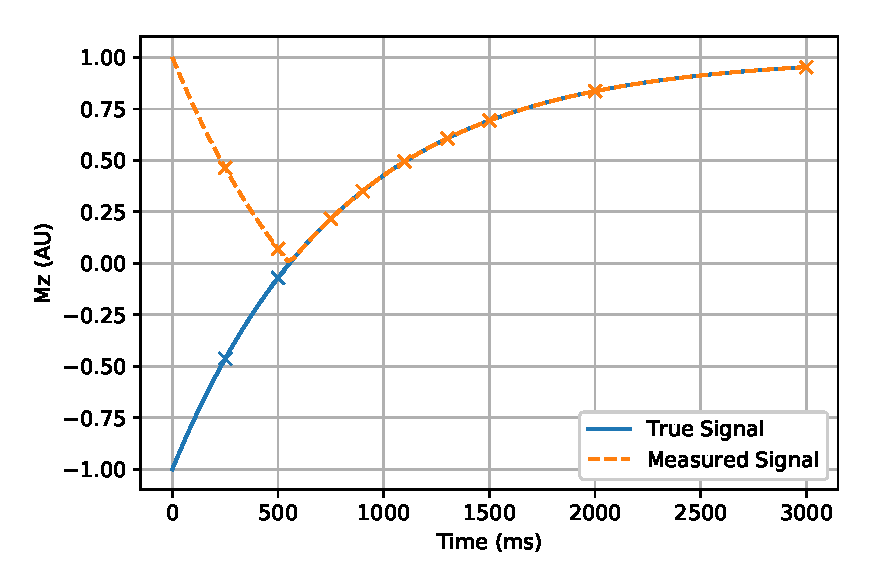
\includegraphics[width=0.5\textwidth]{neph/signal_correction.eps}
	\caption{A simulation of the true and measured magnetisation for a $T_1$ of 800 ms. The crosses represent the inversion times at which the inversion recovery is sampled.}
	\label{fig:sig_correction}	
\end{figure}

Once the data has been polarity corrected a voxel by voxel least squares trust region reflective  method is used to fit the data to Equation \eqref{eq:T1} and estimate the $T_1$ and $M_0$ of the tissue in that voxel along with an uncertainty in the fit \cite{branch_subspace_1999}. This data processing is carried out using an in-house Python package. Once the $T_1$ maps are generated, \ac{ROI} are defined for the renal medulla and renal cortex and the mean $T_1$ in these \ac{ROI} recorded.

\begin{equation}
M_z = M_0 \left(1-2\cdot e^{-TI/T_1}\right)
\label{eq:T1}
\end{equation}

\subsection{$T_2$ Mapping}
\label{subsec:neph_t2_mapping}

Compared to other quantitative renal measurements, $T_2$ mapping is still relatively unexplore in-vivo or ex-vivo with little consensus in the community about which methods are best suited to each situation \cite{dekkers_consensus-based_2019}. This lack of consensus and existing literature meant that more work was required to establish the optimum protocol for our use case. Due to this works interest to the wider community out of the context of the nephrectomy paradigm, the development and comparison of $T_2$ mapping protocols is explored in Chapter \ref{chap:t2_mapping}.

\subsection{$T_2^*$ Mapping}
\subsubsection{Acquisition}

Ex-vivo $T_2^*$ maps can be acquired at both 3T and 7T using a multi-slice \ac{FFE} sequence with scans being performed at a range of different echo times. An example of the acquisition at each echo time is shown in Figure \ref{fig:echo_raw_data}

\begin{figure}[H]
	\centering
	%\missingfigure{Individual TE scans}
	\includegraphics[width=0.8\textwidth]{Neph/Individual_TE.eps}
	\caption{Acquisitions at each of the \ac{TE} at 7T.}
	\label{fig:echo_raw_data}	
\end{figure}

The acquisition parameters at 3T are \ac{FOV} = 145 $\times$ 145 $\times$ 15 mm, voxel size = 0.6 $\times$ 0.6 $\times$ 1.5 mm$^3$, \ac{TR} = 697 ms, \ac{FA} = $38\degree$, \ac{SENSE} Factor = 2.0, Acquisition Time $\approx$ 180 sec per \ac{TE} collected. 
The acquisition parameters at 7T are \ac{FOV} = 145 $\times$ 145 $\times$ 10 mm, voxel size = 0.5 $\times$ 0.5 $\times$ 1.0 mm$^3$, \ac{FA} = $38\degree$, \ac{SENSE} Factor = 2.0, Acquisition Time $\approx$ 180 sec per \ac{TE} collected. Initially echo times were 15 ms, 20 ms, 25 ms, 30 ms, 35 ms, 40 ms and 50 ms at 3T and 10 ms, 16 ms, 22 ms, 25 ms, 28 ms and 30 ms at 7T however to reduce acquisition times, the 3T echo times were reduced to 15 ms, 20 ms, 25 ms, 40 ms and 50 ms.

\subsubsection{Analysis}
The data is fit voxel by voxel using a weighted echo time fit from the log of the exponential signal decay (Equation \eqref{eq:T2star}) to generate the $T_2^*$ maps \cite{cox_multiparametric_2017}. This data processing is carried out using an in-house Python package. The \ac{ROI} were defined using the $T_1$ weighted data if available as it has a greater cortical medullary contrast at shorter times from fixation. The mean $T_2^*$ in these \ac{ROI} is recorded.
\begin{equation}
S(t) = S_0 \cdot e^{-TE/T_2^*}
\label{eq:T2star}
\end{equation}

\subsection{Apparent Diffusion Coefficient}
\subsubsection{Acquisition}
\paragraph{Optimisation of b values}

\subsubsection{Post-Processing and Analysis}

\subsection{Diffusion Tensor Imaging}

As part of the nephrectomy protocol, Chapter \ref{chap:Neph}, we want to be able to assess the microstructure of the kidneys, one avenue to pursue for this is the use of \ac{DTI}. \ac{FA} has been shown to correlate with \ac{GFR} \cite{liu_chronic_2015} and mean tract length is an indicator of ureteropelvic junction obstruction \cite{delgado_pilot_2019} showing that tractography can be used to assess renal structure.

One of the major hurdles to overcome in developing a renal \ac{DTI} protocol for this study was correction of both \ac{EPI} readout distortions and eddy current induced distortions. This was achieved using a pipeline based around \ac{FSL}'s topup \cite{andersson_how_2003, smith_advances_2004} and eddy \cite{andersson_integrated_2016} routines. Key acquisition parameters for the sequence are 64 directions arranged over a whole spherical shell to assist with eddy current correction, this whole acquisition is then repeated with the opposite phase-encode direction to enable \ac{EPI} distortion correction. A b-value of 600 s/mm$^2$ is used. \ac{FA} maps are generated using \ac{FSL} and tractography is processed using an in-house pipeline developed using the Dipy Python library \cite{garyfallidis_dipy_2014}.

Using this pipeline, images such as those in figures \ref{fig:dti_tracts} and \ref{fig:dti_fa} could be produced. This protocol is now ready to be used on patients undergoing a nephrectomy.

\begin{figure}[H]
	\centering
	\includegraphics[width=.9\textwidth]{Other/DTI/img5c.png}
	\caption{Example tractography generated using the above protocol.}
	\label{fig:dti_tracts}
\end{figure}

\begin{figure}[H]
	\centering
	\includegraphics[width=.55\textwidth]{Other/DTI/dti_FA.png}
	\caption{An example \ac{FA} map generated using the protocol above.}
	\label{fig:dti_fa}
\end{figure}
\subsubsection{Acquisition}

\subsubsection{Post-Processing and Analysis}
\paragraph{Distortion Correction}
\paragraph{Fractional Anisotropy}
\paragraph{Tractography}

\subsection{Layer Based Analysis}

The vast majority of analysis of renal \ac{MRI} data is based around defining \ac{ROI} within the kidneys. While this method has provided excellent results, it is by no means perfect as these \ac{ROI} need to be manually defined, leading to human bias, or defined by an automated method which, as outlined in Chapter \ref{chap:ML}, can be difficult to generalise.

Taking inspiration from the analysis pipelines used by neuroimagers \cite{self_benchmarking_2019, muckli_contextual_2015, waehnert_anatomically_2014}, a method of dividing the kidneys into layers of equal thickness was developed. This method uses a three-dimensional FreeSurfer mesh on the surface of the kidney \cite{dale_cortical_1999} and levelsets to produce a map of how far each voxel is from the surface. From this map it is possible to place voxels into layers of any thickness. An example of this method being applied to both the brain and an ex-vivo kidney sample can be seen, figures \ref{fig:layers_brain} and \ref{fig:layers_kidney} respectively.

One of the main challenges in transferring this technique is coping with the reduced \ac{FOV} that comes with body imaging. Given that the method essentially asks how far is each voxel from the closes vertex on the mesh, if the mesh has a large hole in it where the slices stop covering the kidney, then the quantitative nature of this depth map is compromised.

\begin{figure}[H]
	\centering
	\begin{subfigure}[c]{0.47\textwidth}
		\centering
		\includegraphics[height=1\textwidth]{Other/Layers/mri_to_roi_to_surf_Artboard_5.eps}
		\caption{}
		\label{fig:layers_brain}
	\end{subfigure}
	\hfill
	\begin{subfigure}[c]{0.47\textwidth}
		\centering
		\includegraphics[height=1\textwidth]{Other/Layers/kidney_levelsets-02.eps}
		\caption{}
		\label{fig:layers_kidney}
	\end{subfigure}
	\caption{(\subref{fig:layers_brain}) A depth mask of the brain. Lighter areas are deeper inside the brain. (\subref{fig:layers_kidney}) A depth mask applied to a quantitative $T_1$ map.}
	\label{fig:layers_example}
\end{figure}

This levelset method was compared to two other methods of producing layers in the kidneys, a two-dimensional and a three-dimensional version of the \ac{TLCO} method \cite{piskunowicz_new_2015, milani_reduction_2017}. Each method was tested with a volume that included the entire kidney, and a cropped volume that only included the central section of the kidney, simulating the reduced \ac{FOV} that is common in body imaging. The layers generated were the applied to a $T_1$ map with the mean and standard deviation of $T_1$ in each layer being plot, Figure \ref{fig:layers_comp}.

\begin{figure}[H]
	\centering
	\begin{subfigure}[c]{0.47\textwidth}
		\centering
		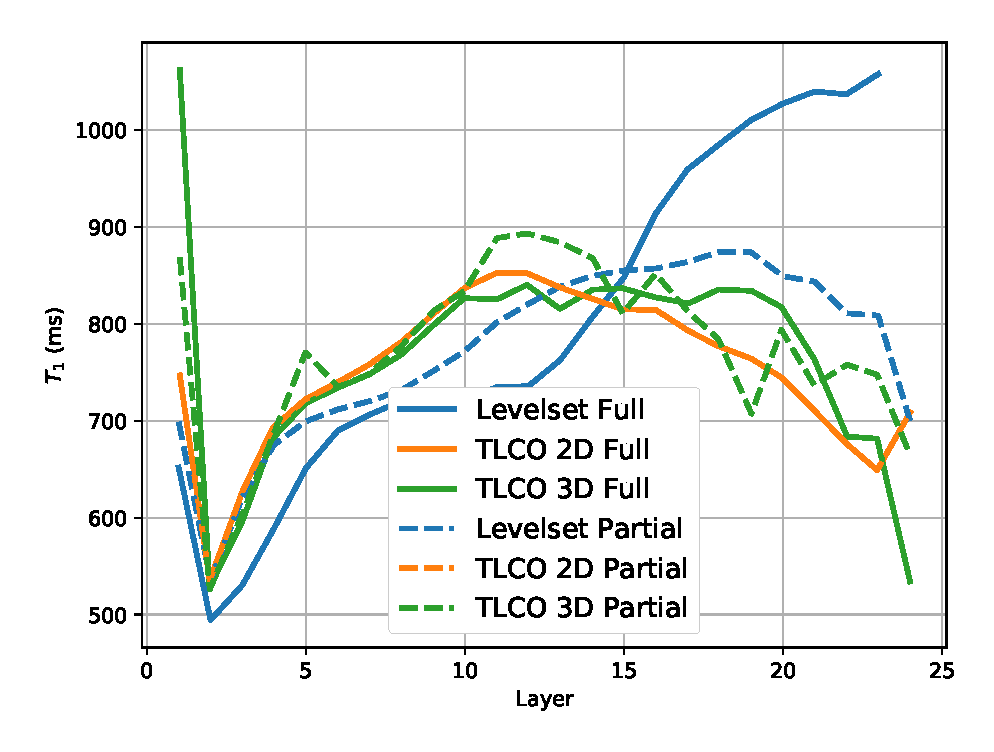
\includegraphics[width=1\textwidth]{Other/Layers/T1_crop.eps}
		\caption{}
		\label{fig:layers_t1_comp}
	\end{subfigure}
	\hfill
	\begin{subfigure}[c]{0.47\textwidth}
		\centering
		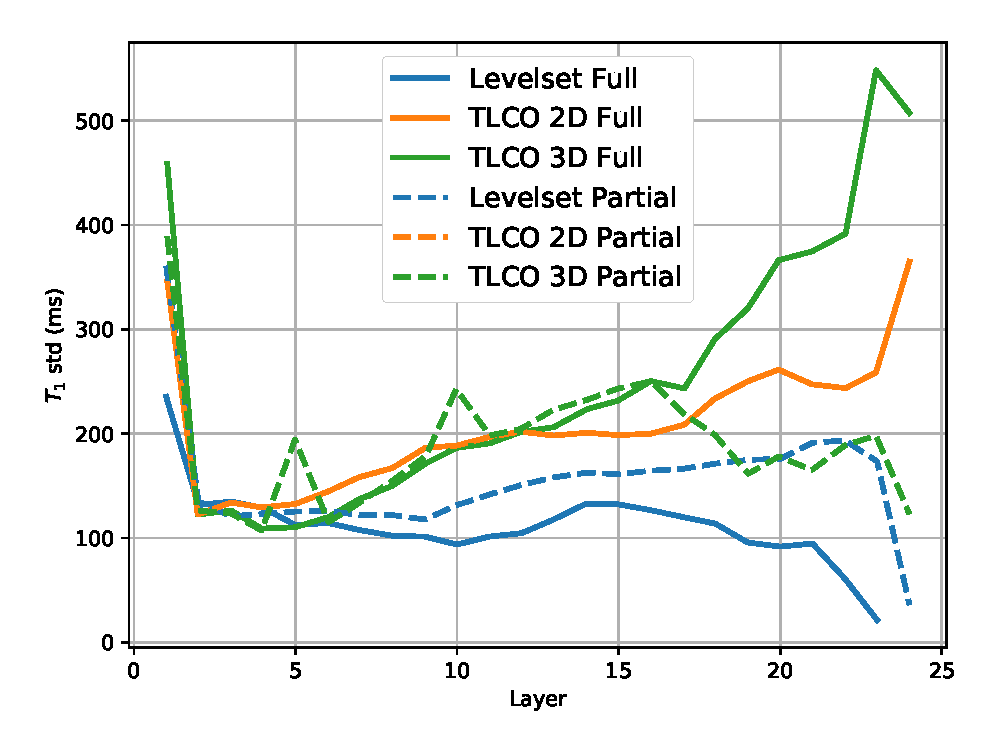
\includegraphics[width=1\textwidth]{Other/Layers/T1_std_crop.eps}
		\caption{}
		\label{fig:layers_t1_std_comp}
	\end{subfigure}
	\caption{(\subref{fig:layers_t1_comp}) The mean $T_1$ within each layers produced by each of the three methods when processing either the full volume of the kidney or only the central slices. (\subref{fig:layers_t1_std_comp}) The standard deviation of the $T_1$ within the layers produced by each method.}
	\label{fig:layers_comp}
\end{figure}

In Figure \ref{fig:layers_t1_std_comp} we can see that the layers output by the levelset method when applied to a full volume dataset produce the minimum standard deviation, this means the layers are the most anatomically sensible as a smooth transition of $T_1$ is expected with depth in the kidney and therefore the variance in each layer should be relatively small. Given this method produces the most realistic layers, other methods will be compared to it.

Neither of the \ac{TLCO} methods manage to capture the increase in $T_1$ that can be seen deeper in the kidney. They also have a much larger standard deviation per layer for deeper layers than the levelset method implying that the layers produced are a mixture of cortex and medulla. When comparing the performance of each method with only a partial volume of kidney, the levelset method produces the results that are closes to that of the full volume levelset.

Given this method can be used both in-vivo and on ex-vivo samples, they will make for an interesting additional analysis pipeline for the work in Chapter \ref{chap:Neph}.

\newpage
\section{Results and Discussion}
\label{sec:neph_results}

\subsection{Fixation and Protocol Development}
As was alluded to in Section \ref{sec:fixation}, there was significant variability in the quality of the samples collected from the slaughterhouse. This was largely due to the legislation surrounding animals slaughtered to enter the human food chain. If any part of the animal is destined for human consumption then the carcase must be thoroughly inspected before any tissue can be released. This can cause two issues. As part of the inspection, the kidneys need to be examined for parasites, this is done by making an incision in the organ, however, the quality of this incision can vary massively with some samples having a 20 mm slice cut into them while others are roughly cut in half. The second issue is caused by the variable time between slaughter and the tissue being released after inspection. For these reasons kidneys began to be procured from Veterinary Science collaborating with Prof David Gardner. The animals slaughtered there are not destined for human consumption and as such the kidneys can be placed into \ac{PBS} and subsequently \ac{NBF} far quicker and the kidneys do not need to be sliced open for inspection. The difference in the samples from these two sources can clearly be seen in Figure \ref{fig:kidney_samples}. This collaboration also enables the procurement of kidneys from a greater range of animals including different ages of pigs and therefore different degrees of fibrosis and inducing \ac{AKI} in the animals prior to scanning and histology. Veterinary Science can also carry out the histology in house, thus streamlining the protocol by avoiding transporting one kidney to Derby for histology and the other to \ac{SPMIC} for scanning.

\begin{figure}[H]
	\centering
	\begin{subfigure}[c]{0.9\textwidth}
		\centering
		\begin{subfigure}[c]{0.47\textwidth}
			\centering
			\includegraphics[width=0.9\textwidth, angle=180]{neph/meat_kidney}
			\caption{}
			\label{fig:meat_kidney}
		\end{subfigure}
		\hfill
		\begin{subfigure}[c]{0.47\textwidth}
			\centering
			\includegraphics[width=0.9\textwidth, angle=180]{neph/sb_kidney}
			\caption{}
			\label{fig:sb_kidney}
		\end{subfigure}
	\end{subfigure}
	\vskip\baselineskip
	\begin{subfigure}[c]{0.9\textwidth}
		\centering
		\begin{subfigure}[c]{0.47\textwidth}
			\centering
			\includegraphics[width=0.9\textwidth]{neph/meat_mri}
			\caption{}
			\label{fig:meat_mri}			
		\end{subfigure}
		\hfill
		\begin{subfigure}[c]{0.47\textwidth}
			\centering
			\includegraphics[width=0.9\textwidth, angle=270]{neph/sb_mri}
			\caption{}
			\label{fig:sb_mri}
		\end{subfigure}
	\end{subfigure}
	\caption{(\subref{fig:meat_kidney}) An example of a sample procured from the slaughterhouse after it has been fixed. The left hand kidney has been sliced in half; the right hand kidney has the incisions from the meat inspector clearly visible. (\subref{fig:sb_kidney}) An example of a sample procured from Veterinary Science post fixing. (\subref{fig:meat_mri}) An example of a $T_2$ weighted FFE with TE = 40 ms of a kidney procured from the slaughterhouse. (\subref{fig:sb_mri}) An example of a $T_2$ weighted FFE with TE = 40 ms of a kidney procured from Veterinary Science.} 
	\label{fig:kidney_samples}
\end{figure}

Once samples had been fixed and transferred to \ac{PBS} they could be placed into the scanner. Using the protocols outlined above it was possible to generate maps as shown in Figure \ref{fig:neph_maps}.

\begin{figure}[H]
	\centering
	\begin{subfigure}[c]{0.9\textwidth}
		\centering
		\begin{subfigure}[c]{0.47\textwidth}
			\centering
			\includegraphics[width=1\textwidth]{Neph/T1_map_3T.eps}
			\caption{}
			\label{fig:neph_t1_map_3t}
		\end{subfigure}
		\hfill
		\begin{subfigure}[c]{0.47\textwidth}
			\centering
			\includegraphics[width=1\textwidth]{Neph/T2star_map_3T.eps}
			\caption{}
			\label{fig:neph_t2star_map_3t}
		\end{subfigure}
	\end{subfigure}
	\vskip\baselineskip
	\begin{subfigure}[c]{0.9\textwidth}
		\centering
		\begin{subfigure}[c]{0.47\textwidth}
			\centering
			\includegraphics[width=1\textwidth]{Neph/T1_map_7T.eps}
			\caption{}
			\label{fig:neph_t1_map_7t}			
		\end{subfigure}
		\hfill
		\begin{subfigure}[c]{0.47\textwidth}
			\centering
			\includegraphics[width=1\textwidth]{Neph/T2star_map_7T.eps}
			\caption{}
			\label{fig:neph_t2star_map_7t}
		\end{subfigure}
	\end{subfigure}
	\caption{(\subref{fig:neph_t1_map_3t}) $T_1$ map of a kidney twenty four hours after fixation at 3T (\subref{fig:neph_t2star_map_3t}) $T_2^*$ map twenty four hours after fixation at 3T (\subref{fig:neph_t1_map_7t}) $T_1$ map twenty four hours after fixation at 7T (\subref{fig:neph_t2star_map_7t}) $T_2^*$ map twenty four hours after fixation at 7T. The sample shown in the 3T and 7T figures is different.} 
	\label{fig:neph_maps}
\end{figure}

\subsection{Monitoring Changes in MR Parameters Post Fixation}
\label{sec:longevity}
To study the effects of the fixation process upon MR measurements, a kidney was fixed as per the method in Section \ref{sec:fixation} and scanned at both field strengths of 3T and 7T. Collecting a $T_1$ and $T_2^*$ map took approximately 90 minutes per field strength. Once the maps had been generated, \ac{ROI} were defined and the mean $T_1$ and $T_2^*$ for the cortex and the medulla were calculated. The sample was monitored for ten weeks. The variation in $T_1$ and $T_2^*$ over time can be seen in Figure \ref{fig:fixation_lts}.

\begin{figure}[H]
	\centering
	\begin{subfigure}[c]{0.9\textwidth}
		\centering
		\begin{subfigure}[c]{0.47\textwidth}
			\centering
			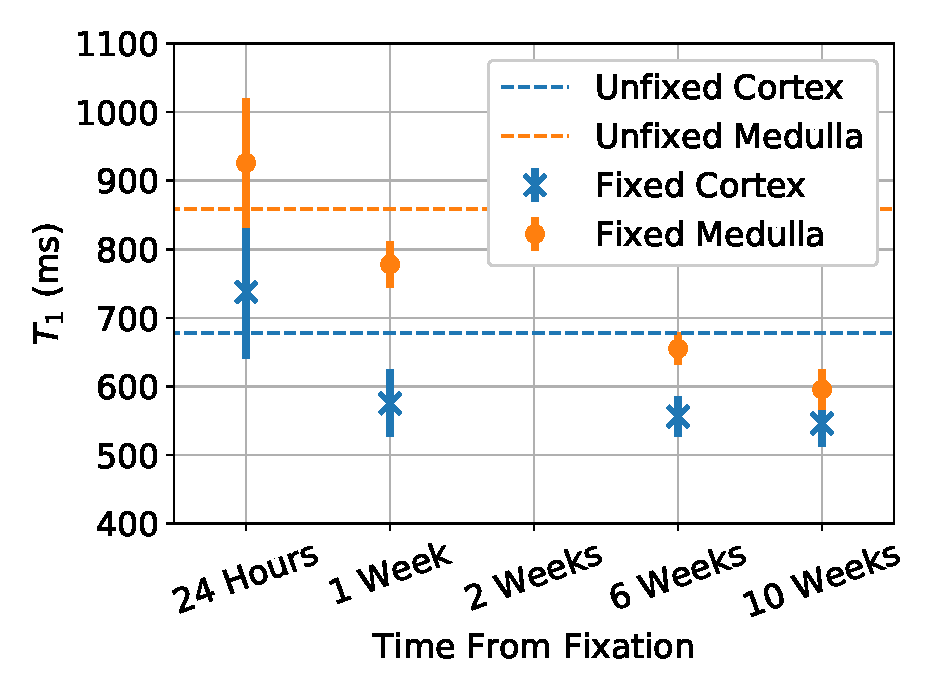
\includegraphics[width=1\textwidth]{Neph/T1_3T_crop.eps}
			\caption{}
			\label{fig:fixation_t1_3t_lts}
		\end{subfigure}
		\hfill
		\begin{subfigure}[c]{0.47\textwidth}
			\centering
			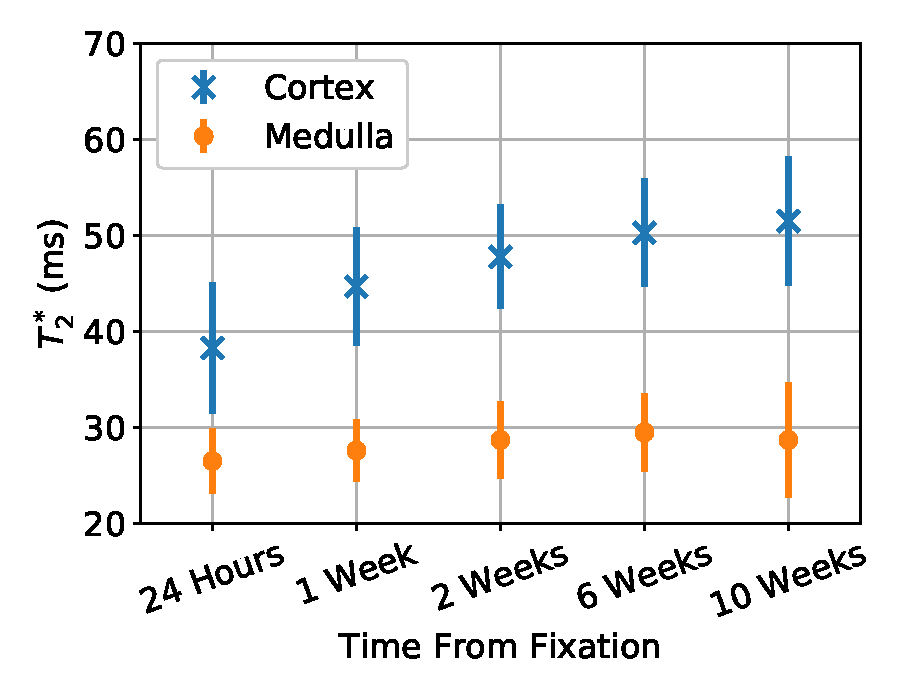
\includegraphics[width=1\textwidth]{Neph/T2star_3T_crop.eps}
			\caption{}
			\label{fig:fixation_t2star_3t_lts}
		\end{subfigure}
	\end{subfigure}
	\vskip\baselineskip
	\begin{subfigure}[c]{0.9\textwidth}
		\centering
		\begin{subfigure}[c]{0.47\textwidth}
			\centering
			\includegraphics[width=1\textwidth]{Neph/T1_7T_crop.eps}
			\caption{}
			\label{fig:fixation_t1_7t_lts}
		\end{subfigure}
		\hfill
		\begin{subfigure}[c]{0.47\textwidth}
			\centering
			\includegraphics[width=1\textwidth]{Neph/T2star_7T_crop.eps}
			\caption{}
			\label{fig:fixation_t2star_7t_lts}
		\end{subfigure}
	\end{subfigure}
	\caption{(\subref{fig:fixation_t1_3t_lts}) Variation in $T_1$ as a function of time after fixation measured at 3T (\subref{fig:fixation_t2star_3t_lts}) Variation in $T_2^*$ as a function of time after fixation measured at 3T (\subref{fig:fixation_t1_7t_lts}) Variation in $T_1$ as a function of time after fixation measured at 7T (\subref{fig:fixation_t2star_7t_lts})  Variation in $T_2^*$ as a function of time after fixation measured at 7T.}
	\label{fig:fixation_lts}
\end{figure}

Unfortunately due to technical scanner issues, we were not able to scan the sample at 7T at ten weeks and the quality of the 3T $T_1$ acquisition at two weeks was significantly inferior; as such these data points have been omitted. It can be seen that the largest changes in $T_1$ and $T_2^*$ occur between twenty four hours and one week after fixation, after that there is a general trend that the $T_1$ of the cortex and medulla converge while the $T_2^*$ of each tissue type diverges, one could argue that the $T_2^*$ of the cortex measured at 3T is plateauing. This means that, although the samples will reach a steady state, in the first few weeks after fixation, their $T_1$ and $T_2^*$ will have a dependence on time. This necessitates the need to standardise the protocol, specifically the time at which the samples are scanned. It would have been useful to know the $T_1$ and $T_2^*$ of unfixed porcine kidneys and as such, a fresh, unfixed kidney was scanned using the same protocol. Unfortunately, due to the difference in stiffness between fixed and unfixed kidneys, the same protocol did not deliver usable $T_2^*$ data as the unfixed kidney vibrated too much while floating in the \ac{PBS}. This problem could potentially be reduced by either vibration insulation between the sample and the scanner as per Dawe et al \cite{dawe_postmortem_nodate} or by embedding the sample in an agarose medium rather than allowing it to float in \ac{PBS} as per Kolk et al\cite{kolk_imaging_2014}. The $T_1$ of the unfixed kidney was seen to be between that of the fixed kidney between 24-hours and one week.

To investigate this time dependence over a shorter time scale, a pair of kidneys were acquired and fixed as before. It will be possible to scan most human samples within 24 hours of fixation, as such it is desirable to see how much $T_1$, $T_2^*$ and histology change over this period. Scanning was only carried out at 3T as more frequent measurements were preferable to measurements at different field strengths. For this reason the number of inversion times and echo times used to generate the $T_1$ and $T_2^*$ maps was reduced to \ac{TI} = 400 ms, 500 ms, 750 ms, 900 ms, 1100 ms, 2600 ms and \ac{TE} = 15 ms, 20 ms, 25 ms, 40 ms, 50 ms respectively. The choice of these inversion/echo times was arrived at empirically by carrying out the analysis pipeline on a single slice of data using each combination of six and five of the previously used \ac{TI}s and \ac{TE}s respectively. The results from each combination of \ac{TI}/\ac{TE} were compared to those generated when using the full complement of inversion/echo times and the combination delivering the minimum difference chosen. This reduction in the number of inversion times resulted in a mean error per voxel in the kidney of 20.9 $\pm$ 12.3 ms if the full complement of inversion times was taken as the ground truth, the reduction in echo times resulted in a mean error of 0.3 $\pm$ 1.2 ms.

Scanning sessions started at 1.5 hours, 2.5 hours, 4 hours, 5.5 hours, 19 hours and 22 hours after the sample was removed from the \ac{NBF}. Due to the potential for the properties to change relatively quickly, especially $T_1$, it was decided to randomise the order in which the inversion/echo times were collected, this way any change in $T_1$/$T_2^*$ over the 30/20 minute acquisition period would manifest itself as non-systematic noise and thus will increase the uncertainty in the fit rather than affecting the predicted value. At the start of each scanning session, a biopsy was performed on the kidney not being scanned. Masson's trichrome and \ac{H and E} staining was performed on these samples.

\begin{figure}[H]
	\centering
	\begin{subfigure}[c]{0.47\textwidth}
		\centering
%		\missingfigure{T1 vs Times (STS)}
		\includegraphics[width=1\textwidth]{Neph/STS_T1_line.eps}
		\caption{}
		\label{fig:fixation_t1_3t_sts}
	\end{subfigure}
	\hfill
	\begin{subfigure}[c]{0.47\textwidth}
		\centering
%		\missingfigure{T2* vs Times (STS)}
		\includegraphics[width=1\textwidth]{Neph/STS_T2star_line.eps}
		\caption{}
		\label{fig:fixation_t2star_3t_sts}
	\end{subfigure}
	\caption{(\subref{fig:fixation_t1_3t_sts}) Variation in $T_1$ as a function of time after fixation measured at 3T (\subref{fig:fixation_t2star_3t_sts}) Variation in $T_2^*$ as a function of time after fixation measured at 3T.}
	\label{fig:fixation_sts}
\end{figure}

No significant change in $T_1$ or $T_2^*$ was observed over the period the sample was monitored. This is promising as it means that when this protocol is applied to human samples, there will be a relatively large time window in which the ex-vivo scan can be carried out, making the experimental procedure simpler. The corresponding histology results showed no change in the cortex over this period however there was a noticeable inflammatory response in the medulla.

It was noted that the sample used for this experiment was not of especially high quality, the kidney has two slices in it, one that almost bifurcated the sample along the coronal plane, another cut down one half of the sample along the sagittal plane, visible in Figure \ref{fig:fixation_t1map_3t_sts}. These cuts meant that air became trapped within the sample causing it to float in the \ac{PBS}. If not corrected this would cause large susceptibility artefacts where the sample came into contact with the air at the top of the \ac{PBS}; to remedy this the sample was entirely bifurcated. Despite the best efforts of investigators, air bubbles remained in the sagittal slice, causing the aforementioned artefacts, especially visible in Figure \ref{fig:fixation_t2starmap_3t_sts}. Given these concerns over sample quality, it was decided to scan the sample again one week after fixation, to match the time period in the previous experiment (Figure \ref{fig:fixation_lts}).

\begin{figure}[H]
	\centering
	\begin{subfigure}[c]{0.47\textwidth}
		\centering
		\includegraphics[width=1\textwidth]{Neph/T1_map_STS.eps}
		\caption{}
		\label{fig:fixation_t1map_3t_sts}
	\end{subfigure}
	\hfill
	\begin{subfigure}[c]{0.47\textwidth}
		\centering
		\includegraphics[width=1\textwidth]{Neph/T2star_map_STS.eps}
		\caption{}
		\label{fig:fixation_t2starmap_3t_sts}
	\end{subfigure}
	\caption{(\subref{fig:fixation_t1map_3t_sts}) An example of the $T_1$ map collected from the short time scale kidney (\subref{fig:fixation_t2starmap_3t_sts}) An example of the $T_2^*$ map collected from the short time scale kidney.}
	\label{fig:neph_maps_sts}
\end{figure}

It was expected that upon repeating the measurements one week later, the $T_1$ of both cortex and medulla would decrease and the $T_2^*$ of the cortex would increase. This was not the case, there was a slight decrease in the $T_1$ of the medulla but otherwise, no change was observed, Figure \ref{fig:fixation_mts}. This lead us to conclude that the large cuts in the sample had lead to a different level of fixation. Subsequent to this, samples were to be procured from Veterinary Science as they are more consistent and therefore more akin to the human samples that will be used.

\begin{figure}[H]
	\centering
	\begin{subfigure}[c]{0.47\textwidth}
		\centering
%		\missingfigure{T1 vs Times (MTS)}
		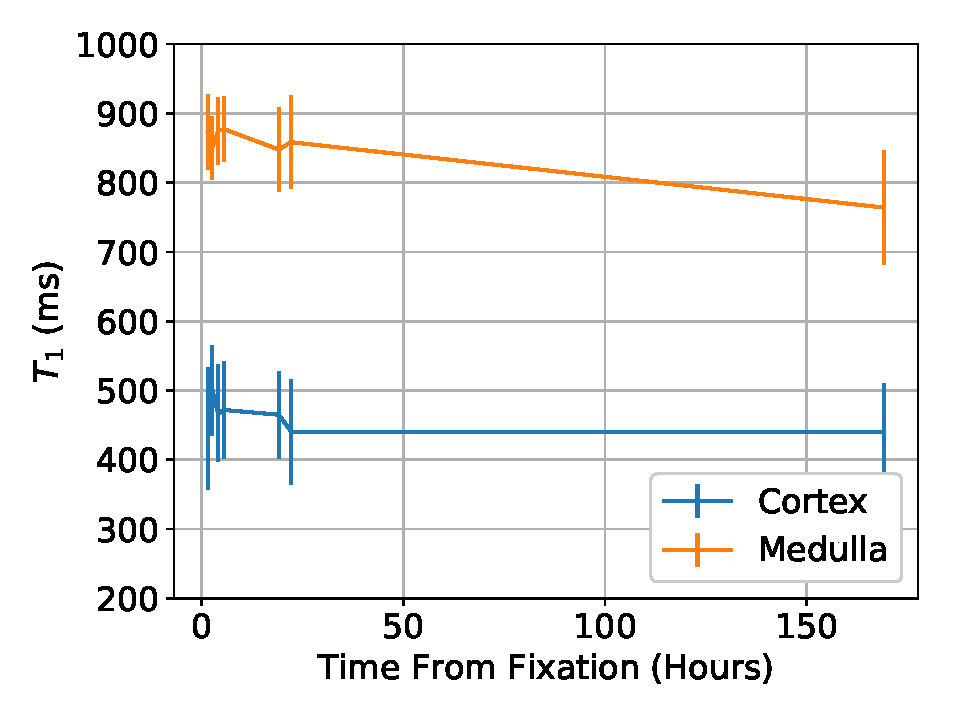
\includegraphics[width=1\textwidth]{Neph/MTS_T1_line.eps}
		\caption{}
		\label{fig:fixation_t1_3t_mts}
	\end{subfigure}
	\hfill
	\begin{subfigure}[c]{0.47\textwidth}
		\centering
%		\missingfigure{T2* vs Times (MTS)}
		\includegraphics[width=1\textwidth]{Neph/MTS_T2star_line.eps}
		\caption{}
		\label{fig:fixation_t2star_3t_mts}
	\end{subfigure}
	\caption{(\subref{fig:fixation_t1_3t_mts}) Variation in $T_1$ as a function of time after fixation measured at 3T (\subref{fig:fixation_t2star_3t_mts}) Variation in $T_2^*$ as a function of time after fixation measured at 3T.}
	\label{fig:fixation_mts}
\end{figure}

\subsection{Comparing MR and Histological Measures in Aged Kidneys}

To verify the correlation of MR measurements with histology, kidneys were collected from a 0.5 year old and 2.5 year old pig. These different ages were expected to have differing levels of renal inflammation and fibrosis. Figure \ref{fig:aged_map} shows example \ac{MRI} data collected from these samples, Figure \ref{fig:aged_bar} shows the quantitative differences in $T_1$ and $T_2^*$ between the two samples.

\begin{figure}[H]
	\centering
	\begin{subfigure}[c]{0.47\textwidth}
		\centering
		\includegraphics[width=1\textwidth]{Neph/aged_kidneys/Young_T1.eps}
		\caption{}
		\label{fig:neph_aged_t1_map}
	\end{subfigure}
	\hfill
	\begin{subfigure}[c]{0.47\textwidth}
		\centering
		\includegraphics[width=1\textwidth]{Neph/aged_kidneys/Old_T1.eps}
		\caption{}
		\label{fig:neph_aged_t2star_map}
	\end{subfigure}
	\caption{(\subref{fig:neph_aged_t1_map}) $T_1$ map of a 0.5 year old pig kidney. (\subref{fig:neph_aged_t2star_map}) $T_1$ map of a 2.5 year old pg kidney.}
	\label{fig:aged_map}
\end{figure}

\begin{figure}[H]
	\centering
	\begin{subfigure}[c]{0.47\textwidth}
		\centering
		\includegraphics[width=1\textwidth]{Neph/aged_kidneys/T1_bar.eps}
		\caption{}
		\label{fig:neph_aged_t1_bar}
	\end{subfigure}
	\hfill
	\begin{subfigure}[c]{0.47\textwidth}
		\centering
		\includegraphics[width=1\textwidth]{Neph/aged_kidneys/T2star_bar.eps}
		\caption{}
		\label{fig:neph_aged_t2star_bar}
	\end{subfigure}
	\caption{(\subref{fig:neph_aged_t1_bar}) The $T_1$ of the renal cortex and medulla of the two samples. (\subref{fig:neph_aged_t2star_bar}) The $T_2^*$ of the renal cortex and medulla of the two samples.}
	\label{fig:aged_bar}
\end{figure}

No significant change is observed in the $T_1$ or $T_2^*$ of cortex the two kidneys. There is however a decrease in $T_1$ seen in the medulla of the older kidney. Cortical samples were removed from the same animals for histological analysis. These samples were stained using \ac{H and E} and Masson's trichrome to enable the evaluation of levels of fibrosis, these micrographs are shown in Figure \ref{fig:aged_histo}. 

\begin{figure}[H]
	\centering
	\begin{subfigure}[c]{0.9\textwidth}
		\centering
		\begin{subfigure}[c]{0.47\textwidth}
			\centering
			\includegraphics[width=1\textwidth]{Neph/aged_kidneys/Figure_5_V3_Young_H_and_E.png}
			\caption{}
			\label{fig:neph_young_h_and_e}
		\end{subfigure}
		\hfill
		\begin{subfigure}[c]{0.47\textwidth}
			\centering
			\includegraphics[width=1\textwidth]{Neph/aged_kidneys/Figure_5_V3_Old_H_and_E.png}
			\caption{}
			\label{fig:neph_old_h_and_e}
		\end{subfigure}
	\end{subfigure}
	\vskip\baselineskip
	\begin{subfigure}[c]{0.9\textwidth}
		\centering
		\begin{subfigure}[c]{0.47\textwidth}
			\centering
			\includegraphics[width=1\textwidth]{Neph/aged_kidneys/Figure_5_V3_Young_Trichrome.png}
			\caption{}
			\label{fig:neph_young_trichrome}			
		\end{subfigure}
		\hfill
		\begin{subfigure}[c]{0.47\textwidth}
			\centering
			\includegraphics[width=1\textwidth]{Neph/aged_kidneys/Figure_5_V3_Old_Trichrome.png}
			\caption{}
			\label{fig:neph_old_trichrome}
		\end{subfigure}
	\end{subfigure}
	\caption{(\subref{fig:neph_young_h_and_e}) A sample of renal cortex from a 0.5 year old pig stained with \ac{H and E}. (\subref{fig:neph_old_h_and_e}) A sample of renal cortex from a 2.5 year old pig stained with \ac{H and E}. (\subref{fig:neph_young_trichrome}) A sample of renal cortex from a 0.5 year old pig stained with Masson's trichrome. (\subref{fig:neph_old_trichrome}) A sample of renal cortex from a 2.5 year old pig stained with Masson's trichrome.} 
	\label{fig:aged_histo}
\end{figure}

No significant difference is seen between the histology of these cortical samples. This means that \ac{MRI} and histology are in agreement. Unfortunately no samples were taken from the renal medulla, the area which showed a change in MR measurements. In future samples with a larger difference in age should be used as these will have a greater difference in fibrosis and samples should be taken from the medulla for histological analysis.

\section{Conclusions and Future Work}

This chapter shows progress towards correlating renal \ac{MRI} measurements with histology. We are able to acquire high resolution $T_1$, $T_2$, $T_2^*$ maps. We have also developed protocols to carry out simultaneous biopsy for histology and \ac{MRI} acquisition. These protocols have shown that the $T_1$ and $T_2^*$ of the kidneys are not constant after fixation however there is a window of 24-hours after fixation in which scanning is optimum. We have also shown that these measures agree with histology. Below are listed some of the directions in which future work could explore.

\subsection{Protocol Validation on a Single Sample}

As each protocol, including those in Section \ref{sec:dti}, has been developed separately, they have not been carried out on the same sample, as the intention is to use all the protocols outlined in Section \ref{sec:neph_methods} on each nephrectomy sample, it would be useful to collect all protocols on a single sample. This could be coupled with a repeat investigation into the effects of ageing by collecting data from kidneys with a larger difference in ages.

\subsection{Ex-Vivo Sample Coil}
Sengupta demonstrated the benefits of using custom made ex-vivo sample coils in human scanners \cite{sengupta_high_2017}. Currently scanning uses the standard head coils however this results in a relatively large distance between sample and coils as seen in Figure \ref{fig:head_coil}. There would certainly be improvements in data quality if a coil specifically designed for small sample imaging at 7T were fabricated.
\begin{figure}[H]
	\centering
	\includegraphics[width=0.5\textwidth]{Neph/head_coil.jpg}
	\caption{A sample sat within the 32 channel 3T head coil. A bespoke ex-vivo sample coil would have less space between the coil and the sample.}
	\label{fig:head_coil}	
\end{figure}

\subsection{Human Organs}
All work thus far has been using porcine kidneys. While these provide an excellent model for protocol development due to their similarities to human kidneys, the utility of this investigation will be enhanced massively when human organs are studied. To this end, once the development work has been completed and protocols finalised, samples will begin to be procured from subjects undergoing a nephrectomy as part of their standard clinical care.

Another source of human organs are those rejected for transplant. Due to the relatively small time window in which a transplant centre has between an organ donation being made and the organ losing its transplant viability, a large number of human kidneys are unable to be successfully donated. While not suitable for transplant any more, these organs would still be useful in providing ex-vivo \ac{MRI} data and histology in the healthy population. There are pre-existing agreements enabling failed transplant tissue to be used in scientific research, as such, this would be an interesting avenue to explore.

\section{Acknowledgements}

We are grateful for access to the University of Nottingham's Augusta high performance computing service.

\newpage
\section{References}
\defbibheading{bibliography}[\refname]{}
\printbibliography

\newpage

\chapter{Automated Segmentation of Kidneys using Machine Learning}
\label{chap:ML}

\begin{abstract}
	\ac{TKV} is an important measure in renal disease detection and monitoring. Here a fully automated method to segment the kidneys from \ttwo-weighted \ac{MRI} to calculate \ac{TKV} of \ac{HC} and \ac{CKD} patients is developed.
	
	This automated method uses machine learning, specifically a 2D \ac{CNN}, to accurately segment the left and right kidneys from \ttwo-weighted \ac{MRI} data. The dataset consisted of 30 \ac{HC} subjects and 30 \ac{CKD} patients. The model was trained on 50 manually defined \ac{HC} and \ac{CKD} kidney segmentations. It was subsequently evaluated on 50 test data sets, comprising data from five \ac{HC}s and five \ac{CKD} patients each scanned five times in a scan session to enable comparison of the precision of the \ac{CNN} and manual segmentation of kidneys.
	
	The unseen test data processed by the 2D \ac{CNN} had a mean Dice score of 0.93 $\pm$ 0.01. The difference between manual and automatically computed \ac{TKV} was 1.2 $\pm$ 16.2 m$\ell$ with a mean surface distance of 0.65 $\pm$ 0.21 mm. The variance in \ac{TKV} measurements from repeat acquisitions on the same subject was significantly lower using the automated method compared to manual segmentation of the kidneys.
	
	The 2D \ac{CNN} method provides fully automated segmentation of the left and right kidney and calculation of \ac{TKV} in under ten seconds on a standard office computer, allowing high data throughput and is a freely available executable.
	
	This work was presented as an aural presentation at the \ac{ISMRM} 28th Annual Meeting (2020) \cite{daniel_automated_2020}.
\end{abstract}
\newpage
\acresetall
\section{Introduction}

Segmentation of the kidneys from \ac{MRI} is a time consuming aspect of many renal \ac{MRI} studies \cite{cox_multiparametric_2017, cohen_mri_2009, van_den_dool_functional_2005}. \ac{TKV} gives insight into renal function and is therefore used as a measured parameter for a variety of renal pathologies. The use of \ac{TKV} is an active area of ongoing research for \ac{ADPKD}, which is characterised by an increase in \ac{TKV} due to cyst formation. Disease progression can be monitored by recording \ac{TKV}, with higher rates of \ac{TKV} increase being associated with a more rapid decrease in renal function \cite{chapman_kidney_2012, tangri_total_2017, grantham_volume_2006}. Measurements of \ac{TKV} in \ac{CKD} subjects have shown a significant correlation with glomerular filtration rate \cite{buchanan_quantitative_2019}, the primary measure of \ac{CKD} severity \cite{stevens_assessing_2006}, with more generally a decrease in \ac{TKV} associated with a decrease in renal function \cite{gong_relationship_2012}. When studying pathologies which commonly lead to a change in kidney function, total kidney perfusion is often measured, this metric relies on an accurate measurement of renal blood flow and kidney volume of each kidney, and allows investigators to ascertain if the blood flow is preserved as the organ changes in size or if tissue perfusion is impaired. In addition to \ac{TKV} measurements, renal segmentation is an important first step for many other processing pipelines, be that for automated cortical-medullary segmentations or to carry out multiparametric mapping within only the kidney to reduce computation times. 

The gold standards of kidney segmentation are manual \ac{ROI} boundary tracing \cite{di_leo_measurement_2011} or stereology \cite{bae_volumetric_2000} by experienced and skilled experts, with blood vessels in the kidney and the hilum excluded. These manual processes are highly time consuming (taking approximately 15 – 30 minutes per subject \cite{zollner_assessment_2012, sharma_kidney_2017, simms_rapid_2019} and can be biased by investigator judgement due to the similar signal intensities between the kidneys and surrounding organs, anatomical differences between subjects, cysts and image artefacts. Consequently, the resulting kidney \ac{ROI}s produced are subject to intra- and inter-expert variability as a result of the varying expertise levels; experts may segment a specific image differently when performed more than once, or different experts may segment the same image differently. These factors mean that the development of a faster and ideally fully automated method of renal segmentation is highly desirable. However the same factors that make manual segmentation difficult can also limit fully automated methods, for example the signal intensity of the kidneys closely matches that of other abdominal structures such as the spleen.
\newpage
A number of automated methods have been proposed with varied success \cite{zollner_assessment_2012}. Some simply assume the kidney is an ellipse and calculate the volume from measurements of the pole-to-pole distance \cite{cheong_normal_2007, spithoven_estimation_2015} or include a correction factor to reduce overestimations \cite{seuss_development_2017}. Unfortunately these techniques produce a large confidence interval and still require human intervention to define the pole-to-pole length, a process that can produce inconsistencies between readers and takes a reasonable amount of time ($\approx$5 min) \cite{magistroni_review_2018}. Other semi-automated methods use classical image processing techniques such as thresholding \cite{coulam_measurement_2002}, water-shedding \cite{karstoft_different_2007}, level sets \cite{simms_rapid_2019, gloger_prior_2012}, and spatial prior probability mapping \cite{kim_automated_2016}. These methods can either be inaccurate, over-segmenting the kidneys, or include a number of parameters that need to be manually adjusted and are computationally intensive. Further, the fact that each technique is highly optimised for a specific dataset means that it needs to be re-written to be applied to different pathology, another time consuming and highly skilled process.

Machine learning methods have the potential to automatically detect different patterns from data given to a model which has been trained. Deep learning is a class of machine learning algorithms that can model high-level information in an image using several processing layers of transformations. This uses an architecture of multi-level linear and non-linear operations, described by layers, to learn complex functions that can represent high-level detail to map the input data to the output segmentations directly. As more data becomes available the algorithm can become more accurate and generalised, without a need to rewrite the underlying methods, thus making it a good choice for long term development. 

In recent years, deep learning-based methods have been applied to the segmentation of medical images, especially successful has been the U-Net \cite{ronneberger_u-net_2015}. This modified fully \ac{CNN} architecture uses a number of convolution, pooling and up-sampling layers to detect features in the input data at multiple resolutions. The convolution layers convolve a learnable kernel with the input data to generate spatial feature maps that are passed to subsequent layers in the network. By adjusting the kernels, the resulting feature maps can be optimised to detect the location of the kidneys. Pooling layers are used to down-sample the data and allow some convolution kernels to become tuned to approximate features, this also reduces the tendency of the network to overfit the training data. When the data has been fully down-sampled, up-sampling layers are used to increase the resolution of the feature maps back to that of the original data while more convolution layers also learn the precise location of the kidneys. Parameters are adjusted by comparing the output from the network to a known ground truth. \ac{CNN} methods have been applied to segmentation in other areas of medical imaging \cite{lu_automatic_2017, sharma_automatic_2017, wachinger_deepnat_2018, fu_novel_2018}, for example to prostate segmentation of \ac{MRI} images \cite{hassanzadeh_convolutional_2019}, liver segmentation of x-ray \ac{CT} images \cite{li_h-denseunet_2018} and segmentation of polycystic kidneys \cite{kline_performance_2017, van_gastel_automatic_2019, shin_expert-level_2020}. However, to date, these methods have not been successfully applied to \ac{CKD} and healthy kidney segmentation from MR images. 

Here a single 2D U-Net model \ac{CNN} is used for the segmentation of the kidneys in both \ac{HC} participants and \ac{CKD} patients using \ttwo-weighted MR images. Automatically generated kidney masks are compared with manual masks defined by experts and assessed for similarity using multiple voxel and surface based metrics and total segmented volume. A subset of subjects were scanned multiple times to assess the repeatability of the segmentations.

\newpage

\section{Neural Networks for Image Segmentation}

\subsection{Artificial Neural Networks}
\acp{ANN} aim to solve computational problems using a similar methodology to their biological namesake. Input data is passed through a series of connected nodes or neurons, each of which can have multiple input and output connections from and to other neurons mimicking synapses. At each neuron, a weighted sum of the input values is calculated before being passed onto the next hidden layer of neurons. The final layer of neurons is connected to the output layer which will give an estimation of the desired property, be that a number e.g. probability someone will like a television program, an image e.g. the probability that a pixel in an image is a road sign, or a sample in a time series e.g. audio in voice synthesis. More concisely, an \ac{ANN} can be used to map a non-linear set of input data to an output dimension.

A very basic example could use the mass and colour of an animal to guess if it is a dog or a cat, Figure \ref{fig:ml_theory_init}. The connections between neurons are initialised with random weights. 

\begin{figure}[H]
	\centering
	\includegraphics[width=0.8\textwidth]{ML/theory/ANN_init.eps}
	\caption{The \ac{ANN} initialised with random numbers trying to predict the species of a small ginger cat.}
	\label{fig:ml_theory_init}	
\end{figure}

At each neuron, a weighted sum of its inputs is taken, then an activation function applied, here a \ac{ReLU}, Figure \ref{fig:ml_theory_activation_relu}, for the hidden neurons and sigmoid, \ref{fig:ml_theory_activation_sigmoid}, for the output neurons. These activation functions allow the network to act non-linearly and are modelling the action potential of biological neurons. The \ac{ReLU} function represents a higher rate of firing for signals above zero; as it is impossible for a biological neuron to reduce its firing rate below zero, the \ac{ReLU} outputs zero when the input signal is negative. The sigmoid function maps all values between zero and one, and therefore ensures the network outputs a probability at the output nodes.

\begin{figure}[H]
	\centering
	\begin{subfigure}[c]{0.47\textwidth}
		\centering
		\includegraphics[width=1\textwidth]{ML/theory/relu.pdf}
		\caption{$\sigma (x) = max(0, x)$}
		\label{fig:ml_theory_activation_relu}
	\end{subfigure}
	\hfill
	\begin{subfigure}[c]{0.47\textwidth}
		\centering
		\includegraphics[width=1\textwidth]{ML/theory/sigmoid.pdf}
		\caption{$\sigma(x) = \frac{1}{1 + e^{-x}}$}
		\label{fig:ml_theory_activation_sigmoid}
	\end{subfigure}
	\caption{Activation functions.}
	\label{fig:ml_theory_activation}
\end{figure}

As the weights were randomly initialised, the network has incorrectly predicted that the animal is a dog. By comparing the result output from the network to the known ground truth, the weights of the network can be adjusted in a process known as back propagation, Figure \ref{fig:ml_theory_adjusted}. Hyper-parameters such as learning rate and momentum control how much each weight is adjusted in response to the input data and subsequent result.

\begin{figure}[H]
	\centering
	\includegraphics[width=0.8\textwidth]{ML/theory/ANN_back_prop.eps}
	\caption{The weightings of each connection are adjusted so the output layer produces results closer to the ground truth.}
	\label{fig:ml_theory_adjusted}	
\end{figure}

When another animal is input to the network, here a smaller, darker coloured cat, the network now correctly predicts that it is a cat, \ref{fig:ml_theory_new_data}. By repeating this procedure many times, comparing the result to ground truths and adjusting the weights, a process known as training, the network becomes more and more accurate. Once trained, the network can be used to infer the species of animals with no ground truth data.

\begin{figure}[H]
	\centering
	\includegraphics[width=0.8\textwidth]{ML/theory/ANN_new_data.eps}
	\caption{New data is presented to the network in the form of a smaller, darker coloured cat and the process of adjusting weights is repeated until more accurate results are produced.}
	\label{fig:ml_theory_new_data}	
\end{figure}

The above example is highly simplified, real \ac{ANN}s will have many more input nodes and hidden layers. In the case of imaging data, the input layer will simply be a node for each pixel in the image.

\subsection{Convolutional Neural Networks}

It was found that \ac{ANN} segmentation performance was increased if additional features were input to the network. These features could be colour rather than greyscale date, different \ac{MRI} contrasts e.g. fat/water images or artificially generated features. In Figure \ref{fig:ml_theory_features} a selection of artificially generated features are presented, some of these highlight the kidneys from the surrounding tissue e.g. the intensity range adjustment, \ref{fig:ml_theory_features_levels}, and edge detector, \ref{fig:ml_theory_features_edges} while others are better at providing contrast between the cyst in the right kidney and the renal tissue e.g. the intensity inversion, \ref{fig:ml_theory_features_invert} and sharpening filter, \ref{fig:ml_theory_features_sharpern}.

\begin{figure}[H]
	\centering
	\begin{subfigure}[c]{0.30\textwidth}
		\centering
		\includegraphics[width=1\textwidth]{ML/Theory/Features/raw.png}
		\caption{}
		\label{fig:ml_theory_features_raw}
	\end{subfigure}
	\hfill
	\begin{subfigure}[c]{0.30\textwidth}
		\centering
		\includegraphics[width=1\textwidth]{ML/Theory/Features/levels.png}
		\caption{}
		\label{fig:ml_theory_features_levels}
	\end{subfigure}
	\hfill
	\begin{subfigure}[c]{0.30\textwidth}
		\centering
		\includegraphics[width=1\textwidth]{ML/Theory/Features/invert.png}
		\caption{}
		\label{fig:ml_theory_features_invert}
	\end{subfigure}
	\vskip\baselineskip
	\begin{subfigure}[c]{0.30\textwidth}
		\centering
		\includegraphics[width=1\textwidth]{ML/Theory/Features/blur.png}
		\caption{}
		\label{fig:ml_theory_features_blur}
	\end{subfigure}
	\hfill
	\begin{subfigure}[c]{0.30\textwidth}
		\centering
		\includegraphics[width=1\textwidth]{ML/Theory/Features/sharpern.png}
		\caption{}
		\label{fig:ml_theory_features_sharpern}
	\end{subfigure}
	\hfill
	\begin{subfigure}[c]{0.30\textwidth}
		\centering
		\includegraphics[width=1\textwidth]{ML/Theory/Features/edges.png}
		\caption{}
		\label{fig:ml_theory_features_edges}
	\end{subfigure}
	\caption{An example of the features that can be generated from a raw image (\subref{fig:ml_theory_features_raw}). Implemented here are intensity range adjustments (\subref{fig:ml_theory_features_levels}), intensity inversion (\subref{fig:ml_theory_features_invert}), Gaussian blur (\subref{fig:ml_theory_features_blur}), sharpening (\subref{fig:ml_theory_features_sharpern}) and edge detection (\subref{fig:ml_theory_features_edges}).}
	\label{fig:ml_theory_features}
\end{figure}

Many of these artificially generated features can be implemented as convolutional operations, these involve convolving a numerical kernel with every pixel in the image. By adjusting the values of each cell in the kernel, different features or filters can be produced. The control of these kernels can be handed over to similar optimisation processes to those used to adjust the weights of the connections between neurons. Over the training period, this enables the network to learn what features are useful for the task at hand and which as less useful rather than the network being given features that the programmer thinks will be helpful. Shallow layers of the network usually resemble features similar to those in \ref{fig:ml_theory_features} while deeper layers represent more complex and specific objects such as, using the cat and dog example above, pointy noses to distinguish dogs and triangular ears to distinguish cats. This architecture is known as a \acl{CNN} \cite{fukushima_neocognitron_1988,lecun_gradient-based_1998}. 

To aid with feature extraction, the raw image is often downsampled by max-pooling layers, this enables different kernels to act on different scales of the image can help keep the network generalisable and avoid overfitting. The U-Net architecture \cite{ronneberger_u-net_2015} combines an arm with downsampling and feature extraction with an upsampling arm that returns the image to its initial dimensions making it especially useful for segmentations tasks.

\newpage
\section{Methods}
The study was approved by the University of Nottingham Medical School Research Ethics Committee (H14082014 and E14032013), and East Midlands Research Ethics committee REC reference: 17/LO/2036 and 15/EM/0274.

\subsection{MRI Data Acquisition}
\label{sec:ml_methods_acquisition}

All kidney \ac{MRI} scans were acquired on a 3T Philips Ingenia system (Philips Medical Systems, Best, The Netherlands) using a 2D \ttwo-weighted \ac{HASTE} sequence optimised to achieve the maximum contrast between the kidneys and surrounding tissue (\ac{TE} = 60 ms, \ac{TR} = 1300 – 1800 ms, \ac{SENSE} factor = 2.5, refocus angle 120$\degree$, bandwidth, 792 Hz, \ac{FOV} = 350 x 350 mm$^2$, voxel size = 1.5 x 1.5 x 5 mm$^3$ and a slice gap of 0.5 mm with approximately 13 coronal slices, enough to image the entire kidney \cite{petzold_building_2014, will_automated_2014}, in a single 17 - 23 s breath hold.

The dataset consisted of 60 subjects, 30 \ac{HC} (10 female, 20 male) with a mean age of 26 $\pm$ 11 (19–77) years and 30 \ac{CKD} patients (6 female, 24 male) with a mean age of 59 $\pm$ 14 (19–80) years and mean \ac{CKD} Stage 3.5 $\pm$ 1.2 (1-5). Ten of the subjects (5 \ac{HC}s and 5 \ac{CKD} patients) were scanned five times in the same scan session for use as test data. In each test data scan session, subjects were repositioned between each acquisition (removed from the scanner, asked to sit up and move on the bed), additionally the scanner operator attempted to vary the acquisition geometry between each scan while still acquiring full kidney coverage. These repeated test datasets allow the consistency of the networks ability to measure \ac{TKV} to be assessed. 

In total, 649 2D image slices from the 50 subjects in the training data and 650 2D image slices from the 10 subjects in the test data, were collected. A summary of the data collected is provided in Table \ref{tab:ml_datasets} and Figure \ref{fig:ml_true_tkv_hist}.

\subsection{Manual Segmentation}
The manual binary mask of the kidneys of each subject were generated by one of three observers (A, B and C who had been trained on kidney segmentation and had an average of 2 years of experience), with each observer segmenting data from both the training and testing datasets. Kidney boundaries were manually traced using freely available software (MRIcron \cite{rorden_neurolabuscmricron_2021}) and any area of non-renal parenchyma, such as the renal hilum and cysts, were excluded from the manual definition. Binary masks of the kidney were generated, and the volume of each kidney was computed from the product of the number of voxels in each kidney mask and the voxel volume. Separate kidney volume for the left and right kidneys was determined and summed to compute \ac{TKV}. All measurements were performed by observers blinded for patient number and previous \ac{TKV} measurements. 

For the training phase, for each subject a manual mask was used from a single observer (randomised between observer A, B, or C). For the testing phase, all five scans from a given subject were segmented by a single reader with the ten subjects being segmented by a mix of the three readers i.e. the test data comprised of subjects segmented by all readers but the repeat scans of each subject were segmented by the same reader. For four \ac{HC} subjects from the test dataset, manual masks were drawn by all three observers for all five repeat acquisitions to allow assessment of inter-observer variability in the manual masks. \ac{HC}s were chosen for this analysis as they healthy kidneys have a more consistent morphology and thus will give a best-case measure of observer variability and provide a comparison of the automated method to the highest standard of manual segmentation.

\subsection{Automated Segmentation Using a CNN Architecture}

Voxel intensities were normalised between 0 and 255, where 0 was set to the mean voxel intensity minus 0.5 times the standard deviation of that slice and 255 was set to the mean voxel intensity plus four times the standard deviation of the volume. This empirically derived windowing led to a clear contrast between the kidneys and surrounding tissue while negating the effects of bulk signal changes between volumes. Each dataset volume was then split into 2D coronal slices and resampled to a matrix size of 256 $\times$ 256. Twenty percent of slices were reserved for validation during the network optimisation process, this validation data was used to monitor over-fitting and direct the optimisation process between epochs. Once the data had been split into training and validation sets, the slice order was randomised within sets. Splitting the data before slice randomisation limited the possibility of slices from only one  subject being split over both the training and validation datasets. During training, data augmentation was applied. At the start of each epoch, a batch of images and their corresponding masks was selected at random from the training data and a series of random shifts (up to 25 \% of the image in both the horizontal and vertical direction), zooms (between 0.75 and 1.25 magnification), rotations (within a 20$\degree$ range), and sheers (within a 5$\degree$ range) were applied to the image/mask pair to produce different yet anatomically reasonable images. The weights of the network were then adjusted based on this augmented data before selecting a new batch of images for the next epoch. Augmenting the data reduces the tendency of a model to over-fit the training data and thus increases accuracy when the model is applied to unseen images. 

The U-Net consists of two Fully Convolutional Neural Network-like structures that are cascaded in the form of an encoder-decoder (autoencoder) structure. The encoder is used for feature extraction and the decoder is used for feature mapping to the original input resolution. A summary of the network architecture is shown in Figure \ref{fig:ml_network}. The convolution layers use a set of small parameterised filters, referred to as kernels, to perform convolution operations to produce different feature maps of their input. Here each convolution and deconvolution layer uses a 3 x 3 kernel. Activation layers use a \ac{ReLU}. Following convolution at each resolution, max pooling with a stride 2 is used on the encoding half of the network.

\begin{figure}[h]
	\centering
	\includegraphics[width=1\textwidth]{ML/Model/Model.eps}
	\caption{The architecture of the network used.}
	\label{fig:ml_network}	
\end{figure}

The network was implemented using Keras (v2.2.4) \cite{chollet_keras_2015} with a TensorFlow backend (v1.13.1) \cite{abadi_tensorflow_2015} in Python 3.6.9. All training was carried out on an NVIDIA Titan Xp \ac{GPU} (3840 CUDA cores, 12 GB GDDR5X). The network uses a Dice score loss function, given by,
\begin{equation}
	D\left(A, B\right) = \frac{2\left| A \cap B \right|}{\left|A\right|+\left|B\right|} = \frac{2TP}{2TP + FP + FN},
	\label{eq:dice}
\end{equation} 
where $TP$ is true positive, $FP$ is false positive and $FN$ is false negative. A value of 1 implies complete overlap between the automated mask and the manual mask while 0 implies no overlap. This function is ideal for renal segmentation as it does not weight true negatives which represent the majority of voxels input to the network and thus means that while the network is training, it does not become trapped in a local minimum outputting solely background voxels. Training was carried out over 150 epochs using stochastic gradient descent with an initial learning rate of 0.01 and learning rate decay of $5\times10^{-7}$ and momentum of 0.8, these parameters help the optimiser converge quickly while also avoiding overshooting. As seen in Figure \ref{fig:ml_training_history}, after 150 epochs the validation Dice score plateaued while the training Dice score was still rising slightly, indicating that any further training would lead to over-fitting. Training took approximately thirty minutes.

\begin{figure}[h]
	\centering
	\includegraphics[width=0.7\textwidth]{ML/Training_progress/training_history.pdf}
	\caption{Dice score of the network for the training and validation data. Data is shown with a 10 epoch rolling average.}
	\label{fig:ml_training_history}	
\end{figure}

\newpage
\subsection{Statistical Analysis}

Baseline demographics are reported as mean $\pm$ \ac{SD}. Inter-observer variability in manual segmentation and \ac{TKV} was calculated by comparing the \ac{TKV} of the manual masks each observer generated for a given volume, and also assessing the Bland-Altman and regression analysis. Intra-observer variability in manual segmentation was calculated by comparing the \ac{TKV} of the five masks generated by an observer for a given subject. For each, the mean \ac{CoV}; defined as standard deviation/mean and \ac{ICC} were used as measures of repeatability of \ac{TKV}. Voxel-based metrics (Dice score, Equation \eqref{eq:dice} and Jaccard index, Equation \eqref{eq:jaccard}) and surface based metrics such as the average distance between the surface of the two masks and Hausdorff Distance 95th percentile, the 95th percentile of the largest distance between the two surfaces, were also calculated between each observer.

\begin{equation}
	J(A,B) = \frac{A\cap B}{A\cup B} = \frac{TP}{TP+FP+FN}
	\label{eq:jaccard}
\end{equation}
	
The performance of the automated segmentation was assessed using the voxel and surface based similarity metrics outlined above and, in addition, sensitivity, specificity, precision and accuracy, Equations \eqref{eq:sensitivity} - \eqref{eq:accuracy}. Performance was further assessed by determining the mean difference in \ac{TKV} between the automatic and manual methods. Both actual and percentage (\%) difference in \ac{TKV} were evaluated. Bias (mean) obtained from the automatic and manual methods was assessed using a paired sample t-test. The mean \ac{CoV} and \ac{ICC} were also used as measures of repeatability of the automated \ac{TKV}.

\begin{eqnarray}
	\textup{Sensitivity} &=& \frac{TP}{TP + FN}
	\label{eq:sensitivity}\\
	\textup{Specificity} &=& \frac{TN}{TN + FP}
	\label{eq:specificity}\\
	\textup{Precision} &=& \frac{TP}{TP + FP}
	\label{eq:precision}\\
	\textup{Accuracy} &=& \frac{TP + TN}{TP + TN + FP + FN}
	\label{eq:accuracy}
\end{eqnarray}

\newpage
\section{Results}

\subsection{Characteristics of the Training Cohort}

Data was collected using a \ttwo-weighted \ac{HASTE} sequence providing optimal contrast between the kidneys and surrounding tissue, examples shown in Figure \ref{fig:ml:raw}, however there is limited contrast between the left kidney and spleen due to their similar \ttwo-weighting. Cysts of variable size are clearly visible in the kidneys of the \ac{CKD} patient. 

\begin{figure}[H]
	\centering
	\begin{subfigure}[c]{0.47\textwidth}
		\centering
		\includegraphics[width=1\textwidth]{ML/Raw_data/HC_Raw.eps}
		\caption{}
		\label{fig:ml_raw_hc}
	\end{subfigure}
	\hfill
	\begin{subfigure}[c]{0.47\textwidth}
		\centering
		\includegraphics[width=1\textwidth]{ML/Raw_data/CKD_Raw.eps}
		\caption{}
		\label{fig:ml_raw_ckd}
	\end{subfigure}
	\caption{All slices of the raw data from representative subjects of the \ac{HC} cohort, shown in \subref{fig:ml_raw_hc}, and \ac{CKD} cohort, \subref{fig:ml_raw_ckd}.}
	\label{fig:ml_raw}
\end{figure}

The training data comprised 25 healthy controls (9 female, 16 male) with a mean age of 26 $\pm$ 12 (19–77) years and 25 \ac{CKD} patients (6 female, 19 male) with a mean age of 58 $\pm$ 15 (19–80) years and mean \ac{CKD} stage 3.3 $\pm$ 1.1 (1-5). The manual \ac{TKV} was 277 $\pm$ 60 m$\ell$, ranging between 145 and 422 m$\ell$. Including both healthy control subjects and \ac{CKD} patients meant the kidneys had variable morphology (shape, size and heterogeneous cysts) within the training dataset. Table \ref{tab:ml_datasets} provides the characteristics of datasets used for training and testing of the \ac{CNN}, whilst Figure \ref{fig:ml_true_tkv_hist} shows the distribution of \ac{TKV} within the training and testing data.
\begin{table}[H]
	\centering
	\begin{adjustbox}{width=1.1\textwidth, center}
	\begin{tabularx}{1.1\textwidth}{X|X|X|X|X|X|X}
		& \textbf{Number of Subjects} & \textbf{Number of Datasets} & \textbf{Number of 2D Slices} & \textbf{Sex (F/M)} & \textbf{Mean Age} & \textbf{TKV (m$\ell$)} \\ \hline
		\textbf{Training HC}  & 25                          & 25                          & 325                          & 9/16               & 26 $\pm$ 12       & 296 $\pm$ 38           \\
		\hline
		\textbf{Training CKD} & 25                          & 25                          & 324                          & 6/19               & 58 $\pm$ 15       & 258 $\pm$ 72           \\
		\hline
		\textbf{Testing HC}   & 5                           & 25                          & 325                          & 1/4                & 25 $\pm$ 3        & 330 $\pm$ 35           \\
		\hline
		\textbf{Training CKD} & 5                           & 25                          & 325                          & 0/5                & 69 $\pm$ 3        & 274 $\pm$ 56          
	\end{tabularx}
	\end{adjustbox}
	\caption{Characteristics of datasets used for training and validation of the 2D U-Net model \ac{CNN}.}
	\label{tab:ml_datasets}
\end{table}
\begin{figure}[H]
	\centering
	\includegraphics[width=0.7\textwidth]{ML/Datasets/dataset_hist_overlay.pdf}
	\caption{Distribution of \ac{TKV} within the training and testing data.}
	\label{fig:ml_true_tkv_hist}	
\end{figure}

\subsection{Reducing Acquisition Time}
Initial data was collected with a \ac{TR} of 1800 ms leading to a breath hold of approximately 23 seconds. Some subjects struggled to hold their breath for this long on expiration, therefore the effects of reducing the \ac{TR} of the sequence were investigated. As can be seen in Figure \ref{fig:ml_tr}, there is no degradation in image quality from the image with \ac{TR} of 1800 ms to that with at \ac{TR} of 1300 ms, the differences between these images are mainly due to the small movements between volumes, as can be seen in the difference data where the largest differences are seen around the periphery of the kidneys and in the gut. Moving forward, the \ac{TR} was reduced to 1300 ms leading to a sequence with a breath hold of approximately 17 seconds.

\begin{figure}[H]
	\centering
	\includegraphics[width=1\textwidth]{ML/TR/TR_Master_V0_1.eps}
	\caption{The effects of changing the \ac{TR} of the sequence.}
	\label{fig:ml_tr}	
\end{figure}

\subsection{Accuracy of Manual Segmentation}
Four of the test subjects were each scanned five times, with the left and right kidneys in the 20 datasets each masked by Observers A, B and C. The intra-observer and inter-observer variability for this manual segmentation was computed, as shown in Table \ref{tab:ml_manual_repeatability}. 

\begin{table}[H]
	\centering
	\begin{tabular}{ll|l|l}
		Observer                 & Kidneys & CoV (\%)      & ICC   \\ \hline
		\multirow{3}{*}{Intra A} & Total   & 2.2 $\pm$ 0.7 & 0.939 \\ \cline{2-4} 
		& Left    & 3.2 $\pm$ 0.8 & 0.783 \\ \cline{2-4} 
		& Right   & 1.9 $\pm$ 0.5 & 0.957 \\ \hline
		\multirow{3}{*}{Intra B} & Total   & 1.9 $\pm$ 0.3 & 0.895 \\ \cline{2-4} 
		& Left    & 2.0 $\pm$ 0.5 & 0.807 \\ \cline{2-4} 
		& Right   & 2.4 $\pm$ 0.3 & 0.892 \\ \hline
		\multirow{3}{*}{Intra C} & Total   & 2.5 $\pm$ 0.9 & 0.908 \\ \cline{2-4} 
		& Left    & 2.8 $\pm$ 1.3 & 0.769 \\ \cline{2-4} 
		& Right   & 3.1 $\pm$ 1.9 & 0.940 \\ \hline
		\multirow{3}{*}{Inter}   & Total   & 3.0 $\pm$ 1.0 & 0.897 \\ \cline{2-4} 
		& Left    & 4.0 $\pm$ 1.4 & 0.713 \\ \cline{2-4} 
		& Right   & 2.9 $\pm$ 1.0 & 0.910
	\end{tabular}
	\caption{Repeatability of the manual segmentation for left, right and \ac{TKV}, with coefficient of variation and intraclass coefficient computed.}
	\label{tab:ml_manual_repeatability}
\end{table}

Additionally, similarity metrics were used to assess the overlap between each observer’s manual masks, Table \ref{tab:ml_manual_metrics}. Due to the large difference between in-plane and out-of-plane resolution (1.5 mm$^3$ vs 5.5 mm$^3$) the Hausdorff distance is very susceptible to inaccuracies in the anterior – posterior direction; this metric is highly sensitive to noise and as such the 95th percentile is used to generate a more representative value. Bland-Altman plots and regression analysis of inter-observer variance in measured \ac{TKV} are provided in Figure \ref{fig:ml_obs_var}.

\begin{table}[H]
	\centering
	\begin{adjustbox}{width=1.2\textwidth, center}
	\begin{tabularx}{1.25\textwidth}{XX|X|X|X|X|X}
		Observer               & Kidney & Dice   Score  & Jaccard   Index & Average   Distance (mm) & Hausdorff   Distance (mm) (95th Percentile) & Volume   Difference (ml) \\ \hline
		\multirow{3}{*}{A – B} & Both   & 0.93   $\pm$ 0.03 & 0.87   $\pm$ 0.05   & 0.81   $\pm$ 0.58           & 5.59   $\pm$ 2.77                               & 20.84   $\pm$ 9.33           \\ \cline{2-7} 
		& Left   & 0.92 $\pm$ 0.07   & 0.85 $\pm$ 0.10     & 0.94 $\pm$ 1.12             & 5.53 $\pm$ 3.65                                 & 13.36 $\pm$ 5.76             \\ \cline{2-7} 
		& Right  & 0.94   $\pm$ 0.01 & 0.88   $\pm$ 0.02   & 0.65   $\pm$ 0.14           & 4.75   $\pm$ 1.15                               & 7.48   $\pm$ 5.63            \\ \hline
		\multirow{3}{*}{A – C} & Both   & 0.93 $\pm$ 0.01   & 0.87 $\pm$ 0.02     & 0.79 $\pm$ 0.18             & 5.83 $\pm$ 1.86                                 & 16.01 $\pm$ 8.56             \\ \cline{2-7} 
		& Left   & 0.93   $\pm$ 0.01 & 0.87   $\pm$ 0.02   & 0.84   $\pm$ 0.27           & 6.83   $\pm$ 3.12                               & 6.93   $\pm$ 5.78            \\ \cline{2-7} 
		& Right  & 0.93 $\pm$ 0.01   & 0.87 $\pm$ 0.02     & 0.72 $\pm$ 0.17             & 4.82 $\pm$ 1.25                                 & 9.08 $\pm$ 5.41              \\ \hline
		\multirow{3}{*}{B – C} & Both   & 0.94   $\pm$ 0.04 & 0.89   $\pm$ 0.06   & 0.63   $\pm$ 0.62           & 3.59   $\pm$ 2.74                               & -4.83   $\pm$ 9.92           \\ \cline{2-7} 
		& Left   & 0.93 $\pm$ 0.08   & 0.88 $\pm$ 0.11     & 0.78 $\pm$ 1.22             & 4.31 $\pm$ 3.58                                 & -6.44 $\pm$ 6.17             \\ \cline{2-7} 
		& Right  & 0.95   $\pm$ 0.01 & 0.90   $\pm$ 0.02   & 0.48   $\pm$ 0.14           & 3.39   $\pm$ 1.15                               & 1.61   $\pm$ 6.56           
	\end{tabularx}
	\end{adjustbox}
	\caption{Metrics comparing each combination of observers manual masks (A – B, A – C and B – C). All values are quoted as mean $\pm$ standard deviation.}
\label{tab:ml_manual_metrics}
\end{table}

\begin{figure}[H]
	\centering
	\begin{subfigure}[c]{0.32\textwidth}
		\centering
		\includegraphics[width=1\textwidth]{ML/Observer_variability/Corr_A_B.pdf}
		\caption{}
		\label{fig:ml_obs_var_cor_ab}
	\end{subfigure}
	\hfill
	\begin{subfigure}[c]{0.32\textwidth}
		\centering
		\includegraphics[width=1\textwidth]{ML/Observer_variability/Corr_A_C.pdf}
		\caption{}
		\label{fig:ml_obs_var_cor_ac}
	\end{subfigure}
	\hfill
	\begin{subfigure}[c]{0.32\textwidth}
		\centering
		\includegraphics[width=1\textwidth]{ML/Observer_variability/Corr_B_C.pdf}
		\caption{}
		\label{fig:ml_obs_var_cor_bc}
	\end{subfigure}
	\vskip\baselineskip
	\begin{subfigure}[c]{0.32\textwidth}
		\centering
		\includegraphics[width=1\textwidth]{ML/Observer_variability/ab_ba.pdf}
		\caption{}
		\label{fig:ml_obs_var_ba_ab}
	\end{subfigure}
	\hfill
	\begin{subfigure}[c]{0.32\textwidth}
		\centering
		\includegraphics[width=1\textwidth]{ML/Observer_variability/ac_ba.pdf}
		\caption{}
		\label{fig:ml_obs_var_ba_ac}
	\end{subfigure}
	\hfill
	\begin{subfigure}[c]{0.32\textwidth}
		\centering
		\includegraphics[width=1\textwidth]{ML/Observer_variability/bc_ba.pdf}
		\caption{}
		\label{fig:ml_obs_var_ba_bc}
	\end{subfigure}
	\caption{}
	\label{fig:ml_obs_var}
\end{figure}
\subsection{Network Testing}
To verify that the trained network is behaving as expected saliency maps were produced, Figure \ref{fig:ml_salency}, this is especially important given the black box nature of machine learning methods. This map shows the areas the network is using most in its classification \cite{mahapatra_visual_2016}. It verifies that the networks is using the outside areas of the kidney to make its prediction with areas of a similar intensity receiving some attention to distinguish them from the kidney. While this is precisely what is expected of the algorithm, it is important to check this as it is possible for such a method to have learnt a slightly different mechanism for the segmentation, one that is more prone to errors if new data is presented to it.

\begin{figure}[H]
	\centering
	\includegraphics[width=.4\textwidth]{ML/Salency/MSE_Salency.png}
	\caption{An example saliency map of the areas the network uses most when segmenting the kidney.}
	\label{fig:ml_salency}	
\end{figure}

The trained network was used to predict segmentations of the 2D kidney slices and compute \ac{TKV} for each of the unseen test volumes. The mean Dice score over the 50 test volumes was 0.93 $\pm$ 0.01 (0.94 $\pm$ 0.02 for HC and 0.92 $\pm$ 0.01 for \ac{CKD} patients). The \ac{TKV} predicted by the network was, on average, 1.2 $\pm$ 16.2 m$\ell$ less than the manually segmented \ac{TKV} and thus not significantly different (p = 0.615) (Figure \ref{fig:ml_testing_ba}) This accuracy was comparable for the \ac{HC} and \ac{CKD} cohorts, with automated CNN \ac{TKV} measurements of 4.7 $\pm$ 17.7 m$\ell$ greater than manual and 7.0 $\pm$ 12.4 m$\ell$ less than manual respectively. A summary of the \ac{CNN} accuracy when evaluated using similarity metrics and volume difference from manual measures is shown in Table \ref{tab:ml_testing_metrics}. Note a slightly larger discrepancy for the left compared to the right kidney. Figure \ref{fig:ml_testing_ba} shows plots of the difference in volume between manual segmentation and automated segmentation of the test dataset. 

\begin{figure}[H]
	\centering
	\begin{subfigure}[c]{0.47\textwidth}
		\centering
		\includegraphics[width=1\textwidth]{ML/BA_plots/rescale_whole_image_max_dice_09177_validation_ba_volume.pdf}
		\caption{}
		\label{fig:ml_testing_ba_volume}
	\end{subfigure}
	\hfill
	\begin{subfigure}[c]{0.47\textwidth}
		\centering
		\includegraphics[width=1\textwidth]{ML/BA_plots/rescale_whole_image_max_dice_09177_validation_ba_percent.pdf}
		\caption{}
		\label{fig:ml_testing_ba_percent}
	\end{subfigure}
	\caption{The difference between the \ac{TKV} predicted by the \ac{CNN} and the manually segmented true \ac{TKV}. Mean and standard deviation \ac{TKV} difference are shown as dashed and dotted lines respectively. Each subject is shown in a different colour. (\subref{fig:ml_testing_ba_volume}) shows the absolute volume difference (\subref{fig:ml_testing_ba_percent}) shows the percentage volume difference.}
	\label{fig:ml_testing_ba}
\end{figure}

\begin{table}[H]
	\centering
	\begin{adjustbox}{width=1.2\textwidth, center}
	\begin{tabularx}{1.5\textwidth}{XX|X|X|X|X|X|X|X|X|X}
		Cohort               & Kidney & Dice   Score  & Jaccard   Index & Sensitivity   & Specificity     & Precision     & Accuracy        & Mean   Surface Distance (mm) & Hausdorff   Distance (mm) (95th Percentile) & Volume   Difference (p)  \\ \hline
		\multirow{3}{*}{All} & Total  & 0.93 $\pm$   0.01 & 0.87 $\pm$   0.03   & 0.93 $\pm$   0.03 & 0.997   $\pm$ 0.001 & 0.93 $\pm$   0.02 & 0.995   $\pm$ 0.001 & 0.65 $\pm$   0.21                & 4.33 $\pm$   1.64                               & -1.16   $\pm$ 16.23 (0.615)  \\ \cline{2-11} 
		& Left   & 0.92 $\pm$ 0.02   & 0.86 $\pm$ 0.04     & 0.91 $\pm$ 0.05   & 0.997 $\pm$ 0.001   & 0.94 $\pm$ 0.03   & 0.994 $\pm$ 0.002   & 0.76 $\pm$ 0.31                  & 4.42 $\pm$ 1.52                                 & -3.95 $\pm$ 12.38   (0.029)  \\ \cline{2-11} 
		& Right  & 0.94 $\pm$   0.02 & 0.89 $\pm$   0.03   & 0.95 $\pm$   0.03 & 0.997   $\pm$ 0.001 & 0.93 $\pm$   0.03 & 0.996   $\pm$ 0.001 & 0.54 $\pm$   0.21                & 3.66 $\pm$   1.76                               & 2.79 $\pm$   6.84 (0.006)    \\ \hline
		\multirow{3}{*}{HC}  & Total  & 0.94 $\pm$ 0.02   & 0.88 $\pm$ 0.03     & 0.95 $\pm$ 0.05   & 0.997 $\pm$ 0.001   & 0.93 $\pm$ 0.03   & 0.995 $\pm$ 0.001   & 0.68 $\pm$ 0.27                  & 4.50 $\pm$ 1.97                                 & 4.66 $\pm$ 17.72 (0.201)     \\ \cline{2-11} 
		& Left   & 0.93 $\pm$   0.02 & 0.87 $\pm$   0.04   & 0.94 $\pm$   0.05 & 0.997   $\pm$ 0.001 & 0.93 $\pm$   0.03 & 0.994   $\pm$ 0.002 & 0.79 $\pm$   0.37                & 4.47 $\pm$   1.81                               & 1.91 $\pm$   12.93 (0.467)   \\ \cline{2-11} 
		& Right  & 0.95 $\pm$ 0.02   & 0.90 $\pm$ 0.03     & 0.96 $\pm$ 0.03   & 0.997 $\pm$ 0.001   & 0.94 $\pm$ 0.02   & 0.996 $\pm$ 0.001   & 0.56 $\pm$ 0.26                  & 3.81 $\pm$ 2.11                                 & 2.75 $\pm$ 7.70   (0.087)    \\ \hline
		\multirow{3}{*}{CKD} & Total  & 0.92 $\pm$   0.01 & 0.86 $\pm$   0.02   & 0.91 $\pm$   0.02 & 0.998   $\pm$ 0.001 & 0.94 $\pm$   0.02 & 0.995   $\pm$ 0.001 & 0.63 $\pm$   0.14                & 4.16 $\pm$   1.24                               & -6.98   $\pm$12.38 (0.009)   \\ \cline{2-11} 
		& Left   & 0.92 $\pm$ 0.02   & 0.85 $\pm$ 0.03     & 0.89 $\pm$ 0.04   & 0.998 $\pm$ 0.001   & 0.95 $\pm$ 0.02   & 0.994 $\pm$ 0.002   & 0.73 $\pm$ 0.24                  & 4.37 $\pm$ 1.21                                 & -9.81 $\pm$ 8.62   (0.00001) \\ \cline{2-11} 
		& Right  & 0.93 $\pm$   0.01 & 0.88 $\pm$   0.02   & 0.94 $\pm$   0.02 & 0.997   $\pm$ 0.001 & 0.92 $\pm$   0.03 & 0.996   $\pm$ 0.001 & 0.51 $\pm$   0.13                & 3.51 $\pm$   1.34                               & 2.83 $\pm$   6.02 (0.027)   
	\end{tabularx}
	\end{adjustbox}
	\caption{The accuracy of the \ac{CNN} compared to manual segmentations using a variety of metrics stratifying the testing data by cohort and left vs right kidney. All values are given as mean $\pm$ standard deviation. }
	\label{tab:ml_testing_metrics}
\end{table}

In Figure \ref{fig:ml_testing_corr}, the \ac{TKV} predicted by the CNN is plot against the manual \ac{TKV}, in ninety percent of subjects, the standard deviation of \ac{TKV} measurements between each volume for a subject was smaller when the \ac{TKV} was measured using the \ac{CNN} as oppose to manually. The mean \ac{CoV} and \ac{ICC} were 2.7 $\pm$ 0.9 \% and 0.979 respectively across the 5 repeats of the manually segmented test data (using masks from observers A, B and C), compared to a value of 1.5 $\pm$ 0.5 \% and 0.993 respectively for the automatic segmentations of the 5 repeats of test data. The \ac{CNN} produced a significantly lower \ac{CoV} than the manual segmentations (p = 0.008).

\begin{figure}[H]
	\centering
	\includegraphics[width=0.8\textwidth]{ML/BA_plots/rescale_whole_image_max_dice_09177_validation_tkv.pdf}
	\caption{The \ac{TKV} predicted by the \ac{CNN} plot against the manually segmented true \ac{TKV} with each subject plot in a different colour. The standard deviation measured using both methods is shown as error bars originating from the mean of each subject. The dotted line represents perfect correlation between the \ac{CNN} and manual segmentation.}
	\label{fig:ml_testing_corr}	
\end{figure}

Representative examples of the output from the network for both \ac{HC} and \ac{CKD} data are shown in Figure \ref{fig:ml_masks}. The automated \ac{CNN} accurately segments the kidneys, and for \ac{CKD} patients, often omits cysts from the masks. 

\begin{figure}[H]
	\centering
	\begin{subfigure}[c]{1.0\textwidth}
		\centering
		\includegraphics[width=0.9\textwidth]{ML/ROI/HC.eps}
%\missingfigure{HC Masks}
		\caption{}
		\label{fig:ml_masks_hc}
	\end{subfigure}
	\vskip\baselineskip
	\begin{subfigure}[c]{1.0\textwidth}
		\centering
		\includegraphics[width=0.9\textwidth]{ML/ROI/CKD.eps}
%\missingfigure{CKD Masks}
		\caption{}
		\label{fig:ml_masks_ckd}
	\end{subfigure}
	\caption{Representative raw test data and corresponding masks of a \ac{HC}, (\subref{fig:ml_masks_hc}), and \ac{CKD} subject, (\subref{fig:ml_masks_ckd}). Manually generated masks are shown in blue, automatically generated masks are shown in red and the overlap of the two is shown in magenta.}
	\label{fig:ml_masks}
\end{figure}

Since this is a 2D \ac{CNN}, it is important to assess the accuracy across the anterior – posterior 2D slices of the kidney. This was achieved by comparing the Dice score of the \ac{CNN} to the inter-reader Dice scores, Figure \ref{fig:ml_dice_slice}. A decrease in accuracy in the outer slices can be seen in both the \ac{CNN} and manual masks.

\begin{figure}[H]
	\centering
	\includegraphics[width=0.7\textwidth]{ML/dice_slice.pdf}
	\caption{Mean Dice score for 2D slices from anterior to posterior. The shaded area represents one standard deviation from the mean Dice score.}
	\label{fig:ml_dice_slice}	
\end{figure}

This decrease in accuracy manifests itself on the outer slices of the volume, where the proportion of kidney per slice is smaller and as such the 2D network, with a lack of spatial context in the anterior – posterior direction, finds these outer slices more challenging. This decrease in accuracy can partly be explained by the fact that larger structures (in terms of number of voxels) will in general produce higher scores for comparable errors because the vast majority of errors are on the perimeter of the kidney in each slice, slices with fewer voxels of kidney have a smaller area to perimeter ratio, Figure \ref{fig:ml_morphology}.

\begin{figure}[H]
	\centering
	\includegraphics[width=0.8\textwidth]{ML/Morphology/morphology_hex.pdf}
	\caption{A 2D histogram of the perimeter and area of each slice for both the \ac{HC} and \ac{CKD} cohorts.}
	\label{fig:ml_morphology}	
\end{figure}

\newpage

\section{Discussion}
In this chapter, a 2D \ac{CNN} has been trained to generate automatic segmentations of healthy control and \ac{CKD} patients. Segmentations of the left and right kidneys are computed from which total kidney volume is estimated. The \ac{CNN} was trained on both healthy control and \ac{CKD} kidneys with a range of \ac{TKV} (144.76 – 422.49 m$\ell$) which included the presence of cysts. The automated segmentation by the \ac{CNN} yielded a mean Dice score of 0.93 $\pm$ 0.01 and took an average time of 9 s to measure \ac{TKV} compared to 15 – 30 minutes \cite{zollner_assessment_2012} for manual segmentation. The automated \ac{CNN} can be run as a self-contained \ac{GUI} with the data and programme freely available \cite{daniel_alexdaniel654/renal_segmentor_2020} and thus avoid the need for complicated software setup. Note the software released at present can only be used to process coronal HASTE images and will not be accurate with other geometries/contrasts, for this, training of the network with a different dataset would be required and thus necessitate the use of a \ac{GPU}.

\begin{figure}[H]
	\centering
	\includegraphics[width=0.7\textwidth]{ML/gui.png}
	\caption{The \acl{GUI} used to segment kidneys.}
	\label{fig:ml_gui}	
\end{figure}

\newpage
\subsection{Evaluation of Methodology}

The network performed with high precision on the test data with a 1.2 $\pm$ 16.2 m$\ell$, statistically insignificant, discrepancy between manual and automated \ac{TKV} measurements. Table \ref{tab:ml_testing_metrics} shows the agreement between the \ac{CNN} and manual masks is higher for the right than left kidney, this is in part due to the proximity and lack of contrast between the left kidney and the spleen making distinguishing this boundary difficult for the \ac{CNN}. This difficulty also leads to inconsistencies in manual masks, borne out by the increased \ac{CoV} and decreased \ac{ICC} and similarity metrics of the left kidney when compared to the right kidney in Table \ref{tab:ml_manual_repeatability} and Table \ref{tab:ml_testing_metrics} assessing the variability in manual masks between observers. From Table \ref{tab:ml_testing_metrics} it can also be seen that the agreement between the \ac{CNN} and manual masks is greater for the healthy control cohort than the \ac{CKD} cohort, this is expected due to the increased variation in kidney morphology and the presence of cysts in the \ac{CKD} cohort. Figure \ref{fig:ml_testing_ba} shows that the difference between the manual \ac{TKV} and \ac{CNN} predicted \ac{TKV} is not dependent on the true \ac{TKV}, therefore the training data is balanced and well augmented as the network is able to accurately perform over the full range of kidney size in the test data. 

Here, five volumes of test data were collected for each subject by repositioning the subject in the scanner within an hour scan session, and therefore any variance in measured \ac{TKV} is purely due to inaccuracies in the kidney \ac{ROI} definition. On assessing the correlation between manual and \ac{CNN} measured \ac{TKV} in Figure \ref{fig:ml_testing_corr}, it can be seen that, in 90 \% of subjects the intra-observer variance in manual \ac{TKV} between the segmentation of the five volumes collected in each subject is larger than using the \ac{CNN} to estimate \ac{TKV}, as reflected by the lower \ac{CoV} and increased \ac{ICC} of the \ac{TKV} measured using the \ac{CNN} (\ac{CoV} 1.5 $\pm$ 0.5 \%, \ac{ICC} 0.993) compared to the manual measures (\ac{CoV} 2.7 $\pm$ 0.9 \%, ICC 0.979). As the network is trained on the kidney segmentations from three observers (A, B and C) , it has been optimised by inheriting the most accurate tendencies of each observer e.g. one observer may have been very accurate when excluding cysts but not as accurate at defining the kidney-spleen boundary. The network will have learnt to exclude cysts from this observer but to delineate between kidney and spleen from another observer. Thus the network can become more precise than each individual observers manual segmentations. This increased precision can be seen in Figure \ref{fig:ml_testing_ba} when compared to Figure \ref{fig:ml_testing_corr} where the variance in difference in \ac{TKV} is driven by the larger variance in manual \ac{TKV}. The smallest \ac{TKV} per subject is consistently overestimated when compared to its manual mask and vice versa the largest manual \ac{TKV} per subject is often an underestimation compared to the manual \ac{TKV}. 

Figure \ref{fig:ml_masks} illustrates the masks produced by the manual segmentation and the \ac{CNN} for both a \ac{HC} and \ac{CKD} patient. For the \ac{HC}, the \ac{CNN} includes more voxels around the edge of its mask than manual segmentation, and the network is more anatomically accurate e.g. where the interface between the kidney and spleen is very narrow, the \ac{CNN} predicts the kidney is adjacent to the spleen whilst the observers manual segmentation leaves a gap. The \ac{CKD} data shown in Figure \ref{fig:ml_masks_ckd} includes a cyst in each of the kidneys. The network was trained on a combination of healthy and \ac{CKD} data, with 19 of the 25 \ac{CKD} training datasets containing at least one cyst. The \ac{CNN} can be seen to segment out the cysts, despite their highly variable morphology and prevalence in the overall training data.
 
The amount of augmentation applied to the training data was empirically derived (random shifts up to 25 \% of the image in both the horizontal and vertical direction, zooms between 0.75 and 1.25 times magnification, rotations within a 20 degree range, and sheers within a 5 degree range) and led to the potential for large transforms being applied to the data and masks if the extremes of each transform were randomly selected. This large degree of augmentation was advantageous as it mirrors the large variation in acquisition planning in abdominal imaging. 

A 2D \ac{CNN} was used to process each 2D slice of a full volume, rather than a 3D volume. This was advantageous for the relatively small training dataset the network was optimised on, as it avoids overfitting and allows the network to easily be used on volumes of variable slice number. However, this can come at the expense of accuracy as 2D \ac{CNN}s do not leverage the information from adjacent slices in the segmentation as is done in 3D \ac{CNN}, but 3D \ac{CNN} come with a computational cost as a result of the increased number of parameters used. 3D networks have successfully been implemented on neural data using patching methods where the image volume is divided up into smaller cubes \cite{wachinger_deepnat_2018} to reduce memory requirements and allow for differing input shapes. While this works well in the brain, there are a number of reasons why this method may not be as successful for body applications. The out-of-plane resolution is significantly less than the in-plane resolution; this results in far fewer slices in one direction than the other two. To avoid overfitting for a certain number of slices e.g. training on a 11 slice image with a 113 patch, and subsequently the network not performing well when the patch is applied to a 16 slice image, the patch would need to be much smaller than the number of slices, thus diminishing the benefits of the 3D methodology. Additionally, the extra memory requirements for a 3D network limit the ease of use of the software for inference on many standard office computers.

\subsection{Future Directions}

Future work will explore alternative network architectures. As the main source of inaccuracy with the current network is its lack of slice-to-slice context, there are multiple architectures that can address this. A relatively simple method would be exploiting the fact that the Keras framework is designed to work with colour images. By combining three slices into a single image where each slice represents either the red, green or blue channel, Figure \ref{fig:ml_rgb_slices}, the network would be able to use contextual information about the adjacent slices to help inform its predictions. This method result in two slices from each volume being becoming impossible to process and as such the \ac{FOV} would have to be increased. Alternatively multiple network architectures such as \ac{RNN} \cite{chen_combining_2016}, and \ac{LSTM} \cite{stollenga_parallel_2015} are designed to have a memory therefore enabling them to retain contextual information from slice to slice. Alternatively, if more training data were available, a 3D \ac{CNN} could be explored to ascertain if the any improved accuracy is worth the increase in hardware requirements and reduced generalisability.
 
\begin{figure}[H]
	\centering
	\includegraphics[width=0.5\textwidth]{ML/rgb_kidney.png}
	\caption{An example of using colour information to represent adjacent slices for processing by a \ac{CNN}. Vessels in the liver can clearly be seen travelling through the three slices as they change from red to green to blue.}
	\label{fig:ml_rgb_slices}	
\end{figure}

This image contrast was chosen as a result of recent publications comparing \tone- and \ttwo-weighted images for \ac{TKV} assessment reporting that \ttwo-weighted images provide better quality to enable \ac{TKV} measurements, leading to improved reproducibility with lower intra- and inter-reader variability \cite{van_gastel_t1_2018}. Other contrasts e.g. a \tone-weighted scan, could also be collected, registered to the \ttwo-weighted images and used as another channel to inform segmentation.

This network was validated on healthy subjects and \ac{CKD} patients, but has not been trained and validated on subjects with \ac{ADPKD}. These subjects have many more cysts in their kidneys, while the \ac{CNN} was able to segment cysts encountered in the \ac{CKD} cohort, it would be beneficial for future work on \ac{ADPKD} to retrain the network with \ac{HC}, \ac{CKD} and \ac{ADPKD} data, where \ac{TKV} is a recognised biomarker of disease progression.

Another common segmentation task in renal imaging is generating an \ac{ROI} for the renal cortex and medulla. There are some automated methods of achieving this once a total kidney mask has been produced \cite{cox_multiparametric_2017, morris_segmentation_2019}, however there has been no work on the application of deep learning to this task. In addition to the acquisition of the \ttwo-weighted dataset used here, a \tone-weighted dataset designed to optimise the contrast between cortex and medulla was also collected on each subject \cite{will_automated_2014}, an example of which is shown in Figure \ref{fig:ml_t1}. Using this data, it may be possible to develop this method further such that an automated mask for each tissue type is produced. 

\begin{figure}[H]
	\centering
	\includegraphics[width=.5\textwidth]{ML/T1/T1W.png}
	\caption{An example of the data collected to enable segmentation of the renal cortex and medulla.}
	\label{fig:ml_t1}
\end{figure}

\section{Conclusions}

A \ac{CNN} has been shown to successfully segment the kidneys of both \ac{HC} and \ac{CKD} subjects from \ttwo-weighted data delivering a mean Dice score of 0.93 $\pm$ 0.01 leading to a mean volume of 1.2 $\pm$ 16.2 m$\ell$ less than the manually segmented \ac{TKV} and mean surface distance of 0.65 $\pm$ 0.21 mm. The \ac{CNN} produces higher than human precision, with a \ac{CoV} and \ac{ICC} of 1.5 $\pm$ 0.5 \% and 0.993 respectively. The accuracy of the network could be further increased via the acquisition of more training data, something the renal group at \ac{SPMIC} are actively pursuing. 

The methods developed here can easily be deployed via the self contained, easy to use \ac{GUI}, thus moving renal segmentation from a 15 to 30 minute skilled task, to a 10 second task for anyone, on any hardware. Additional, this executable can be called form a terminal, making it suitable for use in scripting applications and pipelines.

Future development will focus around exploring different network architectures, use of additional contrasts and expanding the tool to produce masks of both the cortex and medulla.

\section{Acknowledgements}

We gratefully acknowledge the support of NVIDIA Corporation with the donation of the Titan Xp GPU used for this research.

\newpage
\section{References}
\defbibheading{bibliography}[\refname]{}
\printbibliography

\newpage

\chapter{Assessment of Renal $T_2$ Mapping Methods}
\label{chap:t2_mapping}

\begin{abstract}
	This work was presented as an aural presentation at the \ac{ISMRM} 28th Annual Meeting (2020) \cite{daniel_comparison_2020}.
	
	\lipsum[1]
\end{abstract}
\newpage
\acresetall

\section{Introduction}
\label{sec:t2_intro}
Quantitative \ac{MRI} is the process of taking measurements where the voxel values have numerical significance rather than simply representing signal intensity in arbitrary units \cite{tofts_quantitative_2003}. These numerically significant values can take the form of macroscale properties such as rate of oxygen consumption and blood vessel flow rates or microscale properties such as tissue \tone and susceptibility. When interpreted these values can be used improve diagnostic and treatment of patients.

The kidneys are structurally and functionally complex organs and as such lend themselves to the wide variety of MRI protocols designed to probe different aspects of the tissue and processes carried out within. While high resolution images of the kidneys morphology and basic measures such as \ac{TKV} can be very useful in diagnosing and monitoring disease progression \cite{buchanan_quantitative_2019, chapman_kidney_2012, gong_relationship_2012}, these do not fully leverage the quantitative nature of \ac{MRI}. Measurements of \tone have been shown to correlate well with fibrosis in the myocardium \cite{bull_human_2013, ferreira_t1_2013}, liver \cite{hoad_study_2015, luetkens_quantification_2018} and kidneys \cite{friedli_new_2016} and more generally an increase in \tone is associated with \ac{CKD} \cite{gillis_non-contrast_2016, cox_multiparametric_2017, buchanan_quantitative_2019}. \ac{ASL} techniques can be used to quantify renal perfusion in physiological units (mL/100g/min) and has been shown to be correlated with allograft function post renal transplant in addition to cold ischemia time and the recipients \ac{eGFR} \cite{hueper_functional_2015, artz_arterial_2011, ren_evaluation_2016, niles_longitudinal_2016}. Additionally \ac{ASL} has been used to measure a decrease in perfusion in \ac{CKD} subjects \cite{gillis_non-contrast_2016, rossi_histogram_2012, tan_renal_2014}. These techniques have proved useful when used individually however they can be combined and used in the same scanning session to greater effect as a multiparametric protocol \cite{buchanan_quantitative_2019, cox_multiparametric_2017, eckerbom_multiparametric_2019, schley_multiparametric_2018, hueper_kidney_2016}.

\ttwo mapping has found wide use in cardiac \ac{MRI} for assessment of myocardial edema \cite{gouya_rapidly_2008, giri_t2_2009, nasenstein_cardiac_2014} and iron overload \cite{guo_myocardial_2009, krittayaphong_detection_2017}. It has also effectively been used in the brain to study multiple sclerosis \cite{neema_t1-_2007}, epilepsy \cite{rugg-gunn_whole-brain_2005}, dementia \cite{knight_quantitative_2016} and Parkinson’s disease \cite{vymazal_t1_1999}. Despite these developments elsewhere in the body, \ttwo mapping has had limited uptake in the renal community.

Renal \ttwo mapping has seen most research focusing on repeatability measures \cite{de_bazelaire_mr_2004, zhang_reproducibility_2011, li_measuring_2015, de_boer_multiparametric_2020} with clinical uses in the field of assessment of allograft function in mice \cite{hueper_kidney_2016} and humans \cite{mathys_t2_2011, adams_multiparametric_2020}, and has shown potential for early diagnosis of \ac{ADPKD} \cite{franke_magnetic_2017} and assessment of clear cell renal cell carcinoma \cite{adams_use_2019}.

In the existing literature, there is a substantial variation in quoted \ttwo values for the kidneys of healthy volunteers, this is thought to be, in part, due to the differences in \ttwo mapping methodologies. There are currently four main methods, a basic spin echo method, a multi echo-spin echo method, a gradient spin echo method and a \ac{CPMG} \ttwo prep method. Here we aim to compare each of these methods in the context of renal \ttwo mapping to ascertain which is most suitable. This involves evaluating each methods quantitative accuracy, image quality, susceptibility to flow and suitability for use in-vivo.

\section{Methods}
\label{sec:t2_methods}

\subsection{Data Acquisition}
\label{subsec:t2_acq_schemes}

All data was acquired on a 3T Philips Ingenia system (Philips Medical Systems, Best, The Netherlands). The 14 element \ttwo array of a QalibreMD System Standard Model 130 containing spheres doped with varying concentrations of \ce{MnCl_2} to modulate \ttwo between 5 ms and 650 ms was used to compare the accuracy of \ttwo measurements to a known ground truth, Figure \ref{fig:t2_phantom_schematic}. Additionally, a square grid etched into plate three of the phantom was used to assess the degree of image blurring. 

\begin{figure}[H]
	\centering
	\includegraphics[width=0.5\textwidth]{T2_Mapping/Phantom_Example/T2_Spheres.eps}
	\caption{A schematic of the $T_2$ spheres in the QalibreMD phantom.}
	\label{fig:t2_phantom_schematic}	
\end{figure}

To investigate the effects of flow upon \ttwo measurements, a Gold Standard Phantoms \ac{QASPER} phantom was used. This allows the \ttwo of the perfusate to be measured at rest and whilst being pumped through the phantom at a range of flow rates, Figure \ref{fig:t2_flow_phantom_schematic}. 

\begin{figure}[H]
	\centering
%	\includegraphics[width=0.5\textwidth]{T2_Mapping/Phantom_Example/T2_Spheres.eps}
	\missingfigure{Flow phantom schematic}
	\caption{A schematic of \ac{QASPER} phantom used to quantify the effects of flow upon the \ttwo measurements.}
	\label{fig:t2_flow_phantom_schematic}	
\end{figure}

Both phantoms were scanned using a 32-channel head coil. All data acquired on human subjects was done with approval of the local ethics committee and the study was conducted in accordance with the Helsinki Declaration. The subjects gave written, informed consent. Humans were scanned using a 16-channel anterior coil array and 16-channel posterior coil array. The study cohort consisted of 5 healthy participants (2 female, 3 male, mean age 31 $\pm$ 8).

The protocol consisted of a survey, localisers, $B_0$ and $B_1$ mapping, then each of the optimised \ttwo mapping sequences. In-vivo subjects also had \ttwo-weighted and \tone-weighted structural scans to enable segmentation of the whole kidneys, and cortex/medulla respectively \cite{petzold_building_2014, will_automated_2014}, these \ac{ROI} are then used to calculate the mean \ttwo of each tissue type. A summary of the parameters of each \ttwo mapping sequence is shown in Table \ref{tab:t2_sequence_overview}. Each protocol was designed to be approximately two minutes (before respiratory triggering) and keep key parameters such as voxel size and \ac{FOV} constant.

\begin{table}[H]
	\centering
	\begin{adjustbox}{width=1.2\textwidth, center}
	\begin{tabularx}{1.25\textwidth}{X|X|X|X|X}
		                                                     & Spin Echo - Echo Planar Imaging & Multi-Echo Turbo Spin Echo & Gradient Spin Echo & CPMG \ttwo Prep EPI \\ \hline
		Abbreviation                                         & SE-EPI                          & ME-TSE                     & GraSE              & CPMG \ttwo Prep     \\ \hline
		TE (min:step:max) (ms)                               & 20:10:70                        & 13:13:130                  & 11.2:5.6:173.3     & 0:20:160            \\ \hline
		Number of   echoes                                   & 6                               & 10                         & 30                 & 9                   \\ \hline
		TR (ms)                                              & 5000                            & 3000                       & 3000               & 3000                \\ \hline
		Voxel Size   (mm$^3$)                                & 3 $\times$ 3 $\times$ 5         & 3 $\times$ 3 $\times$ 5    &3 $\times$ 3 $\times$ 5 &3 $\times$ 5.65 $\times$ 5\\ \hline
		FoV (mm$^3$)                                         & 288 $\times$ 288 $\times$ 25    & 288 $\times$ 288 $\times$ 25   &288 $\times$ 288 $\times$ 25&288 $\times$ 288 $\times$ 25\\ \hline
		Signal   Averages                                    & 2                               & 1                          & 1                  & 1                   \\ \hline
		Acquisition Mode                                     & Multi Slice                     & Multi Slice                & Multi Slice        & Multiple 2D         \\ \hline
		Fast   Imaging Mode                                  & EPI                             & TSE                        & GraSE              & TFEPI               \\ \hline
		Flip Angle                                           & 90$\degree$                     & 90$\degree$                & 90$\degree$        & 90$\degree$         \\ \hline
		Bandwidth   (Hz)                                     & 40                              & 180                        & 405                & 113                 \\ \hline
		SENSE                                                & 2.55                            & 2.55                       & 2.55               & 3                   \\ \hline
		Halfscan                                             & 0.838                           & No                         & No                 & 0.706               \\ \hline
		TSE Factor                                           & N/A                             & 10                         & 30                 & N/A                 \\ \hline
		EPI Factor                                           & 37                              & N/A                        & 3                  & 17                  \\ \hline
		Respiratory Compensation                             & Triggered                       & Triggered                  & Triggered          & Triggered           \\ \hline
		Acquisition Time \tiny{(before respiratory compensation)} & 3 min 0 sec                & 1 min 57 sec               & 2 min 6 sec        & 2 min 23 sec  
	\end{tabularx}
	\end{adjustbox}
	\caption{A summary of the acquisition parameters of each of the \ttwo mapping methods compared.}
	\label{tab:t2_sequence_overview}
\end{table}

\subsubsection{Spin Echo-Echo Planar Imaging}
This technique is the simplest of the four consisting of a 90$\degree$ excitation pulse, followed by a 180$\degree$ \ac{RF} pulse \ac{TE}/2 ms later, leading to an echo at \ac{TE}. This 180$\degree$ pulse corrects for components of the signal lost due to static field inhomogeneities however does not correct for \ttwo effects therefore by repeating the sequence multiple times with different \ac{TE}, the \ttwo decay can be sampled. An \ac{EPI} readout is used to sample the signal during the echo. This sequence suffers from a relatively low \ac{SNR}, hence the two signal averages; this means that only six different echo times are recorded. An overview of the sequence is shown in Figure \ref{fig:t2_se-epi_seq}.

\begin{figure}[H]
	\centering
	\includegraphics[width=0.7\textwidth]{T2_Mapping/Pulse_Diagrams/T2_SE_EPI.eps}
	\caption{A pulse sequence diagram of the \ac{SE}-\ac{EPI} scheme.}
	\label{fig:t2_se-epi_seq}	
\end{figure}

\subsubsection{Multi-Echo Turbo Spin Echo}
This sequence also uses a multi-slice spin echo; however the \ac{EPI} readout is replaced by a \ac{TSE} readout. This replaces the singe 180$\degree$ pulse with a train of pulses with an echo forming between each allowing the whole \ttwo decay to be sampled in a single echo train. Different echo times are sampled by varying the number and spacing of the 180$\degree$ pulses. The decrease in acquisition time per echo compared to the \ac{SE}-\ac{EPI} sequence meant that ten echoes were collected per \ttwo map at the minimum possible echo spacing, 13 ms. A schematic of the \ac{PSD} can be seen in Figure \ref{fig:t2_me-tse_seq}.

\begin{figure}[H]
	\centering
	\includegraphics[width=0.7\textwidth]{T2_Mapping/Pulse_Diagrams/T2_ME_TSE.eps}
	\caption{A pulse sequence diagram of the \ac{ME-TSE} scheme.}
	\label{fig:t2_me-tse_seq}	
\end{figure}

\subsubsection{Gradient Spin Echo}

To achieve further acceleration over the \ac{ME-TSE} sequence, a \ac{GraSE} sequence can be used. Here two gradient echoes are collected for every spin echo with the spin echo and gradient echoes being used for the acquisition of the centre and periphery of k-space respectively. The multiple $k$-space profiles collected per spin echo enables a decrease in the echo spacing of the sequence compared to the \ac{ME-TSE}, decreasing to 5.6 ms and thus thirty echoes are collected per \ttwo map. The \ac{PSD} for the \ac{GraSE} acquisition is shown in Figure \ref{fig:t2_grase_seq}.

\begin{figure}[H]
	\centering
	\includegraphics[width=0.7\textwidth]{T2_Mapping/Pulse_Diagrams/T2_GraSE.eps}
	\caption{A pulse sequence diagram of the \ac{GraSE} scheme.}
	\label{fig:t2_grase_seq}	
\end{figure}

\subsubsection{CPMG $T_2$ Preparation}

The \ac{CPMG} \ttwo preparation sequence is considered the gold standard in terms of accuracy. This sequence consists of the 90$\degree$ excitation pulse to transfer the magnetisation into the transverse plane as with the other sequences. A series of spatially non-selective 180$\degree$ pulses with alternating phases are then applied; by varying the number and temporal spacing, $\tau_{\textup{CPMG}}$, of these pulses the degree of \ttwo weighting can me modulated to achieve different \ac{eTE}. An \ac{EPI} readout scheme is then used to sample the signal. An overview of this sequence is shown in Figure \ref{fig:t2_cpmg_t2prep_seq}.

\begin{figure}[H]
	\centering
	\includegraphics[width=0.7\textwidth]{T2_Mapping/Pulse_Diagrams/T2_T2_Prep.eps}
	\caption{A pulse sequence diagram of the \ac{CPMG} $T_2$ preperation scheme.}
	\label{fig:t2_cpmg_t2prep_seq}	
\end{figure}


\subsection{Post Processing}

All post processing was performed using Python 3.7 making use of the \ac{UKAT} toolbox \cite{nery_ukrin_2020}. All curve fitting uses a least squares trust region reflective method to estimate the variables in the desired function.

\subsubsection{\ttwo Fitting Methods}

The data were fit using a mono-exponential model, however, there are multiple models for fitting noisy data, each of which was evaluated here and illustrated in Figure \ref{fig:t2_fitting_methods} The basic fit simply takes the signal from each voxel at each \ac{TE} and fits it to 
\begin{equation}
	S(t) = S_0 \cdot e^{-t/T_2}.
	\label{eq:t2}
\end{equation}
If no noise were present in the data, this would be the optimum method however, decreased SNR of later \ac{TE} often leads to inaccurate fits. To combat this, the equation the data is fit to can be modified to
\begin{equation}
	S(t) = S_0 \cdot e^{-t/T_2} + \epsilon
	\label{eq:t2_noise}
\end{equation}
where $\epsilon$ represents thermal noise and a baseline in the signal due to long \ttwo compartments, this fitting method is referred to as ``noise fit''. Another common method of negating the effects of the low \ac{SNR} later \ac{TE} is to discard data below a threshold, illustrated here at 0.2 AU and referred to as ``discard fit''. Finally, a combination of both noise estimation and discarding was performed (discard and noise fit).

\begin{figure}[H]
	\centering
	\includegraphics[width=0.7\textwidth]{T2_Mapping/fitting_methods.pdf}
	\caption{Each of the four fitting methods being used to estimate \ttwo of the same simulated data.}
	\label{fig:t2_fitting_methods}	
\end{figure}

These fitting methods can either be applied on a voxel-by-voxel basis to generate spatial maps or the signal from all voxels in an \ac{ROI} with a single \ttwo can be averaged at each \ac{TE} with parameters being fit to the subsequent mean signal. 

\subsection{Assessment of Data}

\subsubsection{Quantifying Accuracy}
Using the QalibreMD phantom, the quantitative accuracy of each of the sequences was assessed. A \ac{ROI} was defined for each of the spheres in the \ttwo array and the mean of all voxels within the sphere at each \ac{TE} calculated. The estimated values of \ttwo were compared to the ground truth literature values and their discrepancy assessed over both the full range of \ttwo in the array (5 ms – 650 ms) and the range of \ttwo reported in the kidneys (40 ms – 200 ms) \cite{wolf_magnetic_2018}. Accuracy was summarised over these ranges using \ac{MRE} defined as 
\begin{equation}
	\textup{MRE} = \frac{1}{N}\sum_{n}^{i=1}\left|  \frac{t_{2\; i}^{\textup{ground truth}} - t_{2\; i}^{\textup{estimate}}}{t_{2\; i}^{\textup{ground truth}}}\right|.
	\label{eq:t2_mre}
\end{equation}

\subsubsection{Effects of Flow}
The kidneys are highly perfused organ, as such, the effects of fluid flow through the area being imaged should be evaluated. This was achieved using a Gold Standard Phantoms \ac{QASPER} phantom. This phantom comprises of a \ac{MRI} compatible pump with adjustable continuous flow rates from 0 m$\ell$/min to 350 m$\ell$/min, the perfusate exiting this pump continues into a series of simulated arterioles before entering a porous media designed to simulate a capillary bed. The porous media is imaged using each sequence over the full range of flow rates the phantoms pump can deliver. \ttwo maps are calculated and the mean \ttwo calculated to evaluate the robustness of each sequence to variations in perfusion.

\subsubsection{Blurring}
Unfortunately \ac{MRI} doesn't produce perfect images, every signal is subject to a degree of blurring or spreading out into surrounding voxels. The amount of this blurring is different for each sequence and can dramatically effect the readability of an image and ultimately its clinical utility. In \ac{MRI} the amount and characteristics of the blur are usually spatially invariant, that is to say, if a voxel in the centre of an image is blurred over its five neighbouring voxels in the phase encode direction, a voxel at the edge of the image would have the same five voxel blur applied to it. We wish to quantify the amount of blurring produced by each of the sequences outlined in \ref{subsec:t2_acq_schemes}.

The observed image, $h$, can be modelled as a the ideal, unblurred signal, $f$ distorted by a filter, $g$, Figure \ref{fig:t2_1d_blur}. This distorting filter is known as the \ac{PSF} and is the theoretical signal produced by an infinitely small point source object or, in practice, the blurring observed in the imaging system produced when an object much smaller than the systems resolving power is imaged. In a spatially invariant system such as \ac{MRI} the recorded signal is simply a convolution of the true signal and the \ac{PSF} i.e. $f \ast g = h$. By fitting a Gaussian to the \ac{PSF} we can quantify the degree of blurring in the image \cite{chaimow_more_2017, chaimow_more_2017-1}. 
\begin{figure}[H]
	\centering
	\includegraphics[width=0.8\textwidth]{T2_Mapping/1D_Blur/1d_conv.eps}
	\caption{The convolution of the ideal signal, $f$, and the \ac{PSF}, $g$, produces the measured signal, $h$.}
	\label{fig:t2_1d_blur}	
\end{figure}

A grid etched into one of the plastic plates of the QalibreMD phantom was imaged using each of the \ttwo mapping methods with an echo time of 20 ms and a 0.5 mm$^3$ isotropic structural scan collected. The resolution of the structural scan is much greater than the resolution of the \ttwo mapping scans, therefore it can be seen as an approximation of the ideal image produced by each \ttwo mapping method. This allows a deconvolution of the \ac{PSF} from the \ttwo mapping scans and, by fitting a Gaussian to the line profiles of the \ac{PSF} in each direction, estimate the \ac{FWHM} of the \ac{PSF} as shown in Figure \ref{fig:t2_2d_blur}. Quoted values are the maximum \ac{PSF} of each of the two directions as this is the limiting factor in an images readability, for the example in Figure \ref{fig:t2_2d_blur}, the quoted \ac{PSF} would be 9.49 $\pm$ 0.23 mm.

\begin{figure}[H]
	\centering
	\includegraphics[width=0.9\textwidth]{T2_Mapping/2D_Blur/Example/2D_Blur.eps}
	\caption{An overview of the estimation of the \ac{PSF}. The \ttwo weighted data has had additional blur added to make the effect of each processing step clearer.}
	\label{fig:t2_2d_blur}	
\end{figure}

\subsubsection{In-Vivo}

Using the \tone-weighted structural scans \ac{ROI} were defined for both the renal cortex and medulla of each subject. These \ac{ROI} were the applied to \ttwo maps generated using each method and a mean and standard deviation of \ttwo for each tissue type calculated. \ttwo maps were also qualitatively assessed.

\section{Results}

\subsection{Fitting Methods}

Each fitting method was tested on data acquired on the QalibreMD phantom and in-vivo. A full breakdown of the accuracy of each fitting method, applied to each sequence, over different ranges of \ttwo can be seen in Table \ref{tab:t2_phantom_fitting_methods} and Figure \ref{fig:t2_in_vivo_fitting_methods}. The designers of the phantom calculate the mean signal from each sphere then fit to a \ttwo decay, resulting in a quicker and more accurate measurement of the homogenous \ttwo of each sphere \cite{mristandards_mristandardsphantomviewer_2020}. Due to the heterogeneity within the kidneys, this method could not be applied in-vivo and as such, the accuracy of the sequences and fitting methods was evaluated by performing a voxel-by-voxel fit, then calculating the mean \ttwo from an \ac{ROI} of each sphere in the resulting map.

\begin{table}[H]
	\centering
	\begin{adjustbox}{width=1.2\textwidth, center}
	\begin{tabularx}{1.3\textwidth}{X|X|X|X|X|X|X|X|X|X}
		\ttwo   Range            & \multicolumn{4}{c|}{MRE   (5 ms – 650 ms) (\%)}                         & \multicolumn{5}{c}{MRE   (40 ms – 200 ms) (\%)}              \\ \hline
		Fitting   Method      & Basic     & Noise     & Discard   & Discard   and Noise & \multicolumn{2}{l|}{Basic}     & Noise      & Discard   & Discard   and Noise \\ \hline
		SE-EPI                & 36 $\pm$  34   & 202 $\pm$  437 & 33 $\pm$  34   & 238 $\pm$  463           & \multicolumn{2}{l|}{8 $\pm$  5}     & 32 $\pm$  42    & 22 $\pm$  8    & 31 $\pm$  42             \\ \hline
		ME-TSE                & 38   $\pm$  31 & 13   $\pm$  16 & 41   $\pm$  35 & 35   $\pm$  36           & \multicolumn{2}{l|}{23   $\pm$  13} & 14   $\pm$  3   & 15   $\pm$  13 & 13   $\pm$  4            \\ \hline
		GraSE                 & 32 $\pm$  29   & 23 $\pm$  27   & 26 $\pm$  28   & 33 $\pm$  37             & \multicolumn{2}{l|}{15 $\pm$  4}    & 11 $\pm$  5     & 13 $\pm$  4    & 9 $\pm$  7               \\ \hline
		CPMG   T2 Prep        & 18   $\pm$  15 & 30   $\pm$  53 & 20   $\pm$  18 & 28   $\pm$  28           & \multicolumn{2}{l|}{11   $\pm$  1}  & 8   $\pm$  5    & 11   $\pm$  1  & 6   $\pm$  5             \\ \hline
		Mean   over sequences & 31   $\pm$  8  & 67   $\pm$  90 & 30   $\pm$  9  & 83   $\pm$  103          & \multicolumn{2}{l|}{14   $\pm$  7}  & 16   $\pm$  11  & 14   $\pm$  36 & 15   $\pm$  11          
	\end{tabularx}
	\end{adjustbox}
	\caption{\ac{MRE} when measuring \ttwo of the QalibreMD phantom over different ranges using each sequence and fitting method. 5 ms – 650 ms is the full range of \ttwo available in the phantom and 40 ms – 200 ms is the range of \ttwo reported in the kidneys.}
	\label{tab:t2_phantom_fitting_methods}
\end{table}

\begin{figure}[H]
	\centering
	\begin{subfigure}[c]{0.47\textwidth}
		\centering
		\includegraphics[width=1\textwidth]{T2_Mapping/Fitting_methods_invivo/basic.eps}
		\caption{Basic fit}
		\label{fig:t2_in_vivo_fitting_methods_basic}
	\end{subfigure}
	\hfill
	\begin{subfigure}[c]{0.47\textwidth}
		\centering
		\includegraphics[width=1\textwidth]{T2_Mapping/Fitting_methods_invivo/noise.eps}
		\caption{Noise fit}
		\label{fig:t2_in_vivo_fitting_methods_noise}
	\end{subfigure}

	\vskip\baselineskip
	\begin{subfigure}[c]{0.47\textwidth}
		\centering
		\includegraphics[width=1\textwidth]{T2_Mapping/Fitting_methods_invivo/discard.eps}
		\caption{Discard fit}
		\label{fig:t2_in_vivo_fitting_method_discards}
	\end{subfigure}
	\hfill
	\begin{subfigure}[c]{0.47\textwidth}
		\centering
		\includegraphics[width=1\textwidth]{T2_Mapping/Fitting_methods_invivo/noise_discard.eps}
		\caption{Discard and noise fit}
		\label{fig:t2_in_vivo_fitting_methods_noise_discard}
	\end{subfigure}
	\caption{\ttwo maps generated using each of the fitting methods using the \ac{GraSE} sequence. The reduction in longer \ttwo values when fit with a noise term observed in the phantom can be seen here in the decreased \ttwo of the kidneys, while the spleen remains relatively similar. Discarding has relatively little effect on the kidneys but does increase the variance in \ttwo within the cortex and medulla compared to the basic fit.}
	\label{fig:t2_in_vivo_fitting_methods}
\end{figure}

The noise fit results in an increase accuracy compared to the basic fit when measuring the \ttwo of the shortest \ttwo spheres, especially for sequences with a short echo spacing where the majority of echoes in the signal are after the sphere has fully relaxed back to its baseline noise level. This increase in accuracy for short \ttwo is at the expense of the accuracy of the long \ttwo spheres. The combination of decreased dynamic range and an extra parameter to optimise resulted in an inaccurate characterisation of these spheres, especially of the \ac{SE}-\ac{EPI} sequence due to the short final echo time and thus lower dynamic range. In the range of \ttwo reported in the kidney, the noise fit increased the average error over the four sequences. 

The discard fit requires an empirical threshold to be chosen. If chosen correctly, this resulted in slightly improved accuracy however if the threshold was not correctly chosen the accuracy of \ttwo was compromised. While optimising the threshold is trivial when the known reference values are available, this is more difficult in-vivo and therefore, given the increase in accuracy was marginal and only effected spheres of short \ttwo, consistent results were deemed preferable.

The combination of discard and noise fit resulted in a decreased accuracy from the basic fit. Spheres that benefited from the additional noise term relax to their baseline noise quickly, however by discarding these echoes, the estimate of noise becomes inaccurate and thus so does the estimate of \ttwo.

It was therefore concluded that a basic fit should be used for all subsequent renal data.

\subsection{Phantom Verification}

\subsubsection{Accuracy}

Each sequence was used to image the T2 array in the QalibreMD phantom, Figure \ref{fig:t2_phantom_loc}. Figure \ref{fig:t2_phantom_cor} shows the measured \ttwo plot against the reference \ttwo for each method. All methods struggle to accurately measure the very short \ttwo spheres in the array with the \ac{CPMG} \ttwo prep method faring best. The \ac{SE}-\ac{EPI} method overestimates short \ttwo spheres due to the first \ac{TE} being sampled at 20 ms but is also underestimating long \ttwo because of its small range in \ac{TE}. When considering only the spheres with physiologically similar \ttwo to the kidneys, the \ac{SE}-\ac{EPI} method is the most accurate with the \ac{GraSE} and \ac{CPMG} \ttwo prep delivering similar results. This is mirrored by the \ac{MRE} shown in Table \ref{tab:t2_phantom_acquisition_methods}. Example \ttwo maps of the phantoms \ttwo array imaged with each sequence are shown in Figure \ref{fig:t2_phantom_maps}.

\begin{figure}[H]
	\centering
	\includegraphics[width=0.6\textwidth]{T2_Mapping/Phantom_Example/Localiser_multi.eps}
	\caption{The $T_2$ spheres inside the QalibreMD phantom.}
	\label{fig:t2_phantom_loc}	
\end{figure}

\begin{figure}[H]
	\centering
	\begin{subfigure}[c]{0.47\textwidth}
		\centering
		\includegraphics[width=1\textwidth]{T2_Mapping/Phantom_cor/basic_fit_full.pdf}
		\caption{}
		\label{fig:t2_phantom_cor_full}
	\end{subfigure}
	\hfill
	\begin{subfigure}[c]{0.47\textwidth}
		\centering
		\includegraphics[width=1\textwidth]{T2_Mapping/Phantom_cor/basic_fit_kidney.pdf}
		\caption{}
		\label{fig:t2_phantom_cor_kidney}
	\end{subfigure}
	\caption{\ttwo measured using each method compared to the reference \ttwo from literature. (\subref{fig:t2_phantom_cor_full}) The full range of \ttwo spheres is shown on logarithmic axis with the range of \ttwo reported in the kidneys shaded in red (\subref{fig:t2_phantom_cor_kidney}) The spheres with \ttwo in the range of the kidneys are shown on linear axis.}
	\label{fig:t2_phantom_cor}
\end{figure}

\begin{table}[H]
	\centering
	\begin{tabular}{l|l|l}
		Acquisition   Method & MRE   (5 ms – 650 ms) (\%) & MRE   (40 ms – 200 ms) (\%) \\ \hline
		SE-EPI               & 36 $\pm$ 34                    & 8   $\pm$ 5                     \\ \hline
		ME-TSE               & 38   $\pm$ 31                  & 23 $\pm$ 13                     \\ \hline
		GraSE                & 32 $\pm$ 29                    & 15   $\pm$ 4                    \\ \hline
		CPMG   \ttwo Prep       & 18   $\pm$ 15                  & 11   $\pm$ 1                   
	\end{tabular}
	\caption{\ac{MRE} when measuring \ttwo of the QalibreMD phantom over different ranges using each sequence. 5 ms – 650 ms is the full range of \ttwo available in the phantom and 40 ms – 200 ms is the range of \ttwo expected in the kidneys.}
	\label{tab:t2_phantom_acquisition_methods}
\end{table}

\begin{figure}[H]
	\centering
	\begin{subfigure}[c]{0.47\textwidth}
		\centering
		\includegraphics[width=1\textwidth]{T2_Mapping/Phantom_maps/SE.pdf}
		\caption{\ac{SE}-\ac{EPI}}
		\label{fig:t2_phantom_map_se}
	\end{subfigure}
	\hfill
	\begin{subfigure}[c]{0.47\textwidth}
		\centering
		\includegraphics[width=1\textwidth]{T2_Mapping/Phantom_maps/ME.pdf}
		\caption{\ac{ME-TSE}}
		\label{fig:t2_phantom_map_me_tse}
	\end{subfigure}
	
	\vskip\baselineskip
	\begin{subfigure}[c]{0.47\textwidth}
		\centering
		\includegraphics[width=1\textwidth]{T2_Mapping/Phantom_maps/GraSE.pdf}
		\caption{\ac{GraSE}}
		\label{fig:t2_phantom_map_grase}
	\end{subfigure}
	\hfill
	\begin{subfigure}[c]{0.47\textwidth}
		\centering
		\includegraphics[width=1\textwidth]{T2_Mapping/Phantom_maps/CPMG.pdf}
		\caption{\ac{CPMG} \ttwo Prep}
		\label{fig:t2_phantom_map_cpmg_t2_prep}
	\end{subfigure}
	\caption{\ttwo maps of the QaliberMD system phantom \ttwo array generated using each sequence.}
	\label{fig:t2_phantom_maps}
\end{figure}

\subsubsection{Sensitivity to Flow}

\subsubsection{Image Quality}

\subsection{In-Vivo}

$T_2$ maps using all four methods were collected on the same subject in the same scanning session to allow for a direct comparison of the in-vivo data. 

\begin{figure}[H]
	\centering
	\begin{subfigure}[c]{0.9\textwidth}
		\centering
		\begin{subfigure}[c]{0.47\textwidth}
			\centering
			\includegraphics[width=1\textwidth]{T2_Mapping/SE/SE_Raw_Echoes.eps}
			\caption{}
			\label{fig:t2_t2_se_raw}
		\end{subfigure}
		\hfill
		\begin{subfigure}[c]{0.47\textwidth}
			\centering
			\includegraphics[width=1\textwidth]{T2_Mapping/SE/SE_Map.eps}
			\caption{}
			\label{fig:t2_t2_se_map}
		\end{subfigure}
	\end{subfigure}
	\vskip\baselineskip
	\begin{subfigure}[c]{0.9\textwidth}
		\centering
		\includegraphics[width=1\textwidth]{T2_Mapping/SE/SE_Decay.eps}
		\caption{}
		\label{fig:t2_t2_se_decay}			
	\end{subfigure}
	\caption{(\subref{fig:t2_t2_se_raw}) The raw data used to generate the \ac{SE}-\ac{EPI} $T_2$ map.  (\subref{fig:t2_t2_se_map}) An example slice from the \ac{SE}-\ac{EPI} $T_2$ map. (\subref{fig:t2_t2_se_decay}) The signal decay for the renal cortex and medulla.} 
	\label{fig:t2_t2_se}
\end{figure}

The \ac{SE}-\ac{EPI} method (Figure \ref{fig:t2_t2_se}) generated maps with little blurring however there is also a lack of differentiation in $T_2$ between the renal cortex and medulla. The data collected at \ac{TE} of 20 ms appears to be artificially high and leads to a reduction in fit $T_2$. This sequence is the most susceptible of the methods to patient motion due to the acquisition method of a series per \ac{TE}, this increase in motion is clear when scrolling through \ac{TE}. 

\begin{figure}[H]
	\centering
	\begin{subfigure}[c]{0.9\textwidth}
		\centering
		\begin{subfigure}[c]{0.47\textwidth}
			\centering
			\includegraphics[width=1\textwidth]{T2_Mapping/ME/ME_Raw_Echoes.eps}
			\caption{}
			\label{fig:t2_t2_me_raw}
		\end{subfigure}
		\hfill
		\begin{subfigure}[c]{0.47\textwidth}
			\centering
			\includegraphics[width=1\textwidth]{T2_Mapping/ME/ME_Map.eps}
			\caption{}
			\label{fig:t2_t2_me_map}
		\end{subfigure}
	\end{subfigure}
	\vskip\baselineskip
	\begin{subfigure}[c]{0.9\textwidth}
		\centering
		\includegraphics[width=1\textwidth]{T2_Mapping/ME/ME_Decay.eps}
		\caption{}
		\label{fig:t2_t2_me_decay}			
	\end{subfigure}
	\caption{(\subref{fig:t2_t2_me_raw}) The raw data used to generate the \ac{ME-TSE} $T_2$ map.  (\subref{fig:t2_t2_me_map}) An example slice from the \ac{ME-TSE} $T_2$ map. (\subref{fig:t2_t2_me_decay}) The signal decay for the renal cortex and medulla.} 
	\label{fig:t2_t2_me}
\end{figure}

The map generated by the \ac{ME-TSE} method (Figure \ref{fig:t2_t2_me}) suffers from a large amount of blurring due to the relatively long echo train length. The number of echoes acquired is limited to the \ac{TSE} factor therefore to acquire ten echoes, a \ac{TSE} factor of ten needs to be used. This blurring leads to structures being obscured in the map and only a very small differentiation between cortex and medulla.

\begin{figure}[H]
	\centering
	\begin{subfigure}[c]{0.9\textwidth}
		\centering
		\begin{subfigure}[c]{0.47\textwidth}
			\centering
			\includegraphics[width=1\textwidth]{T2_Mapping/GraSE/GraSE_Raw_Echoes.eps}
			\caption{}
			\label{fig:t2_t2_grase_raw}
		\end{subfigure}
		\hfill
		\begin{subfigure}[c]{0.47\textwidth}
			\centering
			\includegraphics[width=1\textwidth]{T2_Mapping/GraSE/GraSE_Map.eps}
			\caption{}
			\label{fig:t2_t2_grase_map}
		\end{subfigure}
	\end{subfigure}
	\vskip\baselineskip
	\begin{subfigure}[c]{0.9\textwidth}
		\centering
		\includegraphics[width=1\textwidth]{T2_Mapping/GraSE/GraSE_Decay.eps}
		\caption{}
		\label{fig:t2_t2_grase_decay}			
	\end{subfigure}
	\caption{(\subref{fig:t2_t2_grase_raw}) The raw data used to generate the \ac{GraSE} $T_2$ map.  (\subref{fig:t2_t2_grase_map}) An example slice from the \ac{GraSE} $T_2$ map. (\subref{fig:t2_t2_grase_decay}) The signal decay for the renal cortex and medulla.}
	\label{fig:t2_t2_grase}
\end{figure}

Using the \ac{GraSE} method the data in Figure \ref{fig:t2_t2_grase} was collected. There is a clear difference between cortical and medullary $T_2$ and the data fits well to a $T_2$ decay (Figure \ref{fig:t2_t2_grase_decay}). The signal from the first echo in Figure \ref{fig:t2_t2_grase_decay} is too intense, this effect was even more pronounced when no startup echoes were used. For tissues with a longer $T_2$ using two startup echoes would be preferable however this makes measurements of tissues with a short $T_2$ more inaccurate, as such a compromise of a single startup echo was used. The short echo-spacing made possible by \ac{GraSE} means more \ac{TE} can be sampled and therefore leads to a more accurate fit.

\begin{figure}[H]
	\centering
	\begin{subfigure}[c]{0.9\textwidth}
		\centering
		\begin{subfigure}[c]{0.47\textwidth}
			\centering
			\includegraphics[width=1\textwidth]{T2_Mapping/T2prep/T2prep_Raw_Echoes.eps}
			\caption{}
			\label{fig:t2_t2_t2prep_raw}
		\end{subfigure}
		\hfill
		\begin{subfigure}[c]{0.47\textwidth}
			\centering
			\includegraphics[width=1\textwidth]{T2_Mapping/T2prep/T2prep_Map.eps}
			\caption{}
			\label{fig:t2_t2_t2prep_map}
		\end{subfigure}
	\end{subfigure}
	\vskip\baselineskip
	\begin{subfigure}[c]{0.9\textwidth}
		\centering
		\includegraphics[width=1\textwidth]{T2_Mapping/T2prep/T2prep_Decay.eps}
		\caption{}
		\label{fig:t2_t2_t2prep_decay}			
	\end{subfigure}
	\caption{(\subref{fig:t2_t2_t2prep_raw}) The mean data at each \ac{eTE} used to generate the $T_2$ preparation $T_2$ map.  (\subref{fig:t2_t2_t2prep_map}) An example slice from the $T_2$ preparation $T_2$ map. (\subref{fig:t2_t2_t2prep_decay}) The signal decay for the renal cortex and medulla.} 
	\label{fig:t2_t2_t2prep}
\end{figure}

The map made using the $T_2$ preparation method (Figure \ref{fig:t2_t2_t2prep}) suffers from noise in the raw data, this is despite there being three acquisitions at each \ac{eTE}. When comparing Figure \ref{fig:t2_t2_t2prep_map} to Figure \ref{fig:t2_t2_grase_map} it's possible to see that some of the areas of greater $T_2$ do match with the medulla, however the degree of noise in \ref{fig:t2_t2_t2prep_map} means it is un-usable on its own. The small number of \ac{eTE} collected means the uncertainty in the fit $T_2$ is higher for this method.

The two methods that have delivered the highest image quality, \ac{SE}-\ac{EPI} and \ac{GraSE}, produce substantially different values of $T_2$ in-vivo. Even when the data from the 20 ms volume is omitted from the \ac{SE}-\ac{EPI} fit, the $T_2$ is far lower. This is surprising give that when deployed on the phantom, this protocol delivered accurate results over the range of $T_2$ we see in the kidneys. This disparity is due to the additional confounding factors of diffusion and flow that are present in the body. These factors do not affect the \ac{GraSE} sequence to the same degree as the \ac{SE}-\ac{EPI} sequence.

\section{Discussion}
Of the methods explored, the \ac{GraSE} sequence produced the most accurate results on the phantom and superior image quality in-vivo, we will use this sequence in $T_2$ mapping going forward.

\section{Conclusion}

\section{Acknowledgements}

We are grateful for access to the University of Nottingham's Augusta high performance computing service.

\newpage
\section{References}
\defbibheading{bibliography}[\refname]{}
\printbibliography

\newpage

\chapter{Quantitative Methods to Measure Renal Oxygenation}
\label{chap:TRUST}
\newpage
\begin{abstract}
	Measurements of oxygenation of blood entering and leaving the kidneys would be a highly desirable quantitative biomarker allowing the calculation of renal metabolic rate of oxygen. Two methods of measuring blood oxygen saturation using \acs{MRI} are used in the brain,  \ac{SBO} and \ac{TRUST}.
	
	Here both methods are tailored for use in the abdomen, these modified sequences are compared to their unmodified counterparts in the controlled environment of the brain, verifying that the modifications do not alter the quantitative accuracy. The methods are then applied to measure oxygenation in the renal vein. The geometry of the renal vessels leads to a high degree of uncertainty when applying \ac{SBO}, however \ac{TRUST} produced results concordant with literature.
	
	To verify the \ac{TRUST} was able to measure a change in renal oxygenation, a hyperoxia challenge was undertaken. Measurements of oxygen saturation in the renal vein were collected using \ac{TRUST} and \acs{BOLD} \ttwostar maps, the current standard for assessing renal oxygenation, were collected while the subject was breathing room air, then pure oxygen. A 16~$\pm$~3~\% increase in oxygenation was measured using \ac{TRUST} whereas no significant difference in \ttwostar could be detected. 
	
	\textit{This work was presented as an oral presentation at the \ac{ISMRM} 26th Annual Meeting (2018) \cite{daniel_applying_2018}.}
	
%	\lipsum[1]
\end{abstract}
\newpage
\acresetall

\section{Introduction}
As part of a multiparametric quantitative \ac{MRI} protocol, Section \ref{sec:intro_clinical}, properties such as haemodynamics, oxygenation, and microstructure are assessed in a single 45 minute scanning session \cite{cox_multiparametric_2017, buchanan_quantitative_2019}. Currently renal oxygenation is typically assessed by using \ac{BOLD} \ttwostar/$R_2^*$ maps to infer oxygenation of different tissues within the kidney, predominately the separation in mean \ttwostar between the renal cortex and medulla, an example of which is shown in Figure \ref{fig:T2*map}. These \ac{BOLD} \ttwostar maps are, however, affected by other factors such as susceptibility effects, shimming and baseline blood flow and thus may be limited in their ability to draw quantitative conclusions despite their widespread use \cite{pruijm_blood_2017}. For a detailed review of these confounding factors see Niendorf \textit{et al} \cite{niendorf_how_2014}. More recently it has been suggested that the gradient in the \ttwostar/$R_2^*$ across the corticomedullary interface may provide a better biomarker of renal oxygenation \cite{milani_reduction_2017, pruijm_blood_2017}.

\begin{figure}[H]
	\centering
	\includegraphics[width=0.45\textwidth]{TRUST/T2star_map.eps}
	%\missingfigure{T2* Map}
	\caption{An example \ttwostar map. A clear difference can be seen between the renal medulla and cortex.}
	\label{fig:T2*map}	
\end{figure}

A welcome addition to this multiparametric model would be the assessment of \ac{RMRO$_2$}; a measure analogous to the \ac{CMRO$_2$} \cite{chong_cerebral_2015}. This measure can be calculated via Equation \eqref{eq:RMR02},
\begin{equation}
\textup{RMRO}_{\textup{2}} = \left( Y_a - Y_v \right) \times \textup{RBF} \times \left[\textup{Hct}\right]
\label{eq:RMR02}
\end{equation}
where $Y_a$ and $Y_v$ are arterial and venous oxygen saturation respectively, \acsu{RBF} is renal blood flow (in m$\ell$/min) and Hct is the ratio of the volume of erythrocytes to the volume of the rest of the blood, known as haematocrit. \ac{RBF} can be measured relatively easily using \ac{PC}-\ac{MRI} \cite{jordan_velocity_1994} and Hct is usually of the order of 0.41 for healthy adults but can be measured from a simple blood test \cite{miao_reference_2002, gardener_dependence_2010} or established using the correlation between the \tone of blood and its haematocrit \cite{shimada_vivo_2012}. This means that only a measurement of blood oxygen saturation in the renal vein via a non-invasive protocol is required to generate a quantitative value of \ac{RMRO$_2$}.

Blood oxygen saturation can be measured precisely via the insertion of catheters into the subject, however this is clearly an invasive process which is not viable in humans \cite{nagdyman_comparison_2005}. There are currently two well established methods of measuring blood oxygenation via \ac{MRI}, however thus far these techniques have only been used to measure oxygen saturation in the sagittal sinus, a prominent vein in the brain. These methods are \ac{TRUST} \cite{lu_quantitative_2008, xu_improving_2012, liu_testretest_2013, liu_multi-site_2016} and \ac{SBO} \cite{jain_mri_2010, jain_cerebral_2014, driver_global_2014, lee_multiplexed_2017}. \ac{TRUST} builds on the idea of \ac{ASL} in the fact that by subtracting control images from label images an image of only blood is generated. However, instead of labelling a slab of tissue in the neck and imaging a superior slice in the brain, when implementing \ac{TRUST} the imaging plane is inferior to the label slab allowing a difference image of the blood in the sagittal sinus to be generated. By collecting a series of pairs of label and control images with different \ttwo weightings it is possible to fit the data from the sagittal sinus to a \ttwo relaxation, and using a calibration curve to convert the value of \ttwo in the sagittal sinus to venous oxygenation \cite{wright_estimating_1991}. \ac{SBO} is based on the differences in magnetic susceptibility between the blood and the surrounding tissue. Using a phase map it is possible to model this difference in susceptibility and using the known difference in susceptibility between fully oxygenated blood and fully deoxygenated blood, venous oxygenation can be calculated.

Here both of the above techniques are applied to study oxygenation in the renal vein in young healthy individuals to assess the technicalities of transferring these protocols from the brain to the body. Given that these techniques have already been used in the brain with a number of studies in the literature, the sequences are first implemented on the brain to assess oxygenation in the superior sagittal sinus, then adapted to work within the more challenging environment of applications within the abdomen. These adapted sequences are compared to the results gained using the standard implementation in the brain before testing on the renal vein. Finally oxygen challenge is carried out to verify that changes in oxygenation can be measured in the renal vein. If proved successful these sequences will be incorporated into the multiparametric renal \ac{MRI} protocol.

\section{Methods}

Imaging was performed on a whole body 3 Tesla \ac{MRI} scanner (Ingenia, Philips Medical Systems, The Netherlands) using a 32 channel head or body coil. Studies were carried out according to the principles of the Declaration of Helsinki and approved by either the Local Ethics Committee or the East Midlands Research Ethics Committee. Written informed consent was obtained from all subjects.

\subsection{Susceptibility-Based Oximetry}
\label{sec:SBO}
\subsubsection{\ac{MRI} Protocol}
\label{sec:SBO_prot}
The principle behind \ac{SBO} is based on the fact that there is a difference in magnetic susceptibility between the blood within a vessel and the tissue surrounding it \cite{haacke_vivo_1997}. As outlined by Jain \textit{et al} \cite{jain_mri_2010}, if a blood vessel is modelled as a long paramagnetic cylinder, it is possible to calculate the oxygenation of the blood by knowing the phase difference between the blood in the vessel and the surrounding tissue, the angle ($\theta$) of the vessel to the static field, $B_0$, the echo time of the scan and the subject's haematocrit, Hct. This relationship is given by,
\begin{equation}
\textup{Y}_{\textup{v}} = \left[ 1-\frac{2|\Delta\phi|}{\gamma TE\Delta\chi_{\textup{do}}B_0(\cos^2\theta-1/3)\textup{Hct}}\right]\times 100,
\label{eq:SBO}
\end{equation}
where $\Delta\phi$ is the average phase difference between the blood in the vessel and the surrounding tissue, $\gamma$ is the gyromagnetic ratio of a proton, $\Delta\chi_{\textup{do}}$ is the susceptibility difference between fully deoxygenated and fully oxygenated blood ($4\pi\times0.27\textup{p.p.m}$) \cite{spees_water_2001, jain_investigating_2012}. Given the haematocrit can be assumed or measured with a blood test or by measuring the \tone of the blood \cite{lu_determining_2004}, this means that from a simple phase map it is possible to calculate $Y_v$. The optimum phase map for this purpose was produced using a 2D \tone-weighted \ac{FFE} sequence with a flip angle of $25\degree$, flow compensation, coil homogeneity correction and flyback. The \ac{FOV} was 230$\times$184$\times$29 mm, matrix size of 400$\times$300, \ac{TR} of 12 ms, \ac{TE} of 7.5 ms and three signal averages. This led to a total acquisition time of 9 seconds and as such could be completed in a single breath hold if required when moved to a body imaging protocol.

\subsubsection{Analysis}

A \ac{ROI} containing the superior sagittal sinus was defined on the phase map. This mask was then dilated with concentric shells to generate the two \ac{ROI} shown in Figure \ref{fig:SBO_ROI}, note that the outer \ac{ROI} has been constrained to within the brain during its dilation. There were no occurrences of phase wrapping in or immediately surrounding the superior sagittal sinus observed due to its small size and the high field homogeneity within the head and of the 3T scanner used. Any occurrences of phase wrapping could easily be corrected using \ac{PRELUDE}, a tool within \ac{FSL} (fMRIB, The University of Oxford) \cite{jenkinson_fast_2003}. The average values of phase within these two \acp{ROI} along with the angle of the vessel to the $B_0$ field, $\theta$, as calculated from the localisation scans and used together with Equation \eqref{eq:SBO} to calculate $Y_v$.

\begin{figure}[H]
	\centering
	\includegraphics[width=0.6\textwidth]{TRUST/SBO_ROI}
	\caption{The region of interest averaged to find the intra-vascular phase (blue) and the region of interest used to find the phase of the surrounding tissue (red).}
	\label{fig:SBO_ROI}	
\end{figure}


\subsection{\ttwo Relaxation Under Spin Tagging}

\subsubsection{\ac{MRI} Protocol}
\label{sec:TRUST_MRI}

The protocol for the \ac{TRUST} \ac{MRI} sequence in the brain involves the acquisition of a series of paired images using the pulse sequence shown in Figure \ref{fig:TRUST_TILT_Seq}. A series of four presaturation pulses using the \ac{WET} scheme ($\theta_1 = 88.9\degree$, $\theta_2 = 98.7\degree$, $\theta_3 = 82.5\degree$, $\theta_4 = 159\degree$) are applied to the imaging slice, shown in Figure \ref{fig:TRUST_Brain}, to reduce the signal from static tissue and reduce contamination of the magnetisation in the imaging slice by an imperfect labelling slab profile \cite{hendrikse_measurements_2003}. This choice of flip angles for the \ac{WET} scheme has been shown to be very efficient at providing saturation over a wide range of \tone values \cite{golay_pulsed_2005}. In the first of each image pair, a label scheme is applied consisting of two successive slice-selective $90\degree$ \ac{RF} pulses to generate a $180\degree$ label. The next image in the sequence is following a control scheme instead of the labelling scheme; for this the second of the $90\degree$ pulses is applied $180\degree$ out of phase to result in zero net effect. As such any effects of magnetisation transfer related signal in the stationary tissue can be cancelled out because the net \ac{RF} effect on the macromolecular spin magnetization is identical for both the labelling pulse and control pulse. This method of labelling is known as \ac{TILT} and is widely used in literature for \ac{TRUST} in the brain \cite{golay_transfer_1999}. A series of non-selective \ttwo preparation pulses are then applied to minimise the blood outflow effect and modulate the \ttwo weighting of the image as in the \ac{CPMG} sequence described in Chapter \ref{chap:t2_mapping}, the time between the application of the labelling pulse and the \ttwo preparation is known as the \ac{PLD}. Finally a $90\degree$ excitation pulse is applied followed by a standard \ac{EPI} readout at time \ac{TE} later \cite{xu_improving_2012}. If the control image is subtracted from the label image then only the venous blood that flowed from the label slab to the imaging slice will be visible, as shown in Figure \ref{fig:SS_labsub}.

\begin{figure}[H]
	\centering
	\begin{subfigure}[c]{1.0\textwidth}
		\centering
		\includegraphics[width=1\textwidth]{TRUST/TRUST_TILT.eps}
		\caption{}
		\label{fig:TRUST_TILT_Seq}
	\end{subfigure}
	\vskip\baselineskip
	\begin{subfigure}[c]{0.8\textwidth}
		\centering
		%\missingfigure{TRUST_TILT_Brain.ai from ISMRM presentation}
		\includegraphics[width=0.6\textwidth]{TRUST/TRUST_TILT_Brain.eps}
		\caption{}
		\label{fig:TRUST_Brain}
	\end{subfigure}
	\caption{(\subref{fig:TRUST_TILT_Seq}) The pulse sequence for \ac{TRUST} \ac{MRI} which is implemented using the standard TILT labelling scheme. (\subref{fig:TRUST_Brain}) The labelling and imaging volumes used for TILT within the brain, note that the labelling is applied above the sagittal sinus.}
	\label{fig:TRUST_TILT}
\end{figure}

\begin{figure}[H]
	\centering
	\begin{subfigure}[c]{0.30\textwidth}
		\centering
		\includegraphics[width=1\textwidth]{TRUST/Brain_Control}
		\caption{}
		\label{fig:SS_cont}
	\end{subfigure}
	\hfill
	\begin{subfigure}[c]{0.30\textwidth}
		\centering
		\includegraphics[width=1\textwidth]{TRUST/Brain_Label}
		\caption{}
		\label{fig:SS_lab}
	\end{subfigure}
	\hfill
	\begin{subfigure}[c]{0.30\textwidth}
		\centering
		\includegraphics[width=1\textwidth]{TRUST/Brain_eTE_1}
		\caption{}
		\label{fig:SS_diff}
	\end{subfigure}
	\caption{The \ac{TILT} control image (\subref{fig:SS_cont}) is subtracted from the label image (\subref{fig:SS_lab}) to generate  a difference image (\subref{fig:SS_diff}) of only the labelled venous blood in the sagittal sinus.}
	\label{fig:SS_labsub}
\end{figure}

This process is then repeated for another pair of images, with the duration of the \ttwo preparation increased to a larger \ac{eTE}, which applies a \ttwo weighting to the image in addition to the constant weighting caused by the regular \ac{TE}. Three label/control image pairs were acquired at each \ac{eTE} of 1 ms, 40 ms, 80 ms and 160 ms.

The resulting signal in the superior sagittal sinus of the difference between the label and control image, $\Delta S$, is defined by Equation \eqref{eq:TRUST}
\begin{alignat}{2}
	S_{\text{label}} &=\left(1-2\cdot e^{\sfrac{-\left(TI - eTE\right)}{\tone}}\right) \cdot & &e^{\sfrac{-eTE}{\ttwo}} \cdot e^{\sfrac{-TE}{\ttwostar}} \\
	S_{\text{control}} &= & &e^{\sfrac{-eTE}{\ttwo}} \cdot e^{\sfrac{-TE}{\ttwostar}} 
\end{alignat}  
\begin{alignat}{1}
	\Delta S&=S_{\text{label}}-S_{\text{control}}\nonumber\\
	&= 2\cdot e^{\sfrac{-\left(TI - eTE\right)}{\tone}} \cdot e^{\sfrac{-eTE}{\ttwo}} \cdot e^{\sfrac{-TE}{\ttwostar}} \nonumber\\
	&= 2 \cdot e^{-\sfrac{TI}{T_1}-\sfrac{TE}{T_2^*}} \cdot e^{eTE\left(\sfrac{1}{T_1}-\sfrac{1}{T_2}\right)}\nonumber\\
	&=S_0 \cdot e^{eTE\left(\sfrac{1}{T_1}-\sfrac{1}{T_2}\right)}
	\label{eq:TRUST}
\end{alignat}  
where $S_0=2 \cdot e^{-\sfrac{TI}{T_1}-\sfrac{TE}{T_2^*}}$ and; \tone, \ttwo and \ttwostar are the relaxation constants of blood \cite{lu_quantitative_2008}. If it is assumed that \tone of blood is approximately 1624 ms at 3T \cite{lu_determining_2004} then it is possible to fit the collected data to a mono-exponential function and estimate of \ttwo. It is deemed acceptable to use a mean value of \tone as it will always be much greater than the value of \ttwo and thus the possible small changes in blood \tone due to the oxygenation level and haematocrit become negligible when fitting the \ttwo curve.

The final step in this procedure is to convert the value of \ttwo into one of venous oxygenation, $Y_v$. The relationship between \ttwo and $Y_v$ is well studied and a simple empirically derived calibration curve can be used for this conversion, Figure \ref{fig:calibration_curve} \cite{gardener_dependence_2010, silvennoinen_comparison_2003, liu_t1_2016}.

\begin{figure}[H]
	\centering
	\includegraphics[width=0.7\textwidth]{TRUST/Empirical_surf.eps}
	\caption{The calibration curve used to convert between \ttwo values into venous blood oxygenation (\%) for a given haematocrit (Hct) \cite{lu_calibration_2012}.}
	\label{fig:calibration_curve}	
\end{figure}

The parameters used in the brain \ac{TILT} \ac{TRUST} sequence were as follows: label slab thickness = 100 mm, imaging slice thickness = 5 mm, distance between centre of imaging slice and centre of labelling slice = 75 mm, \ac{FOV} = 220$\times$220$\times$5 mm, matrix size = 64$\times$64, voxel size = 3.44 $\times$ 3.44 mm, \ac{SENSE} = 3, \ac{EPI} factor = 15, $T_{1\;blood}$ = 1624 ms, \ac{PLD} = 1022 ms, the choice of this value will be explored later for body imaging, \ac{TR} = 3000 ms, \ac{TE} = 2.9 ms, \ac{eTE} = 1 ms, 40 ms, 80 ms and 160 ms with three pairs of images acquired at each. This led to a total scan duration of approximately 84 seconds.

\begin{figure}[H]
	\centering
	\begin{subfigure}[c]{0.47\textwidth}
		\centering
		\includegraphics[width=1\textwidth]{T2_Mapping/Invivo/b0.eps}
		\caption{$B_0$}
		\label{fig:trust_in_vivo_map_b0}
	\end{subfigure}
	\hfill
	\begin{subfigure}[c]{0.47\textwidth}
		\centering
		\includegraphics[width=1\textwidth]{T2_Mapping/Invivo/b1.eps}
		\caption{$B_1$}
		\label{fig:trust_in_vivo_map_b1}
	\end{subfigure}
	\caption{Example abdominal $B_0$ (\subref{fig:trust_in_vivo_map_b0}) and $B_1$ (\subref{fig:trust_in_vivo_map_b1}) field maps showing the inhomogeneity over the kidneys.}
	\label{fig:trust_b_maps}
\end{figure}

\begin{figure}[H]
	\centering
	\begin{subfigure}[c]{1\textwidth}
		\centering
		\includegraphics[width=1\textwidth]{TRUST/TRUST_FAIR.eps}
		%\missingfigure{TRUST FAIR Seq}
		\caption{}
		\label{fig:TRUST_FAIR_Seq}
	\end{subfigure}
	\vskip\baselineskip
	\begin{subfigure}[c]{0.8\textwidth}
		\centering
		\begin{subfigure}[c]{0.47\textwidth}
			\centering
			\includegraphics[width=1\textwidth]{TRUST/TRUST_FAIR_Brain.eps}
			\caption{}
			\label{fig:TRUST_Brain_FAIR}
		\end{subfigure}
		\hfill
		\begin{subfigure}[c]{0.47\textwidth}
			\centering
			\includegraphics[width=1\textwidth]{TRUST/TRUST_FAIR_Kidney.eps}
			\caption{}
			\label{fig:TRUST_Kidney}
		\end{subfigure}
	\end{subfigure}
	\caption{(\subref{fig:TRUST_FAIR_Seq}) The pulse sequence for \ac{TRUST} \ac{MRI} using the FAIR labelling scheme. (\subref{fig:TRUST_Brain_FAIR}) The selective and non-selective volumes used for labelling using the FAIR scheme applied in the brain. (\subref{fig:TRUST_Kidney}) The selective and non-selective volumes used for labelling via the FAIR scheme applied in the kidneys.}
	\label{fig:TRUST_FAIR}
\end{figure}

The main hurdle to be overcome when moving \ac{TRUST} to the body is the inhomogeneity in the $B_0$ and $B_1$ magnetic fields caused by the far less homogeneous tissue susceptibilities within the body compared to the brain, Figure \ref{fig:trust_b_maps}. These inhomogeneities limit the use of \ac{TILT} as the labelling method, instead the \ac{FAIR} labelling scheme was coded and will be used \cite{martirosian_fair_2004}. This scheme uses an adiabatic inversion pulse (Section \ref{subsec:theory_t1}) which is insensitive to variations in $B_1$, a diagram of this pulse sequence is shown in Figure \ref{fig:TRUST_FAIR_Seq}. In the \ac{FAIR} labelling scheme a hyperbolic secant inversion pulse is applied with slice selective gradients `control' followed by \ttwo preparation and acquisition to generate the first image in the pair, a non-selective inversion slab is then applied using a lower slice selective gradient followed by the same \ttwo preparation and then acquisition to generate the second `label' image. A schematic of the planning of the selective and non-selective slabs in the brain to study the sagittal sinus and in the body to study the renal vein are shown in Figures \ref{fig:TRUST_Brain_FAIR} and \ref{fig:TRUST_Kidney} respectively. An example of the label and control images produced and the resulting signal in the renal vein are shown in Figure \ref{fig:RV_labsub}. The \ac{FAIR} scheme also has the advantage of being far easier to plan in the body than \ac{TILT}. In the brain having a separate labelling and imaging slice is relatively trivial, however the flow of blood in the body is far less ordered and as such, the use of a selective slab within a non-selective slab yields far more user independent results. Movement is a much greater problem in the body. Given the long acquisition time of \ac{TRUST} it is impossible to carry out the scan in a single breath hold and repeated breath holds have the issue of between scan movement. Therefore the sequence was modified to allow its implementation with respiratory triggering via a respiratory belt applied around the subjects chest. The total scan time is therefore dependent upon respiratory rate. Depending on the subject, a delay can be applied between the respiratory trigger and the labelling pulse to acquire images at the point in the respiratory cycle when the subject has fully exhaled.

\begin{figure}[H]
	\centering
	\begin{subfigure}[c]{0.30\textwidth}
		\centering
		\includegraphics[width=1\textwidth]{TRUST/Kidney_Non_Selective_labelled}
		\caption{}
		\label{fig:RV_nonsel}
	\end{subfigure}
	\hfill
	\begin{subfigure}[c]{0.30\textwidth}
		\centering
		\includegraphics[width=1\textwidth]{TRUST/Kidney_Selective}
		\caption{}
		\label{fig:RV_sel}
	\end{subfigure}
	\hfill
	\begin{subfigure}[c]{0.30\textwidth}
		\centering
		\includegraphics[width=1\textwidth]{TRUST/Kidney_eTE_1}
		\caption{}
		\label{fig:RV_diff}
	\end{subfigure}
	\caption{The raw images generated when using the \ac{FAIR} labelling scheme on the kidneys. The non-selective image (\subref{fig:RV_nonsel}) from which the selective image is subtracted (\subref{fig:RV_sel}) to generate (\subref{fig:RV_diff}), an image of labelled blood in the renal vein. Note, the individual label and control \ac{FAIR} images from the brain are omitted as they are very similar to those shown in Figure \ref{fig:SS_labsub} for the \ac{TILT} labelling scheme.}
	\label{fig:RV_labsub}
\end{figure}

When using the \ac{FAIR} labelling scheme on the brain the following parameters were used: selective slab thickness = 25 mm, non-selective slab thickness = 400 mm, \ac{FOV} = 220 $\times$ 220 $\times$ 5 mm, matrix size = 64 $\times$ 64, voxel size = 3.44 $\times$ 3.44 $\times$ 5 mm, \ac{SENSE} = 3, \ac{EPI} factor = 15, \tone = 1624 ms, \ac{PLD} = 800 ms, \ac{TR} = 7276 ms, \ac{TE} = 2.9 ms, \ac{eTE} = 1 ms, 40 ms, 80 ms and 160 ms with three pairs of images acquired at each. When used on the body, the parameters were as follows: selective slab thickness = 25 mm, non-selective slab thickness = 400 mm, \ac{FOV} = 244 $\times$ 244 $\times$ 5 mm, matrix size = 96 $\times$ 96, voxel size = 3.44 $\times$ 3.44 $\times$ 5 mm, \ac{SENSE} = 3, \ac{EPI} factor = 15, \tone = 1624 ms, \ac{PLD} = 1000 ms, the choice of this value will be explored later, \ac{TR} = 8076 ms, \ac{TE} = 2.9 ms, \ac{eTE} = 1 ms, 40 ms, 80 ms and 160 ms with three pairs of images acquired at each.

\subsubsection{Analysis}
\label{sec:trust_analysis}
The analysis of the data collected using the above protocol was carried out using custom \textsc{matlab} (MathWorks, Natick, MA) software based upon code written by Liu \textit{et al} (in collaboration with Professor Hanzhang Lu, John Hopkins University, USA) modified to work with data collected using the \ac{FAIR} labelling method \cite{liu_pro_2011}. This software loads the data and performs a subtraction of each image pair then presents a difference image to the user so the vessel can be drawn around. At this point the voxels with the greatest intensity within the vessel, four voxels when calculating $Y_v$ for the superior sagittal sinus and nine voxels when working on the renal vein, are averaged, as are the intensities of each repeat \ac{eTE}. These mean signals are then fit to Equation \eqref{eq:TRUST} to compute a value of \ttwo with confidence bounds. The value of $Y_v$ can then be found using the calibration curve, Figure \ref{fig:calibration_curve}. Once the software has completed, it saves all outputs and intermediary variables to a file on the computer for later analysis.

\subsection{Inducing Changes in Oxygenation of Blood in the Renal Vein}

In order to assess the ability of these methods to measure a change in renal oxygenation, a method of inducing such a change in the kidneys needed to be performed. To address this, literature suggests that changes in renal oxygenation can be induced by varying the subjects sodium intake, water intake or inspired oxygen level \cite{oconnor_comparison_2009, donati_quantitative_2012}.

The use of sodium intake was discounted  due to the challenges associated with controlling subjects diet for two weeks as was performed in Priijm \cite{pruijm_effect_2010}. From pilot work we know that applying a large water load to subjects during the scanning session, as in Tumkur and Prasad  \cite{tumkur_evaluation_2006, prasad_changes_1999}, can cause undesired effects on the resultant shim, as assessed by $B_0$ maps, due to the large susceptibility change adding such a large quantity of water to the abdomen can cause, as such, this method was discounted and so the study was performed by applying an oxygen challenge.

This method consisted of localisers and anatomical images collected followed by alternating \ac{BOLD} \ttwostar and \ac{TRUST} scans while the subject was breathing room air to record a baseline. Pure oxygen was then delivered to the subject at 15 $\ell$/min via a gas mask and, after a two minute wash in period, the \ac{BOLD} \ttwostar and \ac{TRUST} scans were repeated. A visual representation of this protocol can be seen in Figure \ref{fig:oxygen_challenge_protocol}. The \ac{BOLD} \ttwostar scans had a slice thickness of 5 mm, 12 echoes with an initial \ac{TE} of 5 ms and subsequent echo spacing of 3 ms, the flip angle was $30\degree$. The total scan time was approximately 17 seconds with this being acquired during a single breath hold. The \ac{TRUST} scans were conducted as described in Section \ref{sec:TRUST_MRI}.

\begin{figure}[H]
	\centering
	\includegraphics[width=0.95\textwidth]{TRUST/Protocol.eps}
	\caption{The gas challenge protocol used to induce changes in renal oxygenation.}
	\label{fig:oxygen_challenge_protocol}	
\end{figure}

\newpage
\section{Results and Discussion}
\subsection{Susceptibility-Based Oximetry}
\subsubsection{Susceptibility-Based Oximetry in the Brain}

Data was collected using the \ac{SBO} method outlined in \ref{sec:SBO_prot} and Equation \eqref{eq:SBO} used to estimate $Y_v$ in the superior sagittal sinus with this found to yield a value of $63\pm2.1~\%$. This is consistent with the value reported by Liu of $61.1\pm1.4~\%$ found in a multi centre \ac{TRUST} trial with 250 participants over a wide range of ages and ethnicity distribution \cite{liu_multi-site_2016}.

\subsubsection{Susceptibility-Based Oximetry in the Renal Vein}
Having calculated an acceptable result in the brain in agreement with literature, the pulse sequence was applied to assess oxygenation in the renal vein. Localisers were acquired in the coronal, sagittal and axial planes to enable accurate planning so the renal vein is normal to the phase maps. Three phase maps were acquired and a mean taken. If $\Delta \phi$ is plot against $\theta$ for a typical $Y_v$ of 85~\%, Figure \ref{fig:SBO_kidney} is produced. It can be seen that, for an expected $Y_v$, the phase difference is greatest if the vessel runs parallel to the $B_0$ field (as is the case for the sagittal sinus). No part of the renal vein is located parallel to the $B_0$ field, typically the angle is in the region of $75\degree$ (there is a large degree of variability in vasculature geometry between subjects) and as such this delivers a very small phase difference. This coupled with the fact that the gradient of this function at these angles is large, means that the uncertainty in angle corresponds to a larger uncertainty in $Y_v$, thus it is difficult to use \ac{SBO} to accurately measure $Y_v$ within the renal vein.

\begin{figure}[H]
	\centering
	\includegraphics[width=0.60\textwidth]{TRUST/SBO_angle.eps}
	\caption{For a typical $Y_v$ of 85~\% the phase difference produced by a vessel at a range of angles to $B_0$. Note, in the brain the sagittal sinus typically runs at $0\degree$ to $B_0$ whilst the renal vein is at approximately $75\degree$ to $B_0$.}
	\label{fig:SBO_kidney}	
\end{figure}
The \ac{SBO} technique would be better suited to use in the liver to assess oxygenation in the portal vein. This vessel runs at a much smaller angle to the $B_0$ field and as such the model will still be valid with reasonable errors, Figure \ref{fig:PV}. This would potentially work much better than \ac{TRUST} here as the sequence is much quicker allowing it to be collected in a breath hold, and therefore will be less susceptible to errors caused by movement.

\begin{figure}[H]
	\centering
	\includegraphics[width=0.5\textwidth]{TRUST/Organ_Schematic_Both-01.eps}
	\caption{A schematic of the portal and renal veins entering the liver and left kidney respectively in relation to the $B_0$ field.}
	\label{fig:PV}	
\end{figure}

\subsection{\ttwo Relaxation Under Spin Tagging}
\subsubsection{Applying \ac{TRUST} in the Brain: Comparison of Labelling Schemes}

To test if the \ac{FAIR} labelling scheme delivered the same signal decay as the \ac{TILT} sequence both labelling schemes were performed sequentially to assess the blood \ttwo of the superior sagittal sinus, here using a \ac{PLD} of 800 ms as typically applied in the brain. The resulting normalised signals are shown in Figure \ref{fig:TILT_vs_FAIR}.
\begin{figure}[H]
	\centering
	%\missingfigure{T2 curves for TILT and FAIR}
	\includegraphics[width=0.55\textwidth]{TRUST/T2_brain_tilt_vs_fair_5.eps}
	\caption{The signal decay within the superior sagittal sinus measured using \ac{TRUST} for the \ac{TILT} and \ac{FAIR} labelling schemes scaled by their initial signal intensities at eTE = 1 ms.}
	\label{fig:TILT_vs_FAIR}	
\end{figure}

As can be seen these signals are in excellent agreement with the \ac{TILT} sequence yielding a venous blood \ttwo of $52\pm1$ ms corresponding to a $Y_v$ of $55\pm1~\%$ and the \ac{FAIR} sequence yielding a venous blood \ttwo of $50\pm2$ ms corresponding to a $Y_v$ of $53\pm2~\%$, therefore in agreement within the bounds of error. Having evaluated the accuracy of the \ac{FAIR} scheme to measure $Y_v$ in the superior sagittal sinus it was then be used for the renal \ac{TRUST} measurements.

First, the dependence of the signal on \ac{PLD} was measured with scans collected at a range of delays from 400 to 1400 ms for the \ac{FAIR} labelling scheme. The signal from \ac{eTE}=1 ms was then plot against label delay. Figure \ref{fig:Sig_vs_PLD_SS} shows the signal from the sagittal sinus from the brain \ac{FAIR} difference images. The maximum signal is observed with a \ac{PLD} of 800 ms. This value is reached due to the balance between \tone relaxation of the non-selective blood and inflow of unlabelled blood. This maximum in signal agrees with literature using the \ac{TILT} labelling scheme for assessing the sagittal sinus \cite{lu_quantitative_2008}. By carrying out scans with this \ac{PLD} the maximum \ac{SNR} will be achieved. 

\begin{figure}[H]
	\centering
	\includegraphics[width=0.55\textwidth]{TRUST/PLD_SS.eps}
	\caption{The mean signal from the first echo (\ac{eTE} = 1 ms) of each difference image over a range of \ac{PLD} times.}
	\label{fig:Sig_vs_PLD_SS}	
\end{figure}

\ttwo should have no dependence upon \ac{PLD} given the signal from the difference image will have the same decay in time, it will just be of lower intensity for a non-optimal \ac{PLD} thus leading to a larger confidence interval. To confirm this, the fit values of \ttwo in the sagittal sinus were plot against \ac{PLD}, Figure \ref{fig:SS_T2vsPLD}.

\begin{figure}[H]
	\centering
	\includegraphics[width=0.55\textwidth]{TRUST/T2_vs_PLD_SS.eps}
	\caption{The dependence of \ttwo in the sagittal sinus on \ac{PLD}.}
	\label{fig:SS_T2vsPLD}	
\end{figure}


It can be seen that, as predicted, there is no relationship between \ttwo and \ac{PLD}. An increase in error with label delay was not observed, this effect may only show itself at larger values of \ac{PLD} however here it is confirmed there is no large increase in error around the chosen \ac{PLD}. This means that if there is a variation in the optimum \ac{PLD} between subjects due to the larger range in \ac{RBF} compared to \ac{CBF} then this will not have an affect upon the value of \ttwo and thus $Y_v$.

To further evaluate the brain \ac{TRUST} data, an analysis was performed to assess the dependence of the measured \ttwo of blood in the sagittal sinus on number of voxels. Typically the four brightest voxels of the difference image are averaged before the fitting occurs, this number of voxels is chosen due to the average size of the superior sagittal sinus. The analysis was run multiple times with one to twelve voxels averaged before the calculation. Figure \ref{fig:nvox_SS} shows how \ttwo changes as the number of voxels included in the calculation is increased. %Multiple \ac{TRUST} scans were performed on the same subject and averaged generating Figure \ref{fig:nvox_SS}.

\begin{figure}[H]
	\centering
	\begin{subfigure}[c]{0.47\textwidth}
		\centering
		\includegraphics[width=0.9\textwidth]{TRUST/SS_T2_vs_nvox_mean2.eps}
		\caption{}
		\label{fig:nvox_SS}
	\end{subfigure}
	\hfill
	\begin{subfigure}[c]{0.47\textwidth}
		\centering
		\includegraphics[width=.7\textwidth, angle=270]{TRUST/SS_ROI}
		\caption{}
		\label{fig:SS_ROI}
	\end{subfigure}
	\caption{(\subref{fig:nvox_SS}) The value of \ttwo computed for the superior sagittal sinus as a function of the number of voxels included in the calculation. (\subref{fig:SS_ROI}) The difference image of the superior sagittal sinus with a three voxel \ac{ROI} shown. Note this size \ac{ROI} contains most of the sagittal sinus, hence the noise level drawn into the fit as more voxels are included in the calculation, as seen in (\subref{fig:nvox_SS}).}
	\label{fig:nv_SS}
\end{figure}

Although from Figure \ref{fig:nvox_SS} including only the brightest voxel yields a very small confidence interval and a similar \ttwo as the results with far more voxels; this would not be a very robust method. It is fairly easy to conceive a greater than average level of noise being recorded on a single voxel in the relaxation and as such skewing the output of the calculation. The confidence interval is so large above six voxels because by this point the calculations are simply including the noise around the vessel rather than the signal from the blood within the sagittal sinus. Given these results, using four voxels in the calculation produces a reasonable balance between uncertainty and robustness.

To assess the repeatability of this measure, the optimised scan was repeated ten times on a single subject during one scanning session. This yielded a $Y_v$ of $69.5\pm0.6$~\%, a value consistent with literature \cite{nagdyman_comparison_2005, liu_multi-site_2016}. Given the success of the modified sequence on the superior sagittal sinus, the respiratory triggered version of the sequence was then applied to attempt to measure $Y_v$ in the renal vein.

\subsubsection{\ac{TRUST} in the Body}

Ideal vessels to initially test the \ac{TRUST} sequence within the body are the portal vein and hepatic artery which feed the liver as these vessels are large and have very different oxygen saturations since the hepatic artery delivers oxygenated blood from the general circulation whilst the portal vein delivers deoxygenated blood from the small intestine. These vessels can easily be imaged at the same time in a single slice. Thus these vessels were evaluated using the modified \ac{TRUST} sequence. The \ttwo and oxygen saturation of the portal vein was found to be 109 $\pm$ 5 ms and 79.9 $\pm$ 0.8~\% respectively; the \ttwo and oxygen saturation of the hepatic artery was found to be 157 $\pm$ 10 ms and 100 $\pm$ 1~\% respectively. This shows that, as expected, the oxygen saturation in the hepatic artery is greater than that of the portal vein and therefore the \ac{TRUST} protocol it sensitive to the expected degrees of oxygenation in the body. Although normally the analysis would simply be based upon the mean of the brightest voxels in the difference image as outlined in Section \ref{sec:trust_analysis}, in Figure \ref{fig:pv_TRUST} a voxel-by-voxel analysis has been carried out for illustrative purposes. Note that far more voxels are available here than in the sagittal sinus

\begin{figure}[h]
	\centering
	\includegraphics[width=0.5\textwidth]{TRUST/PV_TRUSTmap.eps}
	\caption{The oxygen saturation of the portal vein and hepatic artery measured using \ac{TRUST} sequence.}
	\label{fig:pv_TRUST}	
\end{figure}
To assess if the \ac{PLD} that generates the greatest signal is the same in the renal vein as in the superior sagittal sinus, a series of \ac{TRUST} scans were collected with \ac{PLD} ranging from 400 ms to 1400 ms and the signal from \ac{eTE} = 1 ms plot.
%\begin{figure}[H]
%	\centering
%	\includegraphics[width=0.65\textwidth]{Signal_vs_Label_Delay_RV.eps}
%	\caption{The mean signal from the first echo of each difference image of the renal vein over a range of \ac{PLD}}
%	\label{fig:Sig_vs_PLD_RV}	
%\end{figure}

\begin{figure}[H]
	\centering
	\includegraphics[width=0.55\textwidth]{TRUST/PLD_RV.eps}
	\caption{The mean signal from the first echo (\ac{eTE} = 1 ms) of each difference image of the renal vein over a range of \acp{PLD}.}
	\label{fig:Sig_vs_PLD_RV}
\end{figure}

As seen in Figure \ref{fig:Sig_vs_PLD_RV} the \ac{PLD} producing the largest signal in the difference image of the renal vein is longer than that of the superior sagittal sinus. This is due to differences in labelling position and blood flow through each of these vessels, $413\pm136$ ml/min in the renal vein \cite{cox_multiparametric_2017} and $285\pm19$ ml/min in the superior sagittal sinus \cite{jordan_velocity_1994}. Given the much larger uncertainty in blood flow in the renal vein, an additional subject was scanned. The maximum signal for the first subject was achieved at a \ac{PLD} of 1200 ms whereas for the second subject the maximum is at a \ac{PLD} of 800 ms. Given there was little dependence of \ttwo upon \ac{PLD} at the peak, a \ac{PLD} of 1000 ms was chosen for optimum signal in most subjects.

Given the larger size of the renal vein compared to the superior sagittal sinus, it was assessed whether there would be an advantage in include more voxels in the calculations when fitting to compute of \ttwo. Three scans were acquired of the same subject, the value of \ttwo (and uncertainty in fit) was found using one to twelve voxels from each scan, \ttwo values of each scan were then averaged to generate Figure \ref{fig:nvox_RV}.  

\begin{figure}[H]
	\centering
	\begin{subfigure}[c]{0.47\textwidth}
		\centering
		\includegraphics[width=1\textwidth]{TRUST/RV_T2_vs_nvox_mean_S2.eps}
		\caption{}
		\label{fig:nvox_RV}
	\end{subfigure}
	\hfill
	\begin{subfigure}[c]{0.47\textwidth}
		\centering
		\includegraphics[width=.7\textwidth]{TRUST/RV_ROI}
		\caption{}
		\label{fig:RV_ROI}
	\end{subfigure}
	\caption{(\subref{fig:nvox_RV}) The value of \ttwo calculated for the renal vein with different numbers of voxels included in the calculation. (\subref{fig:RV_ROI}) The difference image of the renal vein with a nine voxel \ac{ROI} shown.}
	\label{fig:nv_RV}
\end{figure}


Unlike the results for when this process was carried out on the superior sagittal sinus, Figure \ref{fig:nvox_SS}, here the error decreases as more voxels are added to the calculation. This uncertainty comes from the large variation in \ttwo for one voxel rather than a large error on the fit i.e. the error is coming from the differences between scans rather than the robustness of each scans results, this is precisely the concern that was raised with using a single voxel when discussing the superior sagittal sinus. As more voxels are added the error decreases until approximately six voxels are included, at this point the value of \ttwo plateaus to an approximate constant. Given the large variation in renal veins, this data suggests it would be advisable to include more voxels for the sagittal sinus. Nine voxels was chosen as a suitable middle ground as to work effectively with both small and large vessels.

To assess the repeatability of the measurements within the kidney, the same scan was repeated ten times in a single session with the optimised renal parameters, Figure \ref{fig:T2_Decay_Body}. This yielded a \ttwo of $135\pm5$ ms corresponding to a $Y_v$ of $89\pm2~\%$. The value of $Y_v$ in the renal vein is much higher than in the sagittal sinus however is within the range found by Nielsen \textit{et al} when drawing blood samples directly from the renal vein via insertion of a catheter and processing with an OSM$_2$ Radiometer to calculate $Y_v$ \cite{nielsen_renal_1992, saloojee_evaluation_1981}.

\begin{figure}[H]
	\centering
	\includegraphics[width=0.55\textwidth]{TRUST/T2_Decay_Body.eps}
	\caption{The \ttwo relaxation curves of ten scans repeated on a single subject.}
	\label{fig:T2_Decay_Body}	
\end{figure}

Finally, to compare the ability of \ac{BOLD} \ttwostar maps and \ac{TRUST} to measure changes in oxygenation in the kidneys, a hyperoxia challenge was conducted. In Figure \ref{fig:dT2star}, no systematic, bulk change in \ttwostar can be seen indicating that the change in \ttwostar caused by the introduction of pure oxygen is dominated by other confounding factors. This is confirmed when \ac{ROI} are defined for the renal cortex and renal medulla with the mean change in \ttwostar found to be $-2 \pm 8$ ms and $-1 \pm 6$ ms respectively. When \ac{TRUST} was used to measure the oxygen saturation in the renal vein an increase of 16 $\pm$ 3~\% was observed on hyperoxia, Figure \ref{fig:dYv}. This demonstrates that it is possible to measure changes in renal oxygenation using \ac{TRUST} that would be undetectable using the current standard, \ac{BOLD} \ttwostar mapping.
\begin{figure}[H]
	\centering
	\begin{subfigure}[c]{0.47\textwidth}
		\centering
		\includegraphics[width=1\textwidth]{TRUST/dT2star_M0.eps}
		\caption{}
		\label{fig:dT2star}
	\end{subfigure}
	\hfill
	\begin{subfigure}[c]{0.47\textwidth}
		\centering
		\includegraphics[width=1\textwidth]{TRUST/dYv_Sub_2.eps}
		\caption{}
		\label{fig:dYv}
	\end{subfigure}
	\caption{(\subref{fig:dT2star}), The difference in \ttwostar measured between baseline and the hyperoxia state. (\subref{fig:dYv}) The difference in $Y_v$ measured using \ac{TRUST}.}
	\label{fig:oxygen_chalenge_results}
\end{figure}

\newpage
\section{Conclusions and Future Work}

This work has demonstrated the implementation of a modified \ac{TRUST} sequence to measure oxygenation of blood within the body. The \ac{TRUST} sequence was modified for use in the abdomen by coding it to be respiratory triggered and use the \ac{FAIR} labelling scheme. Once these modifications had been carried out, parameters such as the \ac{PLD} and the number of voxels used in the \ac{ROI} were optimised. The sequence has been demonstrated initially on the portal vein and hepatic artery where the different degrees of deoxygenated and oxygenated blood can be mapped. The sequence is then developed for the assessment of renal vein oxygenation. The ability of \ac{TRUST} to measure a change in renal oxygenation was successfully verified via a hyperoxia challenge which was able to measure an increase of 16 $\pm$ 3~\% where the current standard measurement of renal oxygenation, \ac{BOLD} \ttwostar maps, recorded no significant change.

In future work this could be expanded by carrying out the hyperoxia challenge on more subjects. Although a small number of measurements were gathered on the hepatic vessels, further work could be undertaken to compare the use of \ac{SBO} and \ac{TRUST} to measure oxygenation in the portal vein in response to a hyperoxia challenge as conducted for the kidneys here. These methods could also be applied to the study of drugs on liver oxygenation. Due to limitations imposed by the \textsc{covid}-19 pandemic, performing further studies of hyperoxia has not been feasible. In the current protocol, the haematocrit is assumed to be an average value of 0.41 unless a blood test has recently been undertaken. As stated above, there is a correlation between \tone of blood and its haematocrit, this means that an estimate of the subjects haematocrit could be taken while they are in the scanner, thus leading to a more accurate measurement of oxygenation with only a small increase in scan time. This would be especially important when using \ac{TRUST} on patients rather than healthy volunteers as their haematocrit has a larger variance. By combining \ac{TRUST} measurements with \ac{PC}-\ac{MRI} measures, it is possible to estimate the \acf{RMRO$_2$}.

During the course of this PhD, the effects of \textsc{covid}-19 on the lungs has been well documented, however the effects of this disease on other organs, including the kidneys, is less well known. Initial reports show a high incidence of \ac{AKI} in \textsc{covid}-19 \cite{selby_covid-19_2020, fisher_aki_2020, gabarre_acute_2020} with other retrospective studies showing that \textsc{covid}-19 is an independent risk factor for \ac{AKI} \cite{kolhe_acute_2020-1, adapa_covid-19_2020}. It is hypothesised that \textsc{covid}-19 induces a reduction in renal oxygenation leading to \ac{AKI}. TheW modified \ac{TRUST} sequence developed in this thesis, in addition to other quantitative renal \ac{MRI} protocols, is currently being used to study \textsc{covid}-19 subjects to better understand the link between \ac{AKI} and the ongoing pandemic. Data is being collected in both the acute phase of \textsc{covid}-19 whilst patients are on ventilators and at follow-up. It has been demonstrated that in healthy subjects the renal venous oxygenation is of the order of 86 $\pm$ 7~\% whereas in \textsc{covid}-19 oxygenation of blood in the renal vein is of the order of 59 $\pm$ 8~\%. It may be that this hypoxia is the cause of inflammation in the kidney.

\section{Acknowledgements}

I thank Professor Hanzhang Lu for sharing the TRUST methodology.

\newpage
\section{References}
\defbibheading{bibliography}[\refname]{}
\printbibliography

\newpage

\chapter{Conclusion}
\label{chap:conclusion}
\newpage
The work presented in this thesis has developed techniques for quantitative renal \ac{MRI}. These techniques will complement existing multiparametic renal protocols.

In Chapter \ref{chap:t2_mapping} the four most commonly used renal \ttwo mapping sequences were methodically evaluated. In addition to the acquisition schemes, methods of calculating \ttwo maps from resulting multi-echo data were also compared. This comparison begin with of a thorough assessment of each techniques quantitative accuracy using multiple calibrated phantoms. Each method was then used to collect \ttwo maps of five healthy volunteers to evaluate their performance in-vivo. It was concluded that the \ac{GraSE} sequence is the optimum protocol for renal \ttwo mapping due to its combination of quantiative accuracy, insensitivity to flow and superior image quality. A basic two parameter fitting model produces the most accurate \ttwo map of the fitting method compared.

Chapter \ref{chap:TRUST} focused on the translation of methods for measuring blood oxygen saturation from the superior sagittal sinus in the brain, to the renal vein. \ac{SBO} and \ac{TRUST} were both optimised for use in the abdomen with all modifications being verified in the brain. \ac{SBO} was found to be unsuitable for use in the kidneys due to the geometry of the angle of the renal vein to the $B_0$ field. \ac{TRUST} was successfully used to measure an increase in venous oxygen saturation of $16 \pm 3 \%$ during an oxygen challenge.

Machine learning methods were used in Chapter \ref{chap:ML} to segment the kidneys from \ttwo weighted \ac{HASTE} images and calculate \ac{TKV}. A \ac{CNN} was trained on images from both healthy volunteers and \ac{CKD} patients and used to predict the \ac{TKV} of ten unseen subjects, each scanned five times. This resulted in a mean Dice score of 0.93 $\pm$ 0.01 and a mean volume difference from manual segmentations of 1.2 $\pm$ 16.2 m$\ell$. The \ac{CNN} also produced a significantly lower \ac{CoV} than the human observers (1.5 $\pm$ 0.5 \% and 2.7 $\pm$ 0.9 \% respectively, p = 0.008). A self contained executable has been produced to make using the \ac{CNN} suitable for operation by inexperience users and reduced segmentation times from 15 - 30 minutes per subject to approximately 10 seconds.

Many of the methods outlined in previous chapters were utilised in the development of a multiparametric ex-vivo protocol to enable the assessment of explanted renal samples in Chapter \ref{chap:ex}. This protocol involves the acquisition of \tone, \ttwo, \ttwostar, \ac{ADC} and \ac{FA} and tractography both ex-vivo and in-vivo and can be used with existing histopathological processing pipelines to better understand the interplay between quantitative \ac{MRI} parameters and underlying histological processes. 

Moving forward, the techniques developed in this thesis can be incorporated into multiparametric renal \ac{MRI} studies undertaken at \ac{SPMIC}. Current areas of active research in patient populations focus on \ac{CKD}, \ac{AKI}, the effects of dialysis and \textsc{covid}-19. Additionally, the ex-vivo protocol could be used to for the assessment of renal transplants, increasing confidence in organ quality prior to transplant and thus enabling an increased use of kidneys currently deemed marginal in quality. This could increase transplant rates and therefore reduce waiting list times.

%\appendix
%\chapter{Publications}

The following work was submitted to and presented at the \ac{ISMRM} 27th Annual Meeting.

\section*{The Effects of Fixation and Age on Relaxometry Measurements of Ex-Vivo Kidneys}
\label{sec:ISMRM_Neph}
\subsection*{Synopsis}
The study of post-mortem brain tissue using MRI has been shown to provide a tool to assess whole organ microstructure and pathology with high spatial resolution. However, few studies have been performed on other organs in the body, here we perform ex-vivo imaging of whole kidneys. $T_1$ and $T_2^*$ of ex-vivo porcine kidneys are monitored over a ten-week period to study how $T_1$ and $T_2^*$ of the renal cortex and medulla vary over time from fixation. A clear understanding of the effects of fixation on tissue MRI parameters is crucial for interpreting ex-vivo MRI studies.

\subsection*{Purpose}

Renal pathologies are currently assessed via biopsy followed by histological staining, this process is invasive and not representative of the entire kidney. Recently, multiparametric renal MRI protocols \cite{cox_multiparametric_2017} have been suggested to provide measures of underlying pathology \cite{friedli_new_2016}, for example longitudinal relaxation time ($T_1$) and apparent diffusion coefficient (ADC) have been suggested to be markers of inflammation and fibrosis. Ex-vivo MRI can offer valuable quantitative measures for validating in-vivo MRI by comparing whole organ histology with high spatial-resolution and signal-to-noise ratio MRI data. By studying subjects who are undergoing a nephrectomy, the kidney can be scanned in-vivo, then upon removal the whole kidney can be scanned ex-vivo and biopsied for histology providing three complimentary streams of data. 

The study of post-mortem tissue samples has provided a better understanding of brain pathology from novel features of  tissue architecture, relaxometry methods ($T_1$, $T_2$ and $T_2^*$), and diffusion tensor imaging (DTI) \cite{birkl_effects_2016, kolasinski_combined_2012, miller_diffusion_2011}. However most post-mortem studies involve immersion fixing with formalin. The effects of fixation on brain tissue has been reported \cite{tovi_measurements_1992, shatil_quantitative_2018} but no literature is available on the effect of fixation on renal tissue. Here we characterize the changes of different MRI properties in the porcine kidney, whose renal anatomy is very similar to humans, to facilitate future ex-vivo relaxometry and DTI studies of the human kidney.

\subsection*{Methods}
\subsubsection*{Data Acquisition}

Whole porcine kidneys were fixed by placing them into ten-times their volume of 10\% Neutral Buffered Formalin for 24-hours. They were then transferred to six times their volume of Phosphate-buffered Saline (PBS) to wash out excess formalin and rehydrate the kidneys \cite{sengupta_high_2017}. To study the changes in $T_1$ following removal from formalin, the kidneys were (i) scanned regularly over the first 24-hours in PBS, and (ii) scanned over a ten-week period in PBS. In addition, an unfixed kidney was scanned. Kidneys were scanned on both a 3T Philips Ingenia and 7T Philips Achieva to collect $T_1$ and $T_2^*$ relaxometry maps. $T_1$ and $T_2^*$ maps were generated using an ultrafast gradient echo scheme and a multi-shot FFE sequence respectively (Fig \ref{fig:ISMRM_Fig_1}). To further study the renal inflammation and fibrosis, known aged pigs were euthanized and kidneys scanned after 24-hours in PBS and in addition histology was performed on the renal cortex using Haemotoxylin and Eosin (H\&E) and Masson’s trichrome stains, to date kidneys have been collected from a 0.5-year and 2.5-year pig.

\begin{figure}[H]
	\centering
	\includegraphics[width=0.6\textwidth]{Files/ISMRM/Table_1_crop.png}
	\caption{The imaging parameters used to acquire $T_1$ and $T_2^*$ maps.}
	\label{fig:ISMRM_Fig_1}
\end{figure}

\subsubsection*{Data Analysis}

$T_1$ maps were formed by fitting the magnitude data corrected using the phase information \cite{szumowski_signal_2012} on a voxel-by-voxel basis to an inversion recovery. $T_2^*$ maps were generated by using a weighted echo time fit from the log of the exponential signal decay. Once quantitative maps were made, regions of interest were defined for renal cortex and medulla.

\subsection*{Results}

Example high resolution whole kidney $T_1$ and $T_2^*$ maps are shown in Fig. \ref{fig:ISMRM_Fig_2} The $T_1$ and $T_2^*$ maps were imaged over 24-hours and ten-weeks (Fig. \ref{fig:ISMRM_Fig_3}). There was little change in $T_1$ over 24-hours of immersion in PBS (Fig.\ref{fig:ISMRM_Fig_3}b), and $T_1$ was close to that of an unfixed kidney. There was a large change in $T_1$ observed between 24-hours and one week, after this there was a general decline in $T_1$ of the medulla while the cortex remained constant (Fig.\ref{fig:ISMRM_Fig_3}b). The $T_2^*$ of the medulla remains constant over the ten-weeks whilst the renal cortex $T_2^*$ increases. Figure \ref{fig:ISMRM_Fig_4} shows matched slices from the 3T $T_1$, 7T $T_1$ and 7T $T_2^*$ maps. In Fig.\ref{fig:ISMRM_Fig_4}b it is possible to differentiate between the cortex and outer medulla at 24-hours, but after one week this differentiation is no longer visible. No small scale changes are visible in the $T_2^*$ maps, only the bulk increase in $T_2^*$ of the cortex. Fig. \ref{fig:ISMRM_Fig_5} shows 3T $T_1$ and $T_2^*$ maps of the 0.5 and 2.5 year-old kidneys and associated measures in renal cortex and medulla. MR data shows no significant difference in $T_1$ or $T_2^*$ of the cortex between 0.5 and 2.5 years; both $T_1$ and $T_2^*$ of the medulla is lower in 2.5-year kidney. No significant differences were seen between the histology of these pigs. Using both MRI and histology, no difference in cortical tissue was observed between 0.5 and 2.5-year pigs, we now plan to scan older pig kidneys which will have established levels of fibrosis. 

\begin{figure}[H]
	\centering
	\includegraphics[width=0.6\textwidth]{Files/ISMRM/Figure_2.eps}
	\caption{Example $T_1$ and $T_2^*$ maps generated 24-hours after fixation. a. $T_1$ measured at 3T b. $T_1$ measured at 7T c. $T_2^*$ measured at 3T d. $T_2^*$ measured at 7T.}
	\label{fig:ISMRM_Fig_2}
\end{figure}

\begin{figure}[H]
	\centering
	\includegraphics[width=0.8\textwidth]{Files/ISMRM/Figure_3.eps}
	\caption{a. The $T_1$ map of an unfixed kidney at 3T b. The change in $T_1$ measured at 3T over 24-hours. c. The change in $T_1$ and $T_2^*$ measured at 3T and 7T.
	}
	\label{fig:ISMRM_Fig_3}
\end{figure}

\begin{figure}[H]
	\centering
	\includegraphics[width=0.6\textwidth]{Files/ISMRM/Figure_4.eps}
	\caption{Matched slices from the a. 3T $T_1$, b. 7T $T_1$ and c. 7T $T_2^*$ maps at 24-hours, one week and six weeks. The boundary between the cortex and outer medulla is clearly visible in the 7T $T_1$ map at 24-hours, but less apparent at 1 and 6 weeks.}
	\label{fig:ISMRM_Fig_4}
\end{figure}

\begin{figure}[H]
	\centering
	\includegraphics[width=0.9\textwidth]{Files/ISMRM/Figure_5.eps}
	\caption{ Data collected from 0.5 year-old and 2.5 year-old pig kidney. a. $T_1$ maps collected at 3T b.  H\&E stained sample of cortex c. Masson trichrome stained sample of cortex. d. Renal cortex and medulla $T_1$ for the 0.5 year-old and 2.5 year old kidneys, and renal cortex and medulla $T_2^*$ for the 0.5 year-old and 2.5 year-old kidneys. }
	\label{fig:ISMRM_Fig_5}
\end{figure}

\subsection*{Conclusion}

Here we show that by scanning kidney samples for ten-weeks post fixation, $T_1$ is similar to an unfixed kidney in the first 24-hours, after this $T_1$ and $T_2^*$ have a dependence on time after fixation. This suggests that nephrectomy samples should be scanned within 24-hours of rehydration.


%\chapter{Quantitative Phantom Designs}
%\label{app:phantom_designs}
%\section{Anisotropic Diffusion Phantom}
%\label{app:fa_phantom}
%\includepdf[pages=-, pagecommand={\thispagestyle{fancy}}, angle=90]{Files/AM_Designs/50um_Hexagonal.pdf}
%
%\section{Fibre Crossing Phantom}
%\label{app:fiber_crossing_phantom}
%\includepdf[pages=-, pagecommand={\thispagestyle{fancy}}, angle=90]{Files/AM_Designs/Fiber_Cross_Variable.pdf}
%
%\section{Flow Phantom}
%\label{app:flow_phantom}
%\includepdf[pages=-, pagecommand={\thispagestyle{fancy}}, angle=90]{Files/AM_Designs/Four_Branch.pdf}

\end{document}
